\documentclass[12pt,a4paper]{book}
%宏包
\usepackage{amsmath}
\usepackage{amssymb}
\usepackage{amsthm}
\usepackage{pxfonts}
\usepackage{mathrsfs}
\usepackage{geometry}
\usepackage{natbib}%bibtex
\usepackage[dvipsnames]{xcolor}
\usepackage{tcolorbox}
\usepackage{enumerate}
\usepackage{tikz}
\usepackage{tikz-cd}
\usepackage{quiver}
\usepackage{float}
\usepackage{caption}
\usepackage[colorlinks,linkcolor=blue]{hyperref}
\usepackage{enumerate}
\usepackage{tabularx}%控制列宽

%页面设置
\linespread{1.2}
\geometry{a4paper,left=2cm,right=2cm,top=2.5cm,bottom=2cm}
%\geometry{a4paper,left=2cm,right=2cm,top=2.5cm,bottom=2cm}

%环境和宏指令
\newenvironment{prooff}{{\noindent\it\textcolor{cyan!40!black}{Proof}:}\,}{\par}
\newenvironment{proofff}{{\noindent\it\textcolor{cyan!40!black}{Proof of the lemma}:}\,}{\qed \par}
\newcommand{\bbrace}[1]{\left\{ #1 \right\} }
\newcommand{\bb}[1]{\mathbb{#1}}
\newcommand{\dd}{\text{d}}
\newcommand{\p}{^{\prime}}
\renewcommand{\mod}[1]{(\text{mod}\,#1)}
\newcommand{\blue}[1]{\textcolor{blue}{#1}}
\newcommand{\spec}[1]{\text{Spec}({#1})}
\newcommand{\rarr}[1]{\xrightarrow{#1}}
\newcommand{\larr}[1]{\xleftarrow{#1}}
\newcommand{\emptyy}{\underline{\quad}}
\newenvironment{enu}{\begin{enumerate}[(1)]}{\end{enumerate}}
%ctrl+点击文本返回代码  选中代码 ctrl+alt+j 为代码查找文本


%定理环境
\theoremstyle{definition}
\newtheorem{defn}{Definition}[section]
\newtheorem{coro}[defn]{Corollary}
\newtheorem{theo}[defn]{Theorem}
\newtheorem{exer}[defn]{Exercise}
\newtheorem{rema}[defn]{Remark}
\newtheorem{lem}[defn]{Lemma}
\newtheorem{prop}[defn]{Proposition}
\newtheorem{nota}[defn]{Notation}
\newtheorem{exam}[defn]{Example}



\begin{document}
\title{Geometry}
\author{Erzhuo Wang}
\date{\today}
\maketitle % 标题页
\tableofcontents



\newpage
\chapter{Topology}
\section{Qutoient map}
\begin{defn}
    Let $X$ and $Y$ be topological spaces; let $p: X \rightarrow Y$ be a surjective map. The map $p$ is said to be a quotient map provided a subset $U$ of $Y$ is open in $Y$ if and only if $p^{-1}(U)$ is open in $X$.
\end{defn}
\begin{defn}
    If $X$ is a space and $A$ is a set and if $p: X \rightarrow A$ is a surjective map, then there exists exactly one topology $\mathcal{T}$ on $A$ relative to which $p$ is a quotient map; it is called the quotient topology induced by $p$.

    The topology $\mathcal{T}$ is of course defined by letting it consist of those subsets $U$ of $A$ such that $p^{-1}(U)$ is open in $X$. It is easy to check that $\mathcal{T}$ is a topology. The sets $\varnothing$ and $A$ are open because $p^{-1}(\varnothing)=\varnothing$ and $p^{-1}(A)=X$. The other two conditions follow from the equations
    $$
        \begin{aligned}
            p^{-1}\left(\bigcup_{\alpha \in J} U_\alpha\right) & =\bigcup_{\alpha \in J} p^{-1}\left(U_\alpha\right) \\
            p^{-1}\left(\bigcap_{i=1}^n U_i\right)             & =\bigcap_{i=1}^n p^{-1}\left(U_i\right) .
        \end{aligned}
    $$
\end{defn}
\begin{prop}
    We say that a subset $C$ of $X$ is saturated with respect to the surjective map $p: X \rightarrow Y$  if $C$ contains every set $p^{-1}(\{y\})$ that it intersects. Thus $C$ is saturated if it equals the complete inverse image of a subset of $Y$.
    Then surjective map $p: X \rightarrow Y$ is quotient map if and only if it is continuous and maps saturated open(or closed) sets of $X$ to open(closed) sets of $Y$.
\end{prop}
\begin{prop}
    $p:X\rightarrow Y$ is a surjective continuous map that is either open or closed, then $p$ is a quotient map.
\end{prop}
\begin{theo}[universal proptery of quotient map]
    Let $p: X \rightarrow Y$ be a quotient map.
    Let $Z$ be a space and let $g: X \rightarrow Z$
    be a map that is constant on each set $p^{-1}(\{y\})$,
    for $y \in Y$. Then $g$ induces a unique map $f: Y \rightarrow Z$ such that $f \circ p=g$. The induced map $f$ is continuous if and only if $g$ is continuous; $f$ is a quotient map if and only if $g$ is a quotient map.
    % https://q.uiver.app/#q=WzAsMyxbMCwyLCJZIl0sWzIsMiwiWiJdLFswLDAsIlgiXSxbMCwxLCJmIiwwLHsic3R5bGUiOnsiYm9keSI6eyJuYW1lIjoiZGFzaGVkIn19fV0sWzIsMSwiZyJdLFsyLDAsInAiLDJdXQ==
    \[\begin{tikzcd}
            X \\
            \\
            Y && Z
            \arrow["f", dashed, from=3-1, to=3-3]
            \arrow["g", from=1-1, to=3-3]
            \arrow["p"', from=1-1, to=3-1]
        \end{tikzcd}\]
    \label{proposition:universal proptery of quotient map}
\end{theo}
\begin{defn}
    Let $X$ be a topological space, and let $X^*$ be a partition of $X$ into disjoint subsets whose union is $X$. Let $p: X \rightarrow X^*$ be the surjective map that carries each point of $X$ to the element of $X^*$ containing it. In the quotient topology induced by $p$, the space $X^*$ is called a quotient space of $X$.
\end{defn}
\begin{theo}
    Let $g: X \rightarrow Z$ be a surjective continuous map. Let $X^*$ be the following collection of subsets of $X$ :
    $$
        X^*=\left\{g^{-1}(\{z\}) \mid z \in Z\right\} .
    $$

    Give $X^*$ the quotient topology.
    \begin{enu}
        \item  The map $g$ induces a bijective continuous map $f: X^* \rightarrow Z$, which is a homeomorphism if and only if $g$ is a quotient map.
        % https://q.uiver.app/#q=WzAsMyxbMCwwLCJYIl0sWzAsMiwiWF4qIl0sWzIsMiwiWiJdLFswLDEsInAiXSxbMCwyLCJnIl0sWzEsMiwiZiJdXQ==
        \[\begin{tikzcd}
                X \\
                \\
                {X^*} && Z
                \arrow["p", from=1-1, to=3-1]
                \arrow["g", from=1-1, to=3-3]
                \arrow["f", from=3-1, to=3-3]
            \end{tikzcd}\]
        \item  If $Z$ is Hausdorff, so is $X^*$.
    \end{enu}

\end{theo}
\begin{prop}
    $f:X\rightarrow Y$ is a quotient map, $Z$ is a locally compact Hausdorff space, then $f\times \text{id}:X\times Z\rightarrow Y\times Z$ is a quotient map.
    \label{proposition:quotient map,product}
\end{prop}
\begin{defn}[adjunction space]
    Let $X$ and $Y$ be topological spaces, and let $A$ be a subspace of $Y$. Let $f: A \rightarrow X$ be a continuous map (called the attaching map). One forms the adjunction space $X \cup_f Y$ by taking the disjoint union of $X$ and $Y$ and identifying $a$ with $f(a)$ for all $a$ in $A$. Formally,
    $$
    X \cup_f Y=(X \sqcup Y) / \sim
    $$
    where the equivalence relation $\sim$ is generated by 
    $a \sim f(a)$ for all $a$ in $A$, \and the quotient is given the quotient topology. 
\end{defn}
\begin{prop}
    Let $X$ and $Y$ be topological spaces, and let $A$ be a subspace of $Y$.
    $X\cup_f Y$ is the fiber coproduct(pushout) of 
    the inclusion $i: A\rightarrow Y$
    and $f:A\rightarrow X$. 
    % https://q.uiver.app/#q=WzAsNSxbMCwwLCJaIl0sWzEsMiwiWCJdLFsyLDEsIlkiXSxbMSwxLCJYXFxjdXBfZiBZIl0sWzIsMiwiQSJdLFsxLDBdLFsyLDBdLFszLDAsIiIsMix7InN0eWxlIjp7ImJvZHkiOnsibmFtZSI6ImRhc2hlZCJ9fX1dLFs0LDIsImkiLDJdLFs0LDEsImYiXSxbMiwzXSxbMSwzXV0=
\[\begin{tikzcd}
	Z \\
	& {X\cup_f Y} & Y \\
	& X & A
	\arrow[dashed, from=2-2, to=1-1]
	\arrow[from=2-3, to=1-1]
	\arrow[from=2-3, to=2-2]
	\arrow[from=3-2, to=1-1]
	\arrow[from=3-2, to=2-2]
	\arrow["i"', from=3-3, to=2-3]
	\arrow["f", from=3-3, to=3-2]
\end{tikzcd}\]

\end{prop}





\newpage
\section{Fundamental Group}
\begin{defn}
    If $f$ and $f^{\prime}$ are continuous maps of the space $X$ into the space $Y$, we say that $f$ is homotopic to $f^{\prime}$ if there is a continuous map $F: X \times I \rightarrow Y$ such that
    $$
        F(x, 0)=f(x) \quad \text { and } \quad F(x, 1)=f^{\prime}(x)
    $$
    for each $x$. (Here $I=[0,1]$.) The map $F$ is called a homotopy between $f$ and $f^{\prime}$. If $f$ is homotopic to $f^{\prime}$, we write $f \simeq f^{\prime}$. If $f \simeq f^{\prime}$ and $f^{\prime}$ is a constant map, we say that $f$ is nulhomotopic.

    Now we consider the special case in which $f$ is a path in $X$. Recall that if $f$ : $[0,1] \rightarrow X$ is a continuous map such that $f(0)=x_0$ and $f(1)=x_1$, we say that $f$ is a path in $X$ from $x_0$ to $x_1$. We also say that $x_0$ is the initial point, and $x_1$ the final point, of the path $f$. In this chapter, we shall for convenience use the interval $I=[0,1]$ as the domain for all paths.

    If $f$ and $f^{\prime}$ are two paths in $X$, there is a stronger relation between them than mere homotopy. It is defined as follows:

    Two paths $f$ and $f^{\prime}$, mapping the interval $I=[0,1]$ into $X$, are said to be path homotopic if they have the same initial point $x_0$ and the same final point $x_1$, and if there is a continuous map $F: I \times I \rightarrow X$ such that
    $$
        \begin{array}{lll}
            F(s, 0)=f(s) & \text { and } & F(s, 1)=f^{\prime}(s), \\
            F(0, t)=x_0  & \text { and } & F(1, t)=x_1,
        \end{array}
    $$
    for each $s \in I$ and each $t \in I$. We call $F$ a path homotopy between $f$ and $f^{\prime}$.
\end{defn}
\begin{prop}
    The relations $\simeq$ and $\simeq p$ are equivalence relations.
\end{prop}
\begin{prooff}
    Let us verify the properties of an equivalence relation.
    Given $f$, it is trivial that $f \simeq f$; the map $F(x, t)=f(x)$ is the required homotopy. If $f$ is a path, $F$ is a path homotopy.

    Given $f \simeq f^{\prime}$, we show that $f^{\prime} \simeq f$. Let $F$ be a homotopy between $f$ and $f^{\prime}$. Then $G(x, t)=F(x, 1-t)$ is a homotopy between $f^{\prime}$ and $f$. If $F$ is a path homotopy, so is $G$.

    Suppose that $f \simeq f^{\prime}$ and $f^{\prime} \simeq f^{\prime \prime}$. We show that $f \simeq f^{\prime \prime}$. Let $F$ be a homotopy between $f$ and $f^{\prime}$, and let $F^{\prime}$ be a homotopy between $f^{\prime}$ and $f^{\prime \prime}$. Define $G: X \times I \rightarrow$ $Y$ by the equation
    $$
        G(x, t)= \begin{cases}F(x, 2 t) & \text { for } t \in\left[0, \frac{1}{2}\right], \\ F^{\prime}(x, 2 t-1) & \text { for } t \in\left[\frac{1}{2}, 1\right] .\end{cases}
    $$

    The map $G$ is well defined, since if $t=\frac{1}{2}$, we have $F(x, 2 t)=f^{\prime}(x)=F^{\prime}(x, 2 t-1)$. Because $G$ is continuous on the two closed subsets $X \times\left[0, \frac{1}{2}\right]$ and $X \times\left[\frac{1}{2}, 1\right]$ of $X \times I$, it is continuous on all of $X \times I$, by the pasting lemma. Thus $G$ is the required homotopy between $f$ and $f^{\prime \prime}$.
\end{prooff}
\begin{defn}
    If $f$ is a path in $X$ from $x_0$ to $x_1$, and if $g$ is a path in $X$ from $x_1$ to $x_2$, we define the product $f * g$ of $f$ and $g$ to be the path $h$ given by the equations
    $$
        h(s)= \begin{cases}f(2 s) & \text { for } s \in\left[0, \frac{1}{2}\right] \\ g(2 s-1) & \text { for } s \in\left[\frac{1}{2}, 1\right] .\end{cases}
    $$

    The function $h$ is well-defined and continuous. It is a path in $X$ from $x_0$ to $x_2$. We think of $h$ as the path whose first half is the path $f$ and whose second half is the path $g$.

    The product operation on paths induces a well-defined operation on path-homotopy classes, defined by the equation
    $$
        [f] *[g]=[f * g] .
    $$

    To verify this fact, let $F$ be a path homotopy between $f$ and $f^{\prime}$ and let $G$ be a path homotopy between $g$ and $g^{\prime}$. Define
    $$
        H(s, t)= \begin{cases}F(2 s, t) & \text { for } s \in\left[0, \frac{1}{2}\right], \\ G(2 s-1, t) & \text { for } s \in\left[\frac{1}{2}, 1\right]\end{cases}
    $$

    Because $F(1, t)=x_1=G(0, t)$ for all $t$, the map $H$ is well-defined. You can check that $H$ is the required path homotopy between $f * g$ and $f^{\prime} * g^{\prime}$.
\end{defn}
\begin{exam}
    let $A$ be any convex subspace of $\mathbb{R}^n$, Let $f$ and $g$ be any two maps of a space $X$ into $A$. It is easy to see that $f$ and $g$ are homotopic; the map
    $$
        F(x, t)=(1-t)f(x)+tg(x)
    $$
    is a homotopy between them. It is called a straight-line homotopy because it moves the point $f(x)$ to the point $g(x)$ along the straight-line segment joining them.

    If $f$ and $g$ are paths from $x_0$ to $x_1$, then $F$ will be a path homotopy.
\end{exam}
\begin{prop}
    If $k$ : $X \rightarrow Y$ is a continuous map,
    and if $F$ is a path homotopy in $X$ between the paths $f$ and $f^{\prime}$, then $k \circ F$ is a path homotopy in $Y$ between the paths $k \circ f$ and $k \circ f^{\prime}$.
    \label{proposition:composite,path homotopy}
\end{prop}
\begin{prop}
    The operation $*$ has the following properties:
    \begin{enumerate}[(1)]
        \item  (Associativity) If $[f] *([g] *[h])$ is defined, so is $([f] *[g]) *[h]$, and they are equal.
        \item (Right and left identities) Given $x \in X$, let $e_x$ denote the constant path $e_x: I \rightarrow$ $X$ carrying all of $I$ to the point $x$. If $f$ is a path in $X$ from $x_0$ to $x_1$, then
              $$
                  [f] *\left[e_{x_1}\right]=[f] \quad \text { and } \quad\left[e_{x_0}\right] *[f]=[f] .
              $$
        \item  (Inverse) Given the path $f$ in $X$ from $x_0$ to $x_1$, let $\bar{f}$ be the path defined by $\bar{f}(s)=f(1-s)$. It is called the reverse of $f$. Then
              $$
                  [f] *[\bar{f}]=\left[e_{x_0}\right] \quad \text { and } \quad[\bar{f}] *[f]=\left[e_{x_1}\right] .
              $$
    \end{enumerate}
\end{prop}
\begin{prooff}
    (1), (2) and (3) follow from the fact that

    Notice that $I=[0,1]$ is convex, we can construct path-homotopy between different paths in $I=[0,1]$ to prove (1), (2) and (3) respectively.
\end{prooff}
\begin{defn}
    Let $X$ be a space; let $x_0$ be a point of $X$. A path in $X$ that begins and ends at $x_0$ is called a loop based at $x_0$. The set of path homotopy classes of loops based at $x_0$, with the operation $*$, is called the fundamental group of $X$ relative to the base point $x_0$. It is denoted by $\pi_1\left(X, x_0\right)$.
\end{defn}
\begin{prop}
    Let $\alpha$ be a path in $X$ from $x_0$ to $x_1$. We define a map
    $$
        \hat{\alpha}: \pi_1\left(X, x_0\right) \longrightarrow \pi_1\left(X, x_1\right)
    $$
    by the equation
    $$
        \hat{\alpha}([f])=[\bar{\alpha}] *[f] *[\alpha] .
    $$
    The map $\hat{\alpha}$ is well-defined and a group isomorphism.
    \label{proposition: fundamental group, isomorphism induced by path}
\end{prop}
\begin{theo}
    A space $X$ is said to be simply connected if it is a path-connected space and if $\pi_1\left(X, x_0\right)$ is the trivial (one-element) group for some $x_0 \in X$, and hence for every $x_0 \in X$. We often express the fact that $\pi_1\left(X, x_0\right)$ is the trivial group by writing $\pi_1\left(X, x_0\right)=0$.

    In a simply connected space $X$, any two paths having the same initial and final points are path homotopic.
\end{theo}
\begin{prooff}
    Let $\alpha$ and $\beta$ be two paths from $x_0$ to $x_1$. Then $\alpha * \bar{\beta}$ is defined and is a loop on $X$ based at $x_0$. Since $X$ is simply connected, this loop is path homotopic to the constant loop at $x_0$. Then
    $$
        [\alpha * \bar{\beta}] *[\beta]=\left[e_{x_0}\right] *[\beta],
    $$
    from which it follows that $[\alpha]=[\beta]$.
\end{prooff}
\begin{defn}
    Let $h:\left(X, x_0\right) \rightarrow\left(Y, y_0\right)$ be a continuous map such that $h(x_0)=y_0$. Define
    $$
        h_*: \pi_1\left(X, x_0\right) \longrightarrow \pi_1\left(Y, y_0\right)
    $$
    by the equation
    $$
        h_*([f])=[h \circ f] .
    $$

    The map $h_*$ is well-defined by Proposition~\ref{proposition:composite,path homotopy}, and this map $h_*$ is called the homomorphism induced by $h$, relative to the base point $x_0$.
\end{defn}
\begin{prop}[Functorial property]
    If $h:\left(X, x_0\right) \rightarrow\left(Y, y_0\right)$ and $k:\left(Y, y_0\right) \rightarrow\left(Z, z_0\right)$ are continuous, then $(k \circ h)_*=k_* \circ h_*$. If $i:\left(X, x_0\right) \rightarrow\left(X, x_0\right)$ is the identity map, then $i_*$ is the identity homomorphism.

    If $h:\left(X, x_0\right) \rightarrow\left(Y, y_0\right)$ is a homeomorphism of $X$ with $Y$, then $h_*$ is an isomorphism of $\pi_1\left(X, x_0\right)$ with $\pi_1\left(Y, y_0\right)$.
\end{prop}
\begin{exam}
    A subset $A$ of $\mathbb{R}^n$ is said to be star convex if for some point $a_0$ of $A$, all the line segments joining $a_0$ to other points of $A$ lie in $A$. Show that if $A$ is star convex, $A$ is simply connected.
\end{exam}

\newpage 
\section{Covering space}
\begin{defn}
    Let $p: E \rightarrow B$ be a continuous surjective map. The open set $U$ of $B$ is said to be evenly covered by $p$ if the inverse image $p^{-1}(U)$ can be written as the union of disjoint open sets $V_\alpha$ in $E$ such that for each $\alpha$, the restriction of $p$ to $V_\alpha$ is a homeomorphism of $V_\alpha$ onto $U$. The collection $\left\{V_\alpha\right\}$ will be called a partition of $p^{-1}(U)$ into slices.

    Let $p: E \rightarrow B$ be continuous and surjective. If every point $b$ of $B$ has a neighborhood $U$ that is evenly covered by $p$, then $p$ is called a covering map, and $E$ is said to be a covering space of $B$.
\end{defn}
\begin{prop}[number of sheets of covering map]
    If $B$ is connected, $p:E\rightarrow B$ is a covering map, then $p^{-1}(b),b\in B$ have the same caridinity. We call it the number of sheets of $p$.
\end{prop}


% \begin{theo}
%     Let $X$ be locally compact Hausdorff spaces. A proper, local homeomorphism, continuous, surjective map $p: Y \rightarrow X$ is a covering map.
%     \label{theorem:local home, sur, cont, cover}
% \end{theo}
% \begin{prooff}
%     Let $x \in X$. Since $p$ is a local homeomorphism, the fiber $p^{-1}(x)$ is discrete. Since $p$ is proper, the fiber is finite, $p^{-1}(x)=\left\{y_1, \ldots, y_n\right\}$.
%     We find for each $j$ an open neighborhood $W_j$ of $y_j$ and an open neighborhood $U_j$ of $x$ such that $\left.p\right|_{W_j}: W_j \rightarrow U_j$ is a homeomorphism.
%     We may assume that the $W_j$ are pairwise disjoint. Then $W:=W_1 \cup \cdots \cup W_n$ is an open neighborhood of $p^{-1}(x)$.
%     We claim that there is an open neighborhood $U \subseteq U_1 \cap \cdots \cap U_n$ of $x$ such that $p^{-1}(U) \subseteq W$.
%     For, $Y-W$ is closed, hence $p(Y- W)$ is closed, by Lemma~\ref{lemma:proper continuous, closed}, and $U:=(X-p(Y-W)) \cap U_1 \cap \cdots \cap U_n$ is as desired.

%     Letting $V_j:=W_j \cap p^{-1}(U)$, the $V_j$ are disjoint, $p^{-1}(U)=V_1 \cup \cdots \cup V_n$, and $\left.p\right|_{V_j}: V_j \rightarrow U$ is a homeomorphism for all $j$.
% \end{prooff}

\begin{theo}
    It $p: E \rightarrow B$ and $p^{\prime}: E^{\prime} \rightarrow B^{\prime}$ are covering maps, then
    $$
        p \times p^{\prime}: E \times E^{\prime} \rightarrow B \times B^{\prime}
    $$
    is a covering map.
\end{theo}
\begin{defn}[lifting]
    Let $p: E \rightarrow B$ be a map. If $f$ is a continuous mapping of some space $X$ into $B$, a lifting of $f$ is a continuous map $\tilde{f}: X \rightarrow E$ such that $p \circ \tilde{f}=f$.
    % https://q.uiver.app/#q=WzAsMyxbMCwyLCJYIl0sWzIsMiwiQiJdLFsyLDAsIkUiXSxbMCwxLCJmIl0sWzIsMSwicCIsMl0sWzAsMiwiXFx0aWxkZXtmfSJdXQ==
    \[\begin{tikzcd}
            && E \\
            \\
            X && B
            \arrow["f", from=3-1, to=3-3]
            \arrow["p"', from=1-3, to=3-3]
            \arrow["{\tilde{f}}", from=3-1, to=1-3]
        \end{tikzcd}\]
\end{defn}

\begin{lem}[lifting of path]
    Let $p: E \rightarrow B$ be a covering map, let $p\left(e_0\right)=b_0$. Any path $f:[0,1] \rightarrow B$ beginning at $b_0$ has a unique lifting to a path $\tilde{f}$ in $E$ beginning at $e_0$.
    \label{lemma:lift of path}
\end{lem}
\begin{prooff}
    Cover $B$ by open sets $(U_i)_{i\in I}$ each of which is evenly covered by $p$. Find a subdivision of $[0,1]$, say $s_0, \ldots, s_n$, such that for each $i$ the set $f\left(\left[s_i, s_{i+1}\right]\right)$ lies in some open set $U_i$. (Here we use the Lebesgue number lemma.) We define the lifting $\tilde{f}$ step by step.

    First, define $\tilde{f}(0)=e_0$. Then, supposing $\tilde{f}(s)$ is defined for $0 \leq s \leq s_i$, we define $\tilde{f}$ on $\left(s_i, s_{i+1}\right]$ as follows: The set $f\left(\left[s_i, s_{i+1}\right]\right)$ lies in some open set $U_i$ that is evenly covered by $p$. Let $\left\{V_\alpha\right\}$ be a partition of $p^{-1}(U)$ into slices; each set $V_\alpha$ is mapped homeomorphically onto $U$ by $p$. Now $\tilde{f}\left(s_i\right)$ lies in only one of these sets, say in $V_0$. Define $\tilde{f}(s)$ for $s \in\left(s_i, s_{i+1}\right]$ by the equation
    $$
        \tilde{f}(s)=\left(p \mid V_0\right)^{-1}(f(s)) .
    $$

    Uniquness: trivial.
\end{prooff}
\begin{lem}[lifting of path homotopy]
    Let $p: E \rightarrow B$ be a covering map; let $p\left(e_0\right)=b_0$. Let the map $F: I \times I \rightarrow B$ be continuous, with $F(0,0)=b_0$. There is a unique lifting of $F$ to a continuous map
    $$
        \tilde{F}: I \times I \rightarrow E
    $$
    such that $\tilde{F}(0,0)=e_0$. If $F$ is a path homotopy, then $\tilde{F}$ is a path homotopy.
    \label{lemma:lift of path homotopy}
\end{lem}
\begin{prooff}
    The proof of existence and uniquness is similiar to the existence and uniquness of lift of path.

    Now suppose that $F$ is a path homotopy. We wish to show that $\tilde{F}$ is a path homotopy. The map $F$ carries the entire left edge $0 \times I$ of $I^2$ into a single point $b_0$ of $B$. Because $\tilde{F}$ is a lifting of $F$, it carries this edge into the set $p^{-1}\left(b_0\right)$. But this set has the discrete topology as a subspace of $E$. Since $0 \times I$ is connected and $\tilde{F}$ is continuous, $\tilde{F}(0 \times I)$ is connected and thus must equal a one-point set. Similarly, $\tilde{F}(1 \times I)$ must be a one-point set. Thus $\tilde{F}$ is a path homotopy.

\end{prooff}

\begin{theo}
    Let $p: E \rightarrow B$ be a covering map; let $p\left(e_0\right)=b_0$. Let $f$ and $g$ be two paths in $B$ from $b_0$ to $b_1$; let $\tilde{f}$ and $\tilde{g}$ be their respective liftings to paths in $E$ beginning at $e_0$. If $f$ and $g$ are path homotopic, then $\tilde{f}$ and $\tilde{g}$ end at the same point of $E$ and are path homotopic.
\end{theo}
\begin{prooff}
    By Lemma~\ref{lemma:lift of path} and Lemma~\ref{lemma:lift of path homotopy}.
\end{prooff}

\begin{theo}[lifting correspondence derived from the covering map]
    Let $p: E \rightarrow B$ be a covering map; let $b_0 \in B$. Choose $e_0$ so that $p\left(e_0\right)=b_0$. Given an element $[f]$ of $\pi_1\left(B, b_0\right)$, let $\tilde{f}$ be the lifting of $f$ to a path in $E$ that begins at $e_0$. Let $\phi([f])$ denote the end point $\tilde{f}(1)$ of $\tilde{f}$. Then $\phi$ is a well-defined set map
    $$
        \phi: \pi_1\left(B, b_0\right) \rightarrow p^{-1}\left(b_0\right) .
    $$

    We call $\phi$ the lifting correspondence derived from the covering map $p$. It depends of course on the choice of the point $e_0$.

    Let $p: E \rightarrow B$ be a covering map; let $p\left(e_0\right)=b_0$. If $E$ is \blue{path connected}, then the lifting correspondence
    $$
        \phi: \pi_1\left(B, b_0\right) \rightarrow p^{-1}\left(b_0\right)
    $$
    is surjective. If $E$ is \blue{simply connected}, it is bijective.
    \label{tehorem:lifting correspondence}
\end{theo}
\begin{prooff}
    If $E$ is path connected, then, given $e_1 \in p^{-1}\left(b_0\right)$, there is a path $\tilde{f}$ in $E$ from $e_0$ to $e_1$. Then $f=p \circ \tilde{f}$ is a loop in $B$ at $b_0$, and $\phi([f])=e_1$ by definition.

    Suppose $E$ is simply connected. Let $[f]$ and $[g]$ be two elements of $\pi_1\left(B, b_0\right)$ such that $\phi([f])=\phi([g])$. Let $\tilde{f}$ and $\tilde{g}$ be the liftings of $f$ and $g$, respectively, to paths in $E$ that begin at $e_0$; then $\tilde{f}(1)=\tilde{g}(1)$. Since $E$ is simply connected, there is a path homotopy $\tilde{F}$ in $E$ between $\tilde{f}$ and $\tilde{g}$. Then $p \circ \tilde{F}$ is a path homotopy in $B$ between $f$ and $g$.
\end{prooff}
\begin{exam}
    Fundamental group of $\bb{S}^1\simeq \bb{Z}$
    \label{example:fundamental group of S1}
\end{exam}
\begin{prooff}
    Let $p: \mathbb{R} \rightarrow S^1:x\mapsto e^{2\pi ix}$, let $e_0=0$, and let $b_0=p\left(e_0\right)=1$. Then $p^{-1}\left(b_0\right)$ is the set $\mathbb{Z}$ of integers. Since $\mathbb{R}$ is simply connected, the lifting correspondence
    $$
        \phi: \pi_1\left(S^1, b_0\right) \rightarrow \mathbb{Z}
    $$
    is bijective.

    Given $[f]$ and $[g]$ in $\pi_1\left(B, b_0\right)$, let $\tilde{f}$ and $\tilde{g}$ be their respective liftings to paths on $\mathbb{R}$ beginning at 0 . Let $n=\tilde{f}(1)$ and $m=\tilde{g}(1)$; then $\phi([f])=n$ and $\phi([g])=m$, by definition. Let $\tilde{\tilde{g}}$ be the path
    $$
        \tilde{\tilde{g}}(s)=n+\tilde{g}(s)
    $$
    on $\mathbb{R}$. Because $p(n+x)=p(x)$ for all $x \in \mathbb{R}$, the path $\tilde{\tilde{g}}$ is a lifting of $g$; it begins at $n$. Then the product $\tilde{f} * \tilde{\tilde{g}}$ is defined, and it is the lifting of $f * g$ that begins at 0 , as you can check. The end point of this path is $\tilde{\tilde{g}}(1)=n+m$. Then by definition,
    $$
        \phi([f] *[g])=n+m=\phi([f])+\phi([g]) .
    $$
\end{prooff}
\begin{prop}
    Let $p: E \rightarrow B$ be a covering map; let $p\left(e_0\right)=b_0$.
    \begin{enu}
        \item  The homomorphism $p_*: \pi_1\left(E, e_0\right) \rightarrow \pi_1\left(B, b_0\right)$ is a monomorphism.
        \item  Let $H=p_*\left(\pi_1\left(E, e_0\right)\right)$. The lifting correspondence $\phi$ induces an injective map
        $$
            \Phi: \pi_1\left(B, b_0\right) / H \rightarrow p^{-1}\left(b_0\right)
        $$
        of the collection of right cosets of $H$ into $p^{-1}\left(b_0\right)$, which is bijective if $E$ is path connected.
        \item  If $f$ is a loop in $B$ based at $b_0$, then $[f] \in H$ if and only if $f$ lifts to a loop in $E$ based at $e_0$.
    \end{enu}
\end{prop}
\begin{prooff}
    (1): Suppose $\tilde{h}$ is a loop in $E$ at $e_0$, and $p_*([\tilde{h}])$ is the identity element. Let $F$ be a path homotopy between $p\,\circ \tilde{h}$ and the constant loop. If $\tilde{F}$ is the lifting of $F$ to $E$ such that $\tilde{F}(0,0)=e_0$, then by Lemma~\ref{lemma:lift of path homotopy}, $\tilde{F}$ is a path homotopy between $\tilde{h}$ and the constant loop at $e_0$.

    (2): Let $h\in \pi_1(B,b_0)$ and $\tilde{h}$ be the lift of $h$ and $f$ be an element in $\pi_1(E,e_0)$ then $f$ is a lift of $p\,\circ f$.
    Notice that $p\,\circ (f*\tilde{h})=(p\,\circ f) *(p\,\circ \tilde{h})=(p\,\circ f)* h$, then $f*\tilde{h} $ is a lift of $(p\,\circ f)*h$.
    Hence $\Phi$ is well-defined. If $E$ is path connected, then  $\Phi$ is surjective by Theorem~\ref{tehorem:lifting correspondence}.

    Injectivity of $\Phi$ means that $\phi([f])=\phi([g])$ if and only if $[f] \in H *[g]$ which follows from the definition of $H$.

    (3) Trivial.
\end{prooff}
\begin{rema}
    \blue{In the following theorems, the statement that $p: E \rightarrow B$ is a covering map will include the assumption that $E$ and $B$ are locally path connected and path connected}.
\end{rema}


\begin{theo}
    Let $p: E \rightarrow B$ be a covering map; let $p\left(e_0\right)=b_0$. Let $f: Y \rightarrow B$ be a continuous map, with $f\left(y_0\right)=b_0$. Suppose $Y$ is path connected and locally path connected. The map $f$ can be lifted to a map $\tilde{f}: Y \rightarrow E$ such that $\tilde{f}\left(y_0\right)=e_0$ if and only if
    $$
        f_*\left(\pi_1\left(Y, y_0\right)\right) \subset p_*\left(\pi_1\left(E, e_0\right)\right) .
    $$
    Furthermore, if such a lifting exists, it is unique.
\end{theo}
\begin{prooff}
    % If the lifting $\tilde{f}$ exists, then
    % $$
    %     f_*\left(\pi_1\left(Y, Y_0\right)\right)=p_*\left(\tilde{f}_*\left(\pi_1\left(Y, y_0\right)\right)\right) \subset p_*\left(\pi_1\left(E, e_0\right)\right) .
    % $$

    % This proves the 'only if' part of the theorem.
    % Now we prove that if $\tilde{f}$ exists, it is unique. Given $y_1 \in Y$, choose a path $\alpha$ in $Y$ from $y_0$ to $y_1$. Take the path $\underset{\sim}{f} \circ \alpha$ in $B$ and lift it to a path $\gamma$ in $E$ beginning at $e_0$. If a lifting $\tilde{f}$ of $f$ exists, then $\tilde{f}\left(y_1\right)$ must equal the end point $\gamma(1)$ of $\gamma$, for $\tilde{f} \circ \alpha$ is a lifting of $f \circ \alpha$ that begins at $e_0$, and path liftings are unique.

    % Finally, we prove the "if" part of the theorem. The uniqueness part of the proof gives us a clue how to proceed. Given $y_1 \in Y$, choose a path $\alpha$ in $Y$ from $y_0$ to $y_1$. Lift the path $f \circ \alpha$ to a path $\gamma$ in $E$ beginning at $e_0$, and define $\tilde{f}\left(y_1\right)=\gamma(1)$. Now we show that $\tilde{f}$ is well-defined and continuous.

    % Let $\alpha$ and $\beta$ be two paths in $Y$ from $y_0$ to $y_1$. We must show that if we lift $f \circ \alpha$ and $f \circ \beta$ to paths in $E$ beginning at $e_0$, then these lifted paths end at the same point of $E$.

    % We lift $f \circ \alpha$ to a path $\gamma$ in $E$ beginning at $e_0$; then we lift $f \circ \bar{\beta}$ to a path $\delta$ in $E$ beginning at the end point $\gamma(1)$ of $\gamma$. Then $\gamma * \delta$ is a lifting of the loop $f \circ(\alpha * \bar{\beta})$. Now by hypothesis,
    % $$
    %     f_*\left(\pi_1\left(Y, y_0\right)\right) \subset p_*\left(\pi_1\left(E, e_0\right)\right) .
    % $$

    % Hence $[f \circ(\alpha * \bar{\beta})]$ belongs to the image of $p_*$. Hence its lift $\gamma * \delta$ is a loop in $E$.

    % It follows that $\tilde{f}$ is well defined. For $\bar{\delta}$ is a lifting of $f \circ \beta$ that begins at $e_0$, and $\gamma$ is a lifting of $f \circ \alpha$ that begins at $e_0$, and both liftings end at the same point of $E$.

    % To prove continuity of $\tilde{f}$ at the point $y_1$ of $Y$, we show that, given a neighborhood $N$ of $\tilde{f}\left(y_1\right)$, there is a neighborhood $W$ of $y_1$ such that $\tilde{f}(W) \subset N$. To begin, choose a neighborhood $U$ of $f\left(y_1\right)$ that is evenly covered by $p$. Break $p^{-1}(U)$ up into slices, and let $V_0$ be the slice that contains the point $\tilde{f}\left(y_1\right)$. Replacing $U$ by a smaller neighborhood of $f\left(y_1\right)$ if necessary, we can assume that $V_0 \subset N$. Let $p_0: V_0 \rightarrow U$ be obtained by restricting $p$; then $p_0$ is a homeomorphism. Because $f$ is continuous at $y_1$ and $Y$ is locally path connected, we can find a path-connected neighborhood $W$ of $y_1$ such that $f(W) \subset U$. We shall show that $\tilde{f}(W) \subset V_0$; then our result is proved.

    % Let $\alpha$ be a path begins at $y_0$ and ends at $y_1$. Given $y \in W$, choose a path $\beta$ in $W$ from $y_1$ to $y$. Since $\tilde{f}$ is well defined, $\tilde{f}(y)$ can be obtained by taking the path $\alpha * \beta$ from $y_0$ to $y$, lifting the path $f \circ(\alpha * \beta)$ to a path in $E$ beginning at $e_0$, and letting $\tilde{f}(y)$ be the end point of this lifted path. Now let $\gamma$ be a lifting of $f\circ \alpha$ that begins at $e_0$, ends at $\tilde{f}(y_1)$. Since the path $f \circ \beta$ lies in $U$, the path $\delta=p_0^{-1} \circ f \circ \beta$
    % is a lifting of it that begins at $\tilde{f}\left(y_1\right)$. Then $\gamma * \delta$ is a lifting of $f \circ(\alpha * \beta)$ that begins at $e_0$; it ends at the point $\delta(1)$ of $V_0$. Hence $\tilde{f}(W) \subset V_0$, as desired.
\end{prooff}
\begin{defn}[equivalence of covering map]
    Let $p: E \rightarrow B$ and $p^{\prime}: E^{\prime} \rightarrow B$ be covering maps. They are said to be equivalent if there exists a homeomorphism $h: E \rightarrow E^{\prime}$ such that $p=p^{\prime} \circ h$. The homeomorphism $h$ is called an equivalence of covering maps or an equivalence of covering spaces.
\end{defn}




\begin{theo}
    Let $p: E \rightarrow B$ and $p^{\prime}: E^{\prime} \rightarrow B$ be covering maps; let $p\left(e_0\right)=$ $p^{\prime}\left(e_0^{\prime}\right)=b_0$. There is an equivalence $h: E \rightarrow E^{\prime}$ such that $h\left(e_0\right)=e_0^{\prime}$ if and only if the groups
    \begin{equation*}
        H_0=p_*\left(\pi_1\left(E, e_0\right)\right) \quad \text { and } \quad H_0^{\prime}=p_*^{\prime}\left(\pi_1\left(E^{\prime}, e_0^{\prime}\right)\right)
    \end{equation*}
    are equal. If $h$ exists, it is unique.
\end{theo}
\begin{theo}
    Let $p: E \rightarrow B$ and $p^{\prime}: E^{\prime} \rightarrow B$ be covering maps; let $p\left(e_0\right)=$ $p^{\prime}\left(e_0^{\prime}\right)=b_0$. The covering maps $p$ and $p^{\prime}$ are equivalent if and only if the subgroups
    \begin{equation*}
        H_0=p_*\left(\pi_1\left(E, e_0\right)\right) \quad \text { and } \quad H_0^{\prime}=p_*^{\prime}\left(\pi_1\left(E^{\prime}, e_0^{\prime}\right)\right)
    \end{equation*}
    of $\pi_1\left(B, b_0\right)$ are conjugate.
\end{theo}
\begin{figure}
        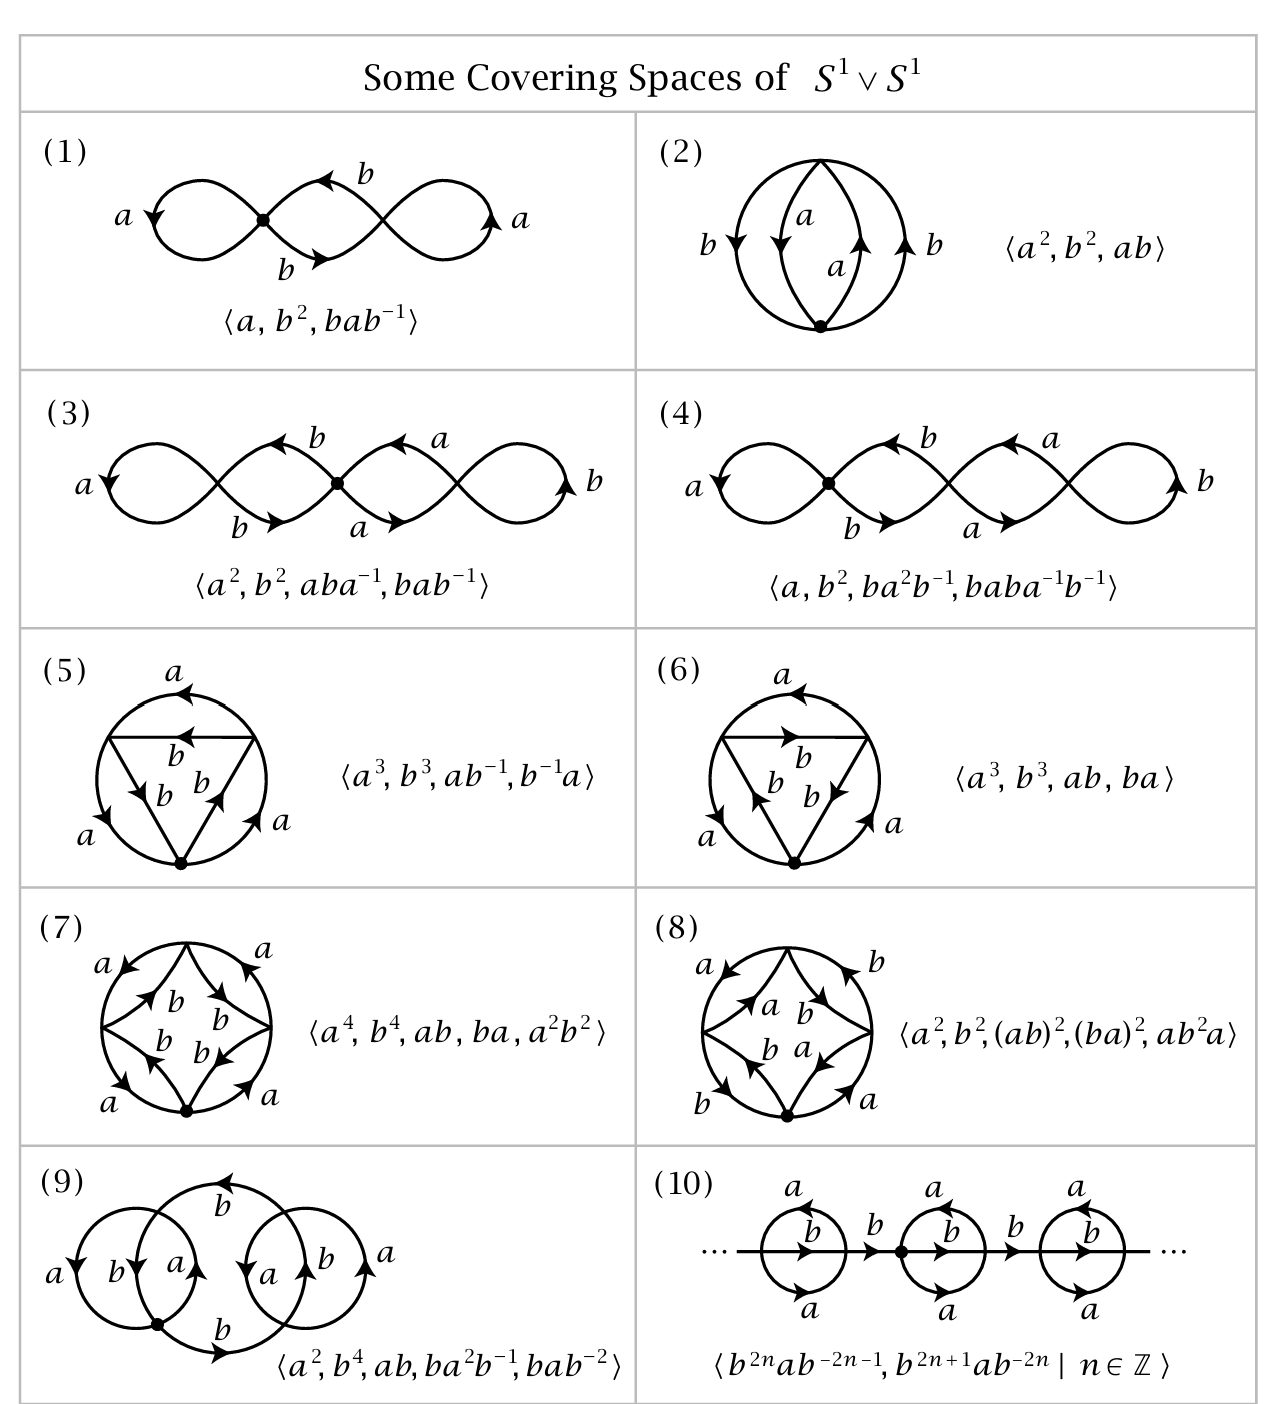
\includegraphics[scale=0.7]{covering space of eight.png}
        \centering
\end{figure}
\begin{coro}
    Free group of free $2$ has free subgroup of rank $3,4,5$ and countable caridinity.
\end{coro}
% \begin{defn}[universal covering space]
%     Suppose $p: E \rightarrow B$ is a covering map, with $p\left(e_0\right)=b_0$. If $E$ is simply connected, then $E$ is called a universal covering space of $B$.
% \end{defn}
\begin{defn}[semi-locally simply connected]
    A space $B$ is said to be semi-locally simply connected 
    if for each $b \in B$, there is a neighborhood $U$ of $b$ such that the homomorphism
    $$
        i_*: \pi_1(U, b) \rightarrow \pi_1(B, b)
    $$
    induced by inclusion is trivial.
\end{defn}
\begin{theo}[existence of covering space]
    Let $B$ be path connected, locally path connected, and semilocally simply connected. Let $b_0 \in B$.
    Given a subgroup $H$ of $\pi_1\left(B, b_0\right)$, there exists a covering map $p: E \rightarrow B$ and a point $e_0 \in p^{-1}\left(b_0\right)$ such that
    $$
        p_*\left(\pi_1\left(E, e_0\right)\right)=H
    $$
\end{theo}
% \begin{theo}
%     Given $p: E \rightarrow B$ with $p\left(e_0\right)=b_0$, let $F$ be the set $F=p^{-1}\left(e_0\right)$. Let
%     $$
%         \Phi: \pi_1\left(B, b_0\right) / H_0 \rightarrow F
%     $$
%     be the lifting correspondence; it is a bijection. Define also a correspondence
%     $$
%         \Psi: \mathcal{C}(E, p, B) \rightarrow F
%     $$
%     by setting $\Psi(h)=h\left(e_0\right)$ for each covering transformation $h: E \rightarrow E$. Since $h$ is uniquely determined once its value at $e_0$ is known, the correspondence $\Psi$ is injective.

%     The image of the map $\Psi$ equals the image under $\Phi$ of the subgroup $N\left(H_0\right) / H_0$ of $\pi_1\left(B, b_0\right) / H_0$ and the bijection
%     $$
%         \Phi^{-1} \circ \Psi: \mathcal{C}(E, p, B) \rightarrow N\left(H_0\right) / H_0
%     $$
%     is an isomorphism of groups.
% \end{theo}








\section{Seifert-van Kampen}
\begin{theo}[Seifert-van Kampen, version 1]
    Suppose $X=U \cup V$, where $U$ and $V$ are open sets of $X$. Suppose that $U \cap V$ is path connected, and that $x_0 \in U \cap V$. Let $i$ and $j$ be the inclusion mappings of $U$ and $V$, respectively, into $X$. Then the images of the induced homomorphisms
    $$
        i_*: \pi_1\left(U, x_0\right) \rightarrow \pi_1\left(X, x_0\right) \quad \text { and } \quad j_*: \pi_1\left(V, x_0\right) \rightarrow \pi_1\left(X, x_0\right)
    $$
    generate $\pi_1\left(X, x_0\right)$.
    \label{theorem:Seifert-van Kampen,version 1}
\end{theo}
\begin{theo}[Seifert-van Kampen, version 2]
    Let $X=U \cup V$, where $U$ and $V$ are open in $X$; assume $U, V$, and $U \cap V$ are path connected; let $x_0 \in U \cap V$. Let $H$ be a group, and let
    $$
        \phi_1: \pi_1\left(U, x_0\right) \longrightarrow H \quad \text { and } \quad \phi_2: \pi_1\left(V, x_0\right) \longrightarrow H
    $$
    be homomorphisms. Let $i_1, i_2, j_1, j_2$ be the homomorphisms indicated in the following diagram, each induced by inclusion.
   % https://q.uiver.app/#q=WzAsNSxbMCwxLCJcXHBpXzEoVVxcY2FwIFYseF8wKSJdLFsxLDAsIlxccGlfMShVLHhfMCkiXSxbMSwyLCJcXHBpXzEoVix4XzApIl0sWzEsMSwiXFxwaV8xKFgseF8wKSJdLFsyLDEsIkgiXSxbMCwxLCJpXzEiXSxbMCwyLCJpXzIiLDJdLFszLDQsIlxcUGhpIiwyXSxbMSw0LCJcXHBoaV8xIl0sWzIsNCwiXFxwaGlfMiJdLFsxLDMsImpfMiJdLFsyLDMsImpfMiIsMl0sWzAsM11d
% https://q.uiver.app/#q=WzAsNSxbMCwxLCJcXHBpXzEoVVxcY2FwIFYseF8wKSJdLFsxLDAsIlxccGlfMShVLHhfMCkiXSxbMSwyLCJcXHBpXzEoVix4XzApIl0sWzEsMSwiXFxwaV8xKFgseF8wKSJdLFsyLDEsIkgiXSxbMCwxLCJpXzEiXSxbMCwyLCJpXzIiLDJdLFszLDQsIlxcUGhpIiwxXSxbMSw0LCJcXHBoaV8xIl0sWzIsNCwiXFxwaGlfMiIsMl0sWzEsMywial8yIl0sWzIsMywial8yIiwyXSxbMCwzXV0=
\[\begin{tikzcd}
	& {\pi_1(U,x_0)} \\
	{\pi_1(U\cap V,x_0)} & {\pi_1(X,x_0)} & H \\
	& {\pi_1(V,x_0)}
	\arrow["{j_2}", from=1-2, to=2-2]
	\arrow["{\phi_1}", from=1-2, to=2-3]
	\arrow["{i_1}", from=2-1, to=1-2]
	\arrow[from=2-1, to=2-2]
	\arrow["{i_2}"', from=2-1, to=3-2]
	\arrow["\Phi"{description}, from=2-2, to=2-3]
	\arrow["{j_2}"', from=3-2, to=2-2]
	\arrow["{\phi_2}"', from=3-2, to=2-3]
\end{tikzcd}\]
    If $\phi_1 \circ i_1=\phi_2 \circ i_2$, then there is a unique homomorphism $\Phi: \pi_1\left(X, x_0\right) \rightarrow H$ such that $\Phi \circ j_1=\phi_1$ and $\Phi \circ j_2=\phi_2$.
    \label{theorem:Seifert-van Kampen,version 2}
\end{theo}
\begin{theo}[Seifert-van Kampen, version 3]
    Assume the hypotheses of the preceding theorem. Let
    $$
        j: \pi_1\left(U, x_0\right) * \pi_1\left(V, x_0\right) \longrightarrow \pi_1\left(X, x_0\right)
    $$
    be the homomorphism of the free product that extends the homomorphisms $j_1$ and $j_2$ induced by inclusion. Then $j$ is surjective, and its kernel is the least normal subgroup $N$ of the free product that contains all elements represented by words of the form
    $$
        \left(i_1(g)^{-1}, i_2(g)\right),
    $$
    for $g \in \pi_1\left(U \cap V, x_0\right)$.
    \label{theorem:Seifert-van Kampen,version 3}
\end{theo}







\newpage
\section{Homotopy equivalence}
\begin{defn}[Homotopy equivalence]
    Let $f: X \rightarrow Y$ and $g: Y \rightarrow X$ be continuous maps. Suppose that the map $g \circ f: X \rightarrow X$ is homotopic to the identity map of $X$, and the map $f \circ g: Y \rightarrow Y$ is homotopic to the identity map of $Y$. Then the maps $f$ and $g$ are called homotopy equivalences, and each is said to be a homotopy inverse of the other.
\end{defn}
\begin{prop}
    $f:X\rightarrow Y $ is a continous map, $\alpha$ is a path from $x_0$ to $x_1$.
    And assume $y_0=f(x_0),y_1=f(x_1)$, we have the following commute diagram
    % https://q.uiver.app/#q=WzAsNCxbMCwwLCJcXHBpKFgseF8wKSJdLFswLDIsIlxccGkoWCx4XzEpIl0sWzIsMCwiXFxwaShZLHlfMCkiXSxbMiwyLCJcXHBpKFkseV8xKSJdLFswLDEsIlxcaGF0e1xcYWxwaGF9Il0sWzAsMiwiZl97Kix4XzB9IiwyXSxbMSwzLCJmX3sqLHhfMX0iXSxbMiwzLCJcXGhhdHtcXGJldGF9IiwyXV0=
    \[\begin{tikzcd}
            {\pi(X,x_0)} && {\pi(Y,y_0)} \\
            \\
            {\pi(X,x_1)} && {\pi(Y,y_1)}
            \arrow["{f_{*,x_0}}"', from=1-1, to=1-3]
            \arrow["{\hat{\alpha}}", from=1-1, to=3-1]
            \arrow["{\hat{\beta}}"', from=1-3, to=3-3]
            \arrow["{f_{*,x_1}}", from=3-1, to=3-3]
        \end{tikzcd}\]
    where $\beta$ is the path $f\circ \alpha$.
    \label{proposition:commute diagram, fundemental group}
\end{prop}
\begin{lem}
    Suppose $\varphi, \psi: X \rightarrow Y$ are continuous, 
    and $H: \varphi \simeq \psi$ is a homotopy. 
    For any $p \in X$, let $h$ be the path in $Y$ from $\varphi(p)$ to $\psi(p)$ 
    defined by $h(t)=H(p, t)$, and let $\Phi_h: \pi_1(Y, \varphi(p)) \rightarrow \pi_1(Y, \psi(p))$ 
    be the isomorphism defined in Proposition\ref{proposition: fundamental group, isomorphism induced by path}. 
    Then the following diagram commutes:% https://q.uiver.app/#q=WzAsMyxbMCwxLCJcXHBpXzEoWCxwKSJdLFsxLDAsIlxccGlfMShYLFxccHNpKFxcdmFycGhpIChwKSkpIl0sWzEsMiwiXFxwaV8xKFgscCkiXSxbMCwxLCIoXFxwc2lcXGNpcmNcXHZhcnBoaSlfKiJdLFswLDIsIlxcdGV4dHtpZH1fKiIsMl0sWzEsMiwiXFxQaGlfaCJdXQ==
    % https://q.uiver.app/#q=WzAsMyxbMCwxLCJcXHBpXzEoWCxwKSJdLFsxLDAsIlxccGlfMShZLFxcdmFycGhpKHApKSJdLFsxLDIsIlxccGlfMShZLFxccHNpKHApKSJdLFswLDEsIlxcdmFycGhpXyoiXSxbMCwyLCJcXHBzaV8qIiwyXSxbMSwyLCJcXFBoaV9oIl1d
\[\begin{tikzcd}
	& {\pi_1(Y,\varphi(p))} \\
	{\pi_1(X,p)} \\
	& {\pi_1(Y,\psi(p))}
	\arrow["{\Phi_h}", from=1-2, to=3-2]
	\arrow["{\varphi_*}", from=2-1, to=1-2]
	\arrow["{\psi_*}"', from=2-1, to=3-2]
\end{tikzcd}\]
\end{lem}

\begin{theo}
    If $\varphi: X \rightarrow Y, \psi:Y\rightarrow X$ 
    is a homotopy equivalence, then for any point $p \in X, \varphi_*: \pi_1(X, p) \rightarrow \pi_1(Y, \varphi(p))$ is an isomorphism.
    \label{theorem: homotopy equivanlece induces fundamental group isomorphism}
\end{theo}
\begin{prooff}
    From above lemma, we have commutative diagram 
    \[\begin{tikzcd}
        & {\pi_1(X,\psi(\varphi (p)))} \\
        {\pi_1(X,p)} \\
        & {\pi_1(X,p)}
        \arrow["{\Phi_h}", from=1-2, to=3-2]
        \arrow["{(\psi\circ\varphi)_*}", from=2-1, to=1-2]
        \arrow["{\text{id}_*}"', from=2-1, to=3-2]
    \end{tikzcd}\]
    Hence, $\varphi_*$ is injective. Similarly, we have the following commutative diagram 
    % https://q.uiver.app/#q=WzAsMyxbMCwxLCJcXHBpXzEoWSxcXHZhcnBoaShwKSkiXSxbMSwwLCJcXHBpXzEoWSxcXHZhcnBoaVxccHNpXFx2YXJwaGkgKHApKSkiXSxbMSwyLCJcXHBpXzEoWSxcXHZhcnBoaShwKSkiXSxbMCwxLCIoXFx2YXJwaGlcXGNpcmNcXHBzaSlfKiJdLFswLDIsIlxcdGV4dHtpZH1fKiIsMl0sWzEsMiwiXFxQaGlfZyJdXQ==
\[\begin{tikzcd}
	& {\pi_1(Y,\varphi\psi\varphi (p)))} \\
	{\pi_1(Y,\varphi(p))} \\
	& {\pi_1(Y,\varphi(p))}
	\arrow["{\Phi_g}", from=1-2, to=3-2]
	\arrow["{(\varphi\circ\psi)_*}", from=2-1, to=1-2]
	\arrow["{\text{id}_*}"', from=2-1, to=3-2]
\end{tikzcd}\]
    From Proposition\ref{proposition:commute diagram, fundemental group}, we have a commutative diagram 
    % https://q.uiver.app/#q=WzAsNCxbMCwxLCJcXHBpXzEoWCxwKSJdLFsxLDEsIlxccGlfMShZLFxcdmFycGhpKHApKSJdLFswLDAsIlxccGlfMShYLFxccHNpXFx2YXJwaGkocCkpIl0sWzEsMCwiXFxwaV8xKFksXFx2YXJwaGlcXHBzaVxcdmFycGhpKHApKSJdLFswLDEsIlxcdmFycGhpXyoiXSxbMCwyXSxbMSwzXSxbMiwzLCJcXHZhcnBoaV97KixcXHBzaVxcdmFycGhpKHApfSJdXQ==
\[\begin{tikzcd}
	{\pi_1(X,\psi\varphi(p))} & {\pi_1(Y,\varphi\psi\varphi(p))} \\
	{\pi_1(X,p)} & {\pi_1(Y,\varphi(p))}
	\arrow["{\varphi_{*,\psi\varphi(p)}}", from=1-1, to=1-2]
	\arrow[from=2-1, to=1-1]
	\arrow["{\varphi_*}", from=2-1, to=2-2]
	\arrow[from=2-2, to=1-2]
\end{tikzcd}\]
Above lemma shows $\varphi_{*,\psi\varphi(p)}$ is surjective, hence $\varphi_*$ is surjective. 




\end{prooff}

% \begin{prop}[correspondence between path-way connected components]
%     There's a one-to-one correspondence between path-way connected components of $X$
%     and path-way connected components of $Y$.
% \end{prop}




\begin{defn}[retraction]
    If $A \subset X$, a retraction of $X$ onto $A$ is a continuous map $r: X \rightarrow A$ such that $r|_A$ is the identity map of $A$. If such a map $r$ exists, we say that $A$ is a retract of $X$.
\end{defn}
\begin{prop}
    If $A$ is a retract of $X$, then the homomorphism of fundamental groups induced by inclusion $j: A \rightarrow X$ is injective.
    \label{proposition:retraction induce injective homomorphism}
\end{prop}
\begin{defn}[deformation retract]
    Let $A$ be a subspace of $X$. We say that $A$ is a deformation retract of $X$
    if the identity map of $X$ is homotopic to
    a map that carries all of $X$ into $A$, such that each point of $A$ remains
    fixed during the homotopy.
\end{defn}
\begin{prooff}
    $A$ is a deformation retract of $X$ if and only if there's $H:X\times I\rightarrow X$
    such that $H(x,0)=x$ for all $x\in X$, $H(a,1)=a$ for all $a\in A$ and $H(x,1)\in A$ for all $x\in X$.
\end{prooff}
\begin{prop}
    $r:X\rightarrow A$ gives a deformation retract from $X$ to $A$ if and only if there's homotopy $H(x,t)$ between $\text{id}_X$ and $i\circ r$.
    We call such $H(x,t)$ also a deformation retract.
\end{prop}
\begin{prop}[deformation retract induces fundamental group isomorphism]
    Let $A$ be a deformation retract of $X$; let $x_0 \in A$. Then the inclusion тар
    $$
        j:\left(A, x_0\right) \rightarrow\left(X, x_0\right)
    $$
    induces an isomorphism of fundamental groups.
\end{prop}
\begin{prooff}
    By Theorem\ref{theorem: homotopy equivanlece induces fundamental group isomorphism}.
\end{prooff}

\begin{defn}[contractible space]
    We call a topological space contractible if it is homotopy equivalent to a one-point space.
\end{defn}
\begin{prop}
    $X$ is contractible if and only if $\text{id}:X\rightarrow X$ is nulhomotopic.
\end{prop}
\begin{exam}
    $X$ is a topological space, cone of $X$ is the space $X\times [0,1]/\sim$, where $\sim$ means the points in $X\times \bbrace{1}$ are all equivalent.
    In general, we denote it by $CX$. Also,
    it's easy to say that $X\times \bbrace{1}$ with subspace topology in $CX$ is isomorphic to $X$.
\end{exam}
\begin{lem}
    $f:X\rightarrow Y$ is a quotient map, $A\subset X$. $r:X\rightarrow A$ is a deformation retract,
    and we denote the homotopy between $i\circ r:X\rightarrow X$,
    and $\text{id}:X\rightarrow X$ by $H(x,t)$.
    If $f(x)=f(y)$ implies $f(H(x,t))=f(H(y,t))$, $f(A)$ is a deformation retract of $Y$.
    \label{lemma:quotient,deformation retract}
\end{lem}
\begin{prooff}
    % https://q.uiver.app/#q=WzAsNCxbMCwwLCJYXFx0aW1lcyBJIl0sWzIsMCwiWCJdLFsyLDIsIlkiXSxbMCwyLCIgWVxcdGltZXMgSSJdLFswLDEsIkgiXSxbMSwyXSxbMywyLCJHIiwyXSxbMCwzLCJmXFx0aW1lcyBcXHRleHR7aWR9IiwyXV0=
    % https://q.uiver.app/#q=WzAsNCxbMCwwLCJYXFx0aW1lcyBJIl0sWzIsMCwiWCJdLFsyLDIsIlkiXSxbMCwyLCIgWVxcdGltZXMgSSJdLFswLDEsIkgiXSxbMSwyLCJmIl0sWzMsMiwiRyIsMix7InN0eWxlIjp7ImJvZHkiOnsibmFtZSI6ImRhc2hlZCJ9fX1dLFswLDMsImZcXHRpbWVzIFxcdGV4dHtpZH0iLDJdXQ==
    \[\begin{tikzcd}
            {X\times I} && X \\
            \\
            { Y\times I} && Y
            \arrow["H", from=1-1, to=1-3]
            \arrow["{f\times \text{id}}"', from=1-1, to=3-1]
            \arrow["f", from=1-3, to=3-3]
            \arrow["G"', dashed, from=3-1, to=3-3]
        \end{tikzcd}\]
    By Proposition~\ref{proposition:quotient map,product}, $f\times \text{id}$ is a quotient map, then by
    Proposition~\ref{proposition:universal proptery of quotient map}, there's a uniquness continous map $G$ makes the diagram commute.
    Then it's easy to check $y\mapsto G(y,1)$ is a deformation retract of $Y$ onto $f(B)$.
\end{prooff}
\begin{prop}
    $CX$ is contractible.
\end{prop}
\begin{prooff}
    Consider
    \begin{align*}
        H:(X\times I)\times I \rightarrow X\times I \\
        (x,t,s)\mapsto (x,(1-s)t+s\cdot 1)
    \end{align*}
    and use Lemma~\ref{lemma:quotient,deformation retract}.
\end{prooff}
\begin{prop}
    Show that a map $f:X\rightarrow Y$ is nullhomotopic if and only if it extends to a map $F:CX\rightarrow Y$.
    \label{proposition:X-Y nulhomotopic iff CX-Y}
\end{prop}
\begin{prooff}
    "only if":
    Consider $H:X\times I\rightarrow Y$ is a homotopy between $f$ and a constant map, then
    by Proposition~\ref{proposition:universal proptery of quotient map}, $H$ induce a continous map $F$ between $CX$ and $Y$
    which makes the following diagram commute
    % https://q.uiver.app/#q=WzAsMyxbMCwwLCJYXFx0aW1lcyBJIl0sWzAsMiwiWFxcdGltZXMgSS9cXHNpbSJdLFsyLDIsIlkiXSxbMCwxLCJcXHBpIl0sWzAsMiwiSCIsMl0sWzEsMiwiXFx0aWxkZXtIfSIsMCx7InN0eWxlIjp7ImJvZHkiOnsibmFtZSI6ImRhc2hlZCJ9fX1dXQ==
    \[\begin{tikzcd}
            {X\times I} \\
            \\
            {X\times I/\sim} && Y
            \arrow["\pi", from=1-1, to=3-1]
            \arrow["H", from=1-1, to=3-3]
            \arrow["F", dashed, from=3-1, to=3-3]
        \end{tikzcd}\]
    "if": Consider the composition $H:X\times I \rarr{\pi} CX \rarr{F} Y$
\end{prooff}


\begin{theo}
    Let $h: \bb{S}^1 \rightarrow X$ be a continuous map. 
    Then the following conditions are equivalent:
    \begin{enumerate}[(1)]
        \item $h$ is nulhomotopic.
        \item $h$ extends to a continuous map $k: B^2 \rightarrow X$.
        \item $(h_{x_0})_*$ is the trivial homomorphism of fundamental groups for all $x_0\in \bb{S}^1$
    \end{enumerate}
\end{theo}
\begin{prooff}
    (1) $\Leftrightarrow$ (2): By Proposition~\ref{proposition:X-Y nulhomotopic iff CX-Y}.

    (1) $\Rightarrow$ (3): By Theorem\ref{theorem: homotopy equivanlece induces fundamental group isomorphism}. 

    (3) $\Rightarrow$ (1): Take $x_0=1$.
    Since $h_*$ is trivial, there's $H:I\times I\rightarrow X$ such that $H(x,0)=h(1), H(x,1)=h(\text{e}^{2\pi \text{i}x})$.
    Let $p_0:I\rightarrow S^1 \quad x\mapsto \text{e}^{2\pi \text{i}x}$, then $p_0\times \text{id}:I\times I\rightarrow S^1 \times I$ is a quotient map,
    hence by Proposition~\ref{proposition:universal proptery of quotient map}, there's $\tilde{H}$ making the following diagram commute
    % https://q.uiver.app/#q=WzAsMyxbMCwwLCJJXFx0aW1lcyBJIl0sWzAsMiwiU14xXFx0aW1lcyBJIl0sWzIsMiwiWCJdLFswLDEsInBfMFxcdGltZXMgXFx0ZXh0e2lkfSJdLFsxLDIsIlxcdGlsZGV7SH0iLDAseyJzdHlsZSI6eyJib2R5Ijp7Im5hbWUiOiJkYXNoZWQifX19XSxbMCwyLCJIIiwyXV0=
    \[\begin{tikzcd}
            {I\times I} \\
            \\
            {S^1\times I} && X
            \arrow["{p_0\times \text{id}}", from=1-1, to=3-1]
            \arrow["H"', from=1-1, to=3-3]
            \arrow["{\tilde{H}}", dashed, from=3-1, to=3-3]
        \end{tikzcd}\]
    and $\tilde{H}$ is what we need.
\end{prooff}
\begin{coro}
    Identity map $\bb{S}^1\rightarrow \bb{S}^1$ are not nulhomotopic.
\end{coro}
\begin{theo}
    Given a continuous map $v:\bb{S}^1\rightarrow \bb{R}^2-\bbrace{0}$, there exists a point of $S^1$ where the vector field points directly inward and a point of $S^1$ where it points directly outward.
\end{theo}
% \begin{prooff}
%     Let $w$ be its restriction to $S^1$. Because the map $w$ extends to a map of $B^2$ into $\mathbb{R}^2-0$, it is nulhomotopic.

%     On the other hand, $w$ is homotopic to the inclusion map $j: S^1 \rightarrow \mathbb{R}^2-0$. Figure 55.3 illustrates the homotopy; one defines it formally by the equation
%     $$
%         F(x, t)=t x+(1-t) w(x),
%     $$
%     for $x \in S^1$. We must show that $F(x, t) \neq 0$. Clearly, $F(x, t) \neq 0$ for $t=0$ and $t=1$. If $F(x, t)=0$ for some $t$ with $0<t<1$, then $t x+(1-t) w(x)=0$, so that $w(x)$ equals a negative scalar multiple of $x$. But this means that $w(x)$ points directly inward at $x$ ! Hence $F$ maps $S^1 \times I$ into $\mathbb{R}^2-0$, as desired.
%     It follows that $j$ is nulhomotopic, contradicting the preceding corollary.
%     To show that $v$ points directly outward at some point of $S^1$, we apply the result just proved to the vector field $(x,-v(x))$.
% \end{prooff}
\begin{theo}[Brouwer fixed-point theorem for the disc]
    If $f: B^2 \rightarrow B^2$ is continuous, then there exists a point $x \in B^2$ such that $f(x)=x$.
\end{theo}
% \begin{prooff}
%     We proceed by contradiction. Suppose that $f(x) \neq x$ for every $x$ in $B^2$. Then defining $v(x)=f(x)-x$ gives us a nonvanishing vector field $(x, v(x))$ on $B^2$. But the vector field $v$ cannot point directly outward at any point $x$ of $S^1$, for that would mean
%     $$
%         f(x)-x=a x
%     $$
%     for some positive real number $a$, so that $f(x)=(1+a) x$ would lie outside the unit ball $B^2$. We thus arrive at a contradiction.
% \end{prooff}
\begin{exam}[Fundamental theorem of Algebra]
    A polynomial equation
    $$
        x^n+a_{n-1} x^{n-1}+\cdots+a_1 x+a_0=0
    $$
    of degree $n>0$ with complex coefficients has at least one complex root.
\end{exam}
\begin{prooff}
    Step 1 : Let $f:\bb{S}^1\rightarrow \bb{S}^1: z\mapsto z^n$. Then by Theorem~\ref{tehorem:lifting correspondence}, the induced group homomorphism $f_*:\pi(\bb{S}^1,1)\rightarrow \pi(\bb{S}^1,1)$ is injective.

    Step 2 : We show that if $g: \bb{S}^1 \rightarrow \mathbb{R}^2-0$ is the map $g(z)=z^n$, then $g$ is not nulhomotopic.

    Let $j:\bb{S}^1\rightarrow \mathbb{R}^2-0$ be inclusion. Notice that $j\circ f=g $, then by Theorem~\ref{proposition:retraction induce injective homomorphism}, $g_*$ is injective. Hence $g$ is not nulhomotopic.

    Step 3 : Now we prove a stronger case of the theorem. Given a polynomial equation
    $$
        x^n+a_{n-1} x^{n-1}+\cdots+a_1 x+a_0=0,
    $$
    we assume that
    $$
        \left|a_{n-1}\right|+\cdots+\left|a_1\right|+\left|a_0\right|<1
    $$
    and show that the equation has a root lying in the unit ball $B^2$. Notice that if we replace $x$ by $cx$ for a sufficiently large $c>0$, we can obtain the original Fundemental Theorem of Algebra.
    Assume it has no such root. Then we can define a map $k: B^2 \rightarrow \mathbb{R}^2-0$ by the equation
    $$
        k(z)=z^n+a_{n-1} z^{n-1}+\cdots+a_1 z+a_0 .
    $$
    Let $h$ be the restriction of $k$ to $S^1$. Because $h$ extends to a map of the unit ball into $\mathbb{R}^2-0$, the map $h$ is nulhomotopic.

    On the other hand, we shall define a homotopy $F$ between $h$ and the map $g$ of Step 2; since $g$ is not nulhomotopic, we have a contradiction. We define $F: S^1 \times I \rightarrow$ $\mathbb{R}^2-0$ by the equation
    $$
        F(z, t)=z^n+t\left(a_{n-1} z^{n-1}+\cdots+a_0\right) .
    $$

    $F(z, t)$ never equals $0$ because
    $$
        \begin{aligned}
            |F(z, t)| & \geq\left|z^n\right|-\left|t\left(a_{n-1} z^{n-1}+\cdots+a_0\right)\right| \\
                      & \geq 1-t\left(\left|a_{n-1} z^{n-1}\right|+\cdots+\left|a_0\right|\right)  \\
                      & =1-t\left(\left|a_{n-1}\right|+\cdots+\left|a_0\right|\right)>0 .
        \end{aligned}
    $$
\end{prooff}

\begin{exam}
    \begin{align*}
        r: \bb{R}^n-\bbrace{0}\rightarrow \bb{S}^{n-1} \\
        x\mapsto \frac{x}{||x||}
    \end{align*}
    gives us a deformation retract of $\bb{R}^n-\bbrace{0}$ onto $\bb{S}^{n-1}$.
\end{exam}

\begin{prop}
    $f,g\in C(X,S^n)$, if $f$ and $g$ satisfies $f(x)\neq -g(x),\forall x\in X$, then $f\simeq g$.
\end{prop}
\begin{prooff}
    Consider
    \begin{equation*}
        H(x,t)=\frac{(1-t)f(x)+tg(x)}{||(1-t)f(x)+tg(x)||}
    \end{equation*}
\end{prooff}
\begin{prop}
    $f,g\in C(X,E)$, $E$ is a convex subgroup of $\bb{R}^n$, then $f\simeq g$.
    by the homotopic map $H(x,t)=(1-t)f(x)+tg(x)$.
\end{prop}
% \begin{theo}
%     Let $h, k: X \rightarrow Y$ be continuous maps; let $h\left(x_0\right)=y_0$ and $k\left(x_0\right)=y_1$. If $h$ and $k$ are homotopic, there is a path $\alpha$ in $Y$ from $y_0$ to $y_1$ such that $k_*=\hat{\alpha} \circ h_*$. Indeed, if $H: X \times I \rightarrow Y$ is the homotopy between $h$ and $k$, then $\alpha$ is the path $\alpha(t)=H\left(x_0, t\right)$.
%     % https://q.uiver.app/#q=WzAsMyxbMCwwLCJcXHBpXzEoWCx4XzApIl0sWzIsMCwiXFxwaV8xKFkseV8wKSJdLFsyLDIsIlxccGlfMShZLHlfMSkiXSxbMCwxLCJoXyoiXSxbMSwyLCJcXGhhdHtcXGFscGhhfSJdLFswLDIsImtfKiIsMl1d
%     \[\begin{tikzcd}
%             {\pi_1(X,x_0)} && {\pi_1(Y,y_0)} \\
%             \\
%             && {\pi_1(Y,y_1)}
%             \arrow["{h_*}", from=1-1, to=1-3]
%             \arrow["{\hat{\alpha}}", from=1-3, to=3-3]
%             \arrow["{k_*}"', from=1-1, to=3-3]
%         \end{tikzcd}\]
% \end{theo}
% \begin{prooff}
%     Let $f: I \rightarrow X$ be a loop in $X$ based at $x_0$. We must show that
%     $$
%         k_*([f])=\hat{\alpha}\left(h_*([f]) .\right.
%     $$

%     This equation states that $[k \circ f]=[\bar{\alpha}] *[h \circ f] *[\alpha]$, or equivalently, that
%     $$
%         [\alpha] *[k \circ f]=[h \circ f] *[\alpha] .
%     $$

%     This is the equation we shall verify.
%     To begin, consider the loops $f_0$ and $f_1$ in the space $X \times I$ given by the equations
%     $$
%         f_0(s)=(f(s), 0) \quad \text { and } \quad f_1(s)=(f(s), 1) .
%     $$

%     Consider also the path $c$ in $X \times I$ given by the equation
%     $$
%         c(t)=\left(x_0, t\right) .
%     $$
%     Then $H \circ f_0=h \circ f$ and $H \circ f_1=k \circ f$, while $H \circ c$ equals the path $\alpha$.
%     Let $F: I \times I \rightarrow X \times I$ be the map $F(s, t)=(f(s), t)$. Consider the following paths in $I \times I$, which run along the four edges of $I \times I$ :
%     $$
%         \begin{array}{lll}
%             \beta_0(s)=(s, 0)  & \text { and } & \beta_1(s)=(s, 1),   \\
%             \gamma_0(t)=(0, t) & \text { and } & \gamma_1(t)=(1, t) .
%         \end{array}
%     $$

%     Then $F \circ \beta_0=f_0$ and $F \circ \beta_1=f_1$, while $F \circ \gamma_0=F \circ \gamma_1=c$.
%     The broken-line paths $\beta_0 * \gamma_1$ and $\gamma_0 * \beta_1$ are paths in $I \times I$ from $(0,0)$ to $(1,1)$; since $I \times I$ is convex, there is a path homotopy $G$ between them. Then $F \circ G$ is a path homotopy in $X \times I$ between $f_0 * c$ and $c * f_1$. And $H \circ(F \circ G)$ is a path homotopy in $Y$ between
%     $$
%         \begin{aligned}
%              & \left(H \circ f_0\right) *(H \circ c)=(h \circ f) * \alpha \quad \text { and } \\
%              & (H \circ c) *\left(H \circ f_1\right)=\alpha *(k \circ f),
%         \end{aligned}
%     $$
% \end{prooff}
% \begin{coro}
%     Let $h, k: X \rightarrow Y$ be homotopic continuous maps; let $h\left(x_0\right)=y_0$ and $k\left(x_0\right)=y_1$. If $h_*$ is injective, or surjective, or trivial, so is $k_*$.
% \end{coro}
% \begin{coro}
%     Let $h: X \rightarrow Y$. If $h$ is nulhomotopic, then $h_*$ is the trivial homomorphism.
% \end{coro}
% \begin{coro}
%     Let $f: X \rightarrow Y$ be continuous; let $f\left(x_0\right)=y_0$. If $f$ is a homotopy equivalence, then
%     $$
%         f_*: \pi_1\left(X, x_0\right) \longrightarrow \pi_1\left(Y, y_0\right)
%     $$
%     is an isomorphism.
% \end{coro}
% \begin{prooff}
%     Let $g: Y \rightarrow X$ be a homotopy inverse for $f$. Consider the maps
%     $$
%         \left(X, x_0\right) \xrightarrow{f}\left(Y, y_0\right) \xrightarrow{g}\left(X, x_1\right) \xrightarrow{f}\left(Y, y_1\right),
%     $$
%     where $x_1=g\left(y_0\right)$ and $y_1=f\left(x_1\right)$. We have the corresponding induced homomorphisms:

%     $$
%         \pi_1\left(X, x_0\right) \xrightarrow{\left(f_{x_0}\right)_*} \pi_1\left(Y, y_0\right)\xrightarrow{g_*}  \pi_1\left(X, x_1\right) \xrightarrow{\left(f_{x_1}\right)_*} \pi_1\left(Y, y_1\right)
%     $$

%     Now
%     $$
%         g \circ f:\left(X, x_0\right) \longrightarrow\left(X, x_1\right)
%     $$
%     is by hypothesis homotopic to the identity map, so there is a path $\alpha$ in $X$ such that
%     $$
%         (g \circ f)_*=\hat{\alpha} \circ\left(i_X\right)_*=\hat{\alpha} .
%     $$

%     It follows that $(g \circ f)_*=g_* \circ\left(f_{x_0}\right)_*$ is an isomorphism. Hence $g_*$ is surjective.
%     Similarly, because $f \circ g$ is homotopic to the identity map $i_Y$, the homomorphism $(f \circ g)_*=\left(f_{x_1}\right)_* \circ g_*=\hat{\beta}$ for some path $\beta$ in Y. Hence $g_*$ is injective.

% \end{prooff}



\begin{coro}
    For $n\ge 2$, $\bb{S}^n$ is simply connected.
    \label{corollary:Sn is simply connect}
\end{coro}
\begin{prooff}
    Let $p=(0, \ldots, 0,1) \in \mathbb{R}^{n+1}$ and $q=(0, \ldots, 0,-1)$ be the "north pole" and the "south pole" of $S^n$, respectively.

    Step 1. We show that if $n \geq 1$, the punctured sphere $S^n-p$ is homeomorphic to $\mathbb{R}^n$.
    Define $f:\left(S^n-p\right) \rightarrow \mathbb{R}^n$ by the equation
    $$
        f(x)=f\left(x_1, \ldots, x_{n+1}\right)=\frac{1}{1-x_{n+1}}\left(x_1, \ldots, x_n\right) .
    $$

    One checks that $f$ is a homeomorphism by showing that the map $g: \mathbb{R}^n \rightarrow\left(S^n-p\right)$ given by
    $$
        g(y)=g\left(y_1, \ldots, y_n\right)=\left(t(y) \cdot y_1, \ldots, t(y) \cdot y_n, 1-t(y)\right),
    $$
    where $t(y)=2 /\left(1+\|y\|^2\right)$, is a right and left inverse for $f$.
    Note that the reflection map $\left(x_1, \ldots, x_{n+1}\right) \rightarrow\left(x_1, \ldots, x_n,-x_{n+1}\right)$ defines a homeomorphism of $S^n-p$ with $S^n-q$, so the latter is also homeomorphic to $\mathbb{R}^n$.

    Step 2. We prove the theorem. Let $U$ and $V$ be the open sets $U=S^n-p$ and $V=S^n-q$ of $S^n$.

    Note first that for $n \geq 1$, the sphere $S^n$ is path connected. This follows from the fact that $U$ and $V$ are path connected (being homeomorphic to $\mathbb{R}^n$ ) and have the point $(1,0, \ldots, 0)$ of $S^n$ in common.

    Now we show that for $n \geq 2$, the sphere $S^n$ is simply connected. The spaces $U$ and $V$ are simply connected, being homeomorphic to $\mathbb{R}^n$. 
    Their intersection equals $S^n-p-q$, which is homeomorphic under stereographic projection to $\mathbb{R}^n-0$. 
    The latter space is path connected, for every point of $\mathbb{R}^n-0$ can be joined to a point of $S^{n-1}$ by a straight-line path, and $S^{n-1}$ is path connected if $n \geq 2$.
    Then by Theorem~\ref{theorem:Seifert-van Kampen,version 1}, we finish the proof.
\end{prooff}
\begin{prop}
    $\pi_1\left(X \times Y, x_0 \times y_0\right)$ is isomorphic with $\pi_1\left(X, x_0\right) \times \pi_1\left(Y, y_0\right)$. In particular,
    let $p: X \times Y \rightarrow X$ and $q: X \times Y \rightarrow Y$ be the projection mappings. If we use the base points indicated in the statement of the theorem, we have induced homomorphisms
    $$
        \begin{aligned}
             & p_*: \pi_1\left(X \times Y, x_0 \times y_0\right) \longrightarrow \pi_1\left(X, x_0\right),  \\
             & q_*: \pi_1\left(X \times Y, x_0 \times y_0\right) \longrightarrow \pi_1\left(Y, y_0\right) .
        \end{aligned}
    $$

    We define a homomorphism
    $$
        \Phi: \pi_1\left(X \times Y, x_0 \times y_0\right) \longrightarrow \pi_1\left(X, x_0\right) \times \pi_1\left(Y, y_0\right)
    $$
    by the equation
    $$
        \Phi([f])=p_*([f]) \times q_*([f])=[p \circ f] \times[q \circ f] .
    $$
    then $\Phi$ is an isomorphism.
\end{prop}
\begin{prop}
    $\bb{R}\bb{P}^n\simeq \bb{S}^n/\bbrace{x\sim -x}\simeq \bb{D}^n/\bb{S}^{n-1}$
    where the second isomorphism is given by
    \begin{align*}
        (z_1,\dots,z_n) \in \bb{D}^n/\bb{S}^{n-1}\mapsto [z_1,\dots,z_n,\sqrt{1-z_1^2-\dots-z_n^2} \quad  ]\in \bb{R}\bb{P}^n
    \end{align*}
\end{prop}
\begin{exam}
    $\pi(\bb{R}\bb{P}^n,y)\simeq \bb{Z}/2\bb{Z}$
\end{exam}
\begin{prooff}
    Step 1: $p:\bb{S}^n\rightarrow \bb{R}\bb{P}^n \quad (x_0,\dots,x_n)\mapsto [x_0,\dots,x_n]$ is a surjective continuous open map.

    Step 2: $p$ is a covering map.

    It follows from the fact the $\bb{R}\bb{P}^n\simeq \bb{S}^n/\sim $, where $\simeq$ is the equivalence relation defined by $x\sim y$ iff $x=\pm y$.

    Step 3: $\pi(\bb{R}\bb{P}^n,y)\simeq \bb{Z}/2\bb{Z}$

    By Corollary~\ref{corollary:Sn is simply connect} and Theorem~\ref{tehorem:lifting correspondence}.
\end{prooff}





\section{Classifiction of Compact Surface }
\begin{defn}[polygonal representation of topological space]
    % Given a point $c$ of $\mathbb{R}^2$, and given $a>0$, consider the circle of radius $a$ in $\mathbb{R}^2$ with center at $c$. Given a finite sequence $\theta_0<\theta_1<\cdots<\theta_n$ of real numbers, where $n \geq 3$ and $\theta_n=\theta_0+2 \pi$, consider the points $p_i=c+a\left(\cos \theta_i, \sin \theta_i\right)$, which lie on this circle. They are numbered in counterclockwise order around the circle, and $p_n=p_0$. The line through $p_{i-1}$ and $p_i$ splits the plane into two closed half-planes; let $H_i$ be the one that contains all the points $p_k$. Then the space
    % $$
    %     P=H_1 \cap \cdots \cap H_n
    % $$
    % is called the polygonal region determined by the points $p_i$. The points $p_i$ are called the vertices of $P$; the line segment joining $p_{i-1}$ and $p_i$ is called an edge of $P$; the union of the edges of $P$ is denoted $\mathrm{Bd} P$; and $P-\operatorname{Bd} P$ is denoted Int $P$. It is not hard to show that if $p$ is any point of Int $P$, then $P$ is the union of all line segments joining $p$ and points of $\mathrm{Bd} P$, and that two such line segments intersect only in the point $p$.

    % Given a line segment $L$ in $\mathbb{R}^2$, an orientation of $L$ is simply an ordering of its end points; the first, say $a$, is called the initial point, and the second, say $b$, is called the final point, of the oriented line segment. We often say that $L$ is oriented from $\boldsymbol{a}$ to $\boldsymbol{b}$; and we picture the orientation by drawing an arrow on $L$ that points from $a$ towards $b$. If $L^{\prime}$ is another line segment, oriented from $c$ to $d$, then the positive linear map of $L$ onto $L^{\prime}$ is the homeomorphism $h$ that carries the point $x=(1-s) a+s b$ of $L$ to the point $h(x)=(1-s) c+s d$ of $L^{\prime}$.

    % Let $P$ be a polygonal region in the plane. A labelling of the edges of $P$ is a map from the set of edges of $P$ to a set $S$ called the set of labels. Given an orientation of each edge of $P$, and given a labelling of the edges of $P$,
    % we define an equivalence relation on the points of $P$ as follows:
    % Each point of $P$ is equivalent only to itself.
    % Given any two edges of $P$ that have the same label,
    % let $h$ be the positive linear map of one onto the other,
    % and define each point $x$ of the first edge to be equivalent to
    % the point $h(x)$ of the second edge. This relation generates an equivalence relation on $P$.
    % The quotient space $X$ obtained from this equivalence relation is said to have been obtained by pasting the edges of $P$ together according to the given orientations and labelling.

    % Given a finite number $P_1, \ldots, P_k$ of disjoint polygonal regions, along with orientations and a labelling of their edges, one can form a quotient space $X$ in exactly the same way as for a single region, by pasting the edges of these regions together.
    % Also, one specifies orientations and a labelling in a similar way, by means of $k$ labelling schemes.
    % Depending on the particular schemes, the space $X$ one obtains may or may not be connected.
\end{defn}
\begin{lem}
    Let $X$ be a Hausdorff space; let $A$ be a closed path-connected subspace of $X$.
    Suppose that there is a continuous map $h: B^2 \rightarrow X$ that maps $B^2-\bb{S}^1$ bijectively onto $X-A$ and maps $\bb{S}^1$ into $A$. Let $p \in S^1$ and let $a=h(p)$; let $k:\left(S^1, p\right) \rightarrow(A, a)$ be the map obtained by restricting $h$. Then the homomorphism
    $$
        i_*: \pi_1(A, a) \longrightarrow \pi_1(X, a)
    $$
    induced by inclusion is surjective, and its kernel is the least normal subgroup of $\pi_1(A, a)$ containing the image of $k_*: \pi_1\left(S^1, p\right) \rightarrow \pi_1(A, a)$.
    \label{theorem:torus}
\end{lem}
\begin{prop}
    Let $X$ be the wedge of the circles $S_1, \ldots, S_n$; let $p$ be the common point of these circles. Then $\pi_1(X, p)$ is a free group. If $f_i$ is a loop in $S_i$ that represents a generator of $\pi_1\left(S_i, p\right)$, then the loops $f_1, \ldots, f_n$ represent a system of free generators for $\pi_1(X, p)$.
\end{prop}
\begin{prooff}
    By Theorem~\ref{theorem:Seifert-van Kampen,version 3}
\end{prooff}

\begin{coro}
    Let $P$ be a polygonal region; let
    $$
        w=\left(a_{i_1}\right)^{\epsilon_1} \cdots\left(a_{i_n}\right)^{\epsilon_n}
    $$
    be a labelling scheme for the edges of $P$. Let $X$ be the resulting quotient space; let $\pi: P \rightarrow X$ be the quotient map.
    \blue{If $\pi$ maps all the vertices of $P$ to a single point $x_0$ of $X$}, and if $a_1, \ldots, a_k$ are the distinct labels that appear in the labelling scheme, then $\pi_1\left(X, x_0\right)$ is isomorphic to the quotient of the free group on $k$ generators $\alpha_1, \ldots, \alpha_k$ by the least normal subgroup containing the element
    $$
        \left(\alpha_{i_1}\right)^{\epsilon_1} \cdots\left(\alpha_{i_n}\right)^{\epsilon_n} .
    $$
\end{coro}
\begin{defn}
    Let $X$ be a Hausdorff space that is the union of the subspaces $S_1, \ldots, S_n$, each of which is homeomorphic to the unit circle $S^1$. Assume that there is a point $p$ of $X$ such that $S_i \cap S_j=\{p\}$ whenever $i \neq j$. Then $X$ is called the wedge of the circles $S_1, \ldots, S_n$.
\end{defn}
\begin{defn}[dunce cap]
    Let $n$ be a positive integer with $n>1$.
    Let $r: S^1 \rightarrow S^1$ be rotation through the angle $2 \pi / n$,
    mapping the point $(\cos \theta, \sin \theta)$ to the point $(\cos (\theta+$ $2 \pi / n), \sin (\theta+2 \pi / n)$ ).
    Form a quotient space $X$ from the unit ball $B^2$ by identifying each point $x$ of $S^1$ with the points $r(x), r^2(x), \ldots, r^{n-1}(x)$.
    We call it the $n$-fold dunce cap.
\end{defn}
\begin{prooff}
    By Theorem~\ref{theorem:torus}.
\end{prooff}
\begin{figure}[H]
    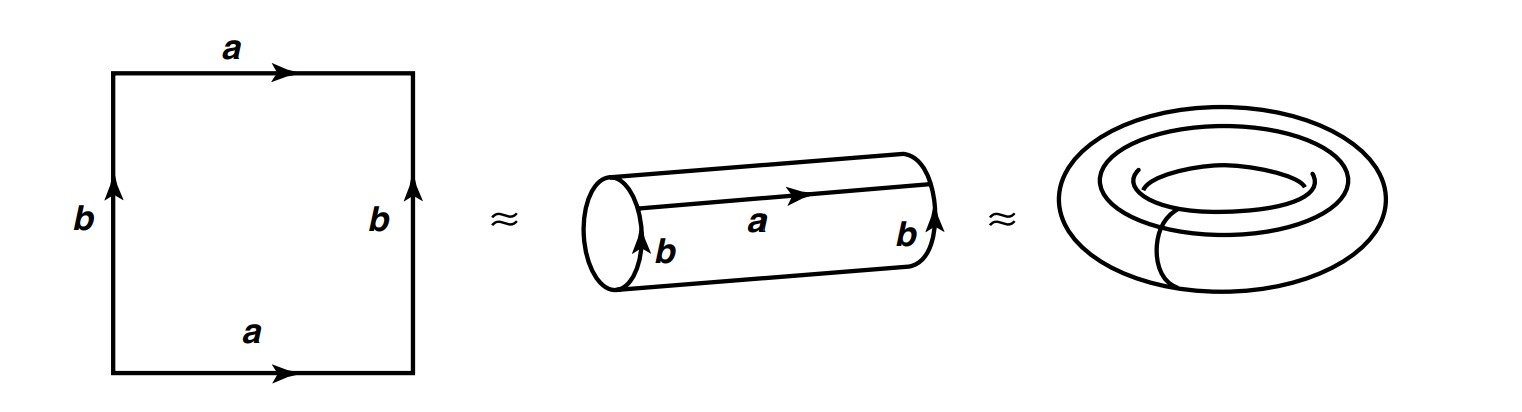
\includegraphics[scale=0.7]{torus2.png}
    \caption{torus}
    \centering
\end{figure}
\begin{figure}[H]
    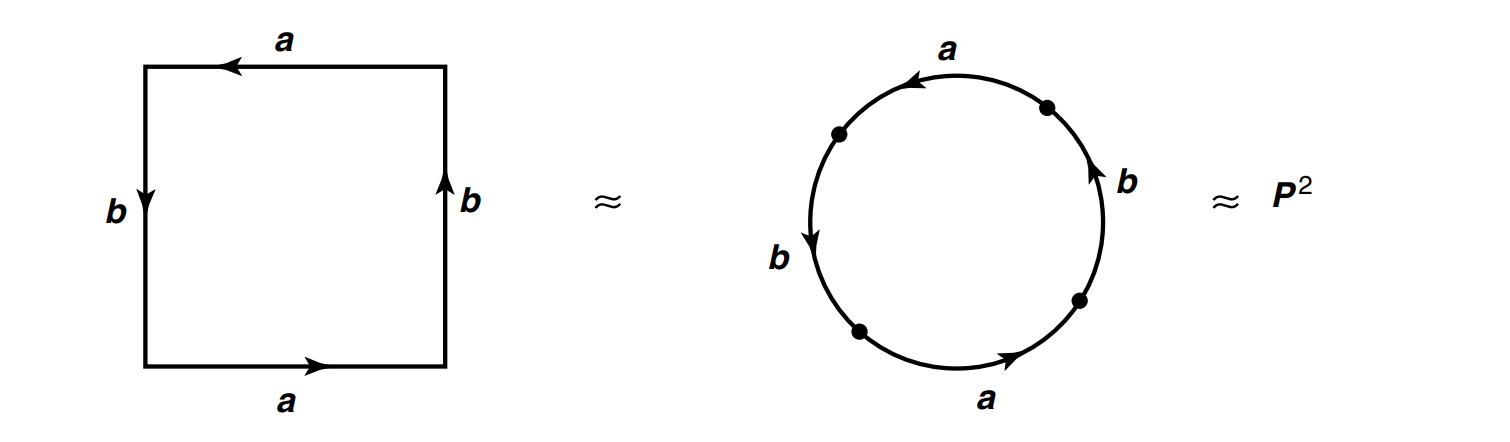
\includegraphics[scale=0.7]{proj1.png}
    \centering
    \caption{projective space}
\end{figure}
\begin{figure}[H]
    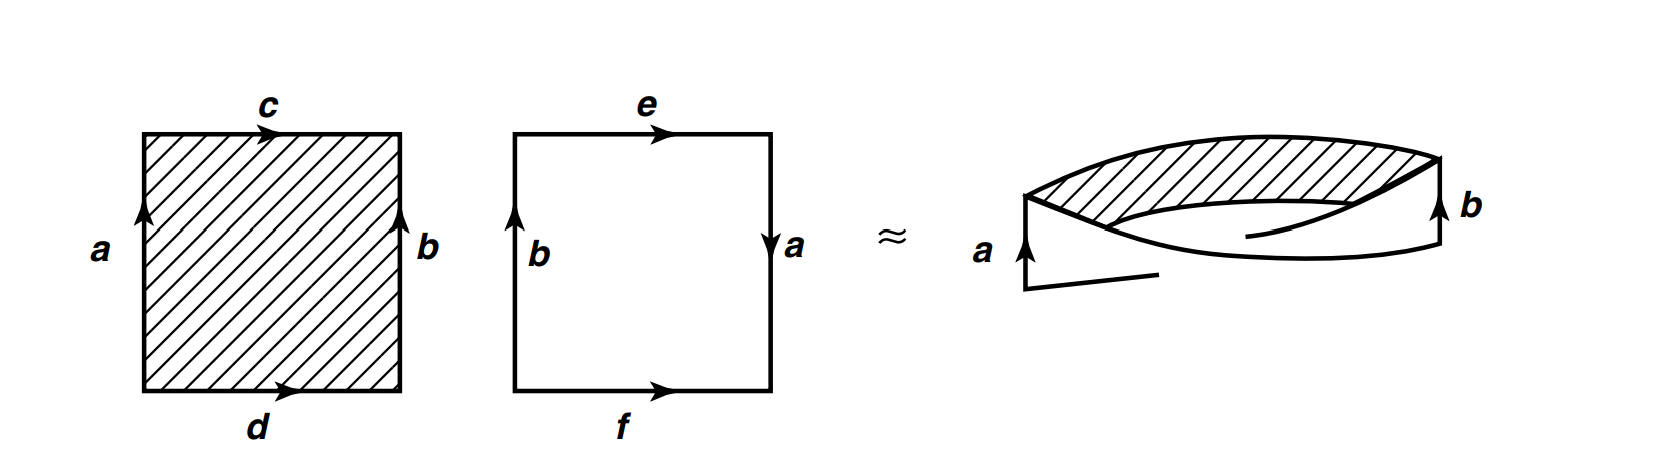
\includegraphics[scale=0.7]{mobi1.png}
    \centering
    \caption{Mobious band}
\end{figure}
\begin{prop}
    Let $X$ be the space obtained from a finite collection of polygonal regions by pasting edges together according to some labelling scheme. Then $X$ is a compact Hausdorff space.
\end{prop}
\begin{theo}
    Consider the space obtained from a $4 n$-sided polygonal region $P$ by means of the labelling scheme
    $$
        \left(a_1 b_1 a_1^{-1} b_1^{-1}\right)\left(a_2 b_2 a_2^{-1} b_2^{-1}\right) \cdots\left(a_n b_n a_n^{-1} b_n^{-1}\right) .
    $$

    This space is called the $n$-fold connected sum of tori, or simply the $n$-fold torus, and denoted $T \# \ldots \# T$.
\end{theo}
\begin{theo}
    Let $X$ denote the $n$-fold torus. Then $\pi_1\left(X, x_0\right)$ is isomorphic to the quotient of the free group on the $2 n$ generators $\alpha_1, \beta_1, \ldots, \alpha_n, \beta_n$ by the least normal subgroup containing the element
    $$
        \left[\alpha_1, \beta_1\right]\left[\alpha_2, \beta_2\right] \cdots\left[\alpha_n, \beta_n\right]
    $$
    where $[\alpha, \beta]=\alpha \beta \alpha^{-1} \beta^{-1}$, as usual.
\end{theo}
\begin{theo}
    Let $m>1$. Consider the space obtained from a $2 m$-sided polygonal region $P$ in the plane by means of the labelling scheme
    $$
        \left(a_1 a_1\right)\left(a_2 a_2\right) \cdots\left(a_m a_m\right)
    $$

    This space is called the $m$-fold connected sum of projective planes, or simply the $\boldsymbol{m}$-fold projective plane, and denoted $P^2 \# \ldots \# P^2$.
\end{theo}
\begin{theo}
    Let $X$ denote the $m$-fold projective plane. Then $\pi_1\left(X, x_0\right)$ is isomorphic to the quotient of the free group on $m$ generators $\alpha_1, \ldots, \alpha_m$ by the least normal subgroup containing the element
    $$
        \left(\alpha_1\right)^2\left(\alpha_2\right)^2 \cdots\left(\alpha_m\right)^2 .
    $$
\end{theo}
\begin{defn}[elementary operations on schemes]
    We now list a number of elementary operations that can be performed on a labelling scheme $w_1, \ldots, w_m$ without affecting the resulting quotient space $X$.
    \begin{enu}
        \item Cut. One can replace the scheme $w_1=y_0 y_1$ by the scheme $y_0 c^{-1}$ and $c y_1$, provided $c$ does not appear elsewhere in the total scheme and $y_0$ and $y_1$ have length at least two.
        \item Paste. One can replace the scheme $y_0 c^{-1}$ and $c y_1$ by the scheme $y_0 y_1$, provided $c$ does not appear elsewhere in the total scheme.
        \item Relabel. One can replace all occurrences of any given label by some other label that does not appear elsewhere in the scheme. Similarly, one can change the sign of the exponent of all occurrences of a given label $a$; this amounts to reversing the orientations of all the edges labelled " $a$ ". Neither of these alterations affects the pasting map.
        \item Permute. One can replace any one of the schemes $w_i$ by a cyclic permutation of $w_i$. Specifically, if $w_i=y_0 y_1$, we can replace $w_i$ by $y_1 y_0$. This amount to renumbering the vertices of the polygonal region $P_i$ so as to begin with a different vertex; it does not affect the resulting quotient space.
        \item Flip. One can replace the scheme
        $$
            w_i=\left(a_{i_1}\right)^{\epsilon_1} \cdots\left(a_{i_n}\right)^{\epsilon_n}
        $$
        by its formal inverse
        $$
            w_i^{-1}=\left(a_{i_n}\right)^{-\epsilon_n} \cdots\left(a_{i_1}\right)^{-\epsilon_1} .
        $$
        This amounts simply to "flipping the polygonal region $P_i$ over.". The order of the vertices is reversed, and so is the orientation of each edge. The quotient space $X$ is not affected.
        \item Cancel. One can replace the scheme $w_i=y_0 a a^{-1} y_1$ by the scheme $y_0 y_1$, provided $a$ does not appear elsewhere in the total scheme and both $y_0$ and $y_1$ have length at least two.
        \begin{figure}[H]
            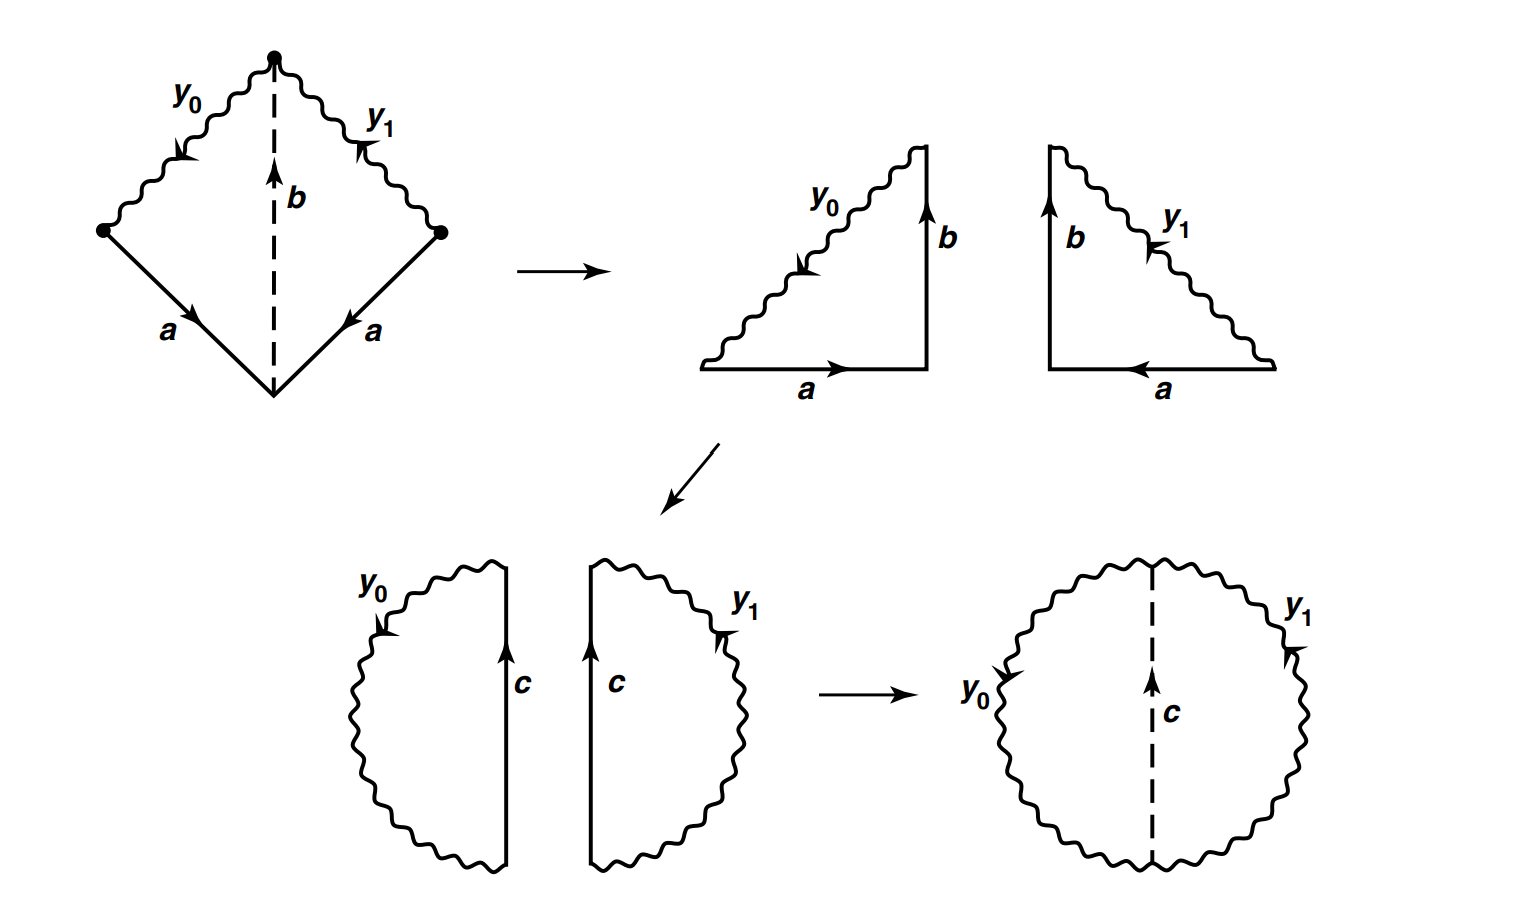
\includegraphics[scale=0.5]{cancel.png}
            \centering
        \end{figure}
    \end{enu}
\end{defn}
\begin{exam}
    The Klein bottle $K$ is the space obtained from the labelling scheme $a b a^{-1} b$ is isomorphic to the 2-fold projective plane $P^2\# P^2(aabb)$ through
    the following elementary operations:
    $$
        \begin{aligned}
            a b a^{-1} b & \longrightarrow a b c^{-1} \text { and } c a^{-1} b\quad \text{by cutting}                                           \\
                         & \longrightarrow c^{-1} a b \text { and } b^{-1} a c^{-1} \quad \text{by permuting the first and flipping the second} \\
                         & \longrightarrow c^{-1} a a c^{-1}\quad \text{ by pasting}                                                            \\
                         & \longrightarrow aacc
        \end{aligned}
    $$
\end{exam}
\begin{theo}
    Suppose $w_1, \ldots, w_k$ is a labelling scheme for the polygonal regions $P_1, \ldots, P_k$. If each label appears exactly twice in this scheme, we call it a proper labelling scheme. Note the important fact:
    If one applies any elementary operation to a proper scheme, one obtains another proper scheme.
\end{theo}
\begin{theo}[classification]
    Let $X$ be the quotient space obtained from a polygonal region in the plane by pasting its edges together \blue{in pairs}. Then $X$ is homeomorphic either to $S^2$, to the $n$-fold torus $T_n$, or to the $m$-fold projective plane $P_m$.
\end{theo}
\begin{prooff}
    Let $w$ be the labelling scheme by which one forms the space $X$ from the polygonal region $P$.
    Then $w$ is a proper scheme of length least 4 . It suffice to show that $w$ is equivalent(through elementary operations) to one of the following schemes:
    $a a^{-1} b b^{-1}$,
    $a b a b$,
    $\left(a_1 a_1\right)\left(a_2 a_2\right) \cdots\left(a_m a_m\right)$ with $m \geq 2$,
    $\left(a_1 b_1 a_1^{-1} b_1^{-1}\right)\left(a_2 b_2 a_2^{-1} b_2^{-1}\right) \cdots\left(a_n b_n a_n^{-1} b_n^{-1}\right)$ with $n \geq 1$.

\end{prooff}
\begin{theo}[classification]
    If $X$ is a compact connected surface, then $X$ is homeomorphic to a space obtained from a polygonal region in the plane by pasting the edges together \blue{in pairs}.
\end{theo}


% \section{Cell Complexes}
% % \begin{figure}[H]
% %     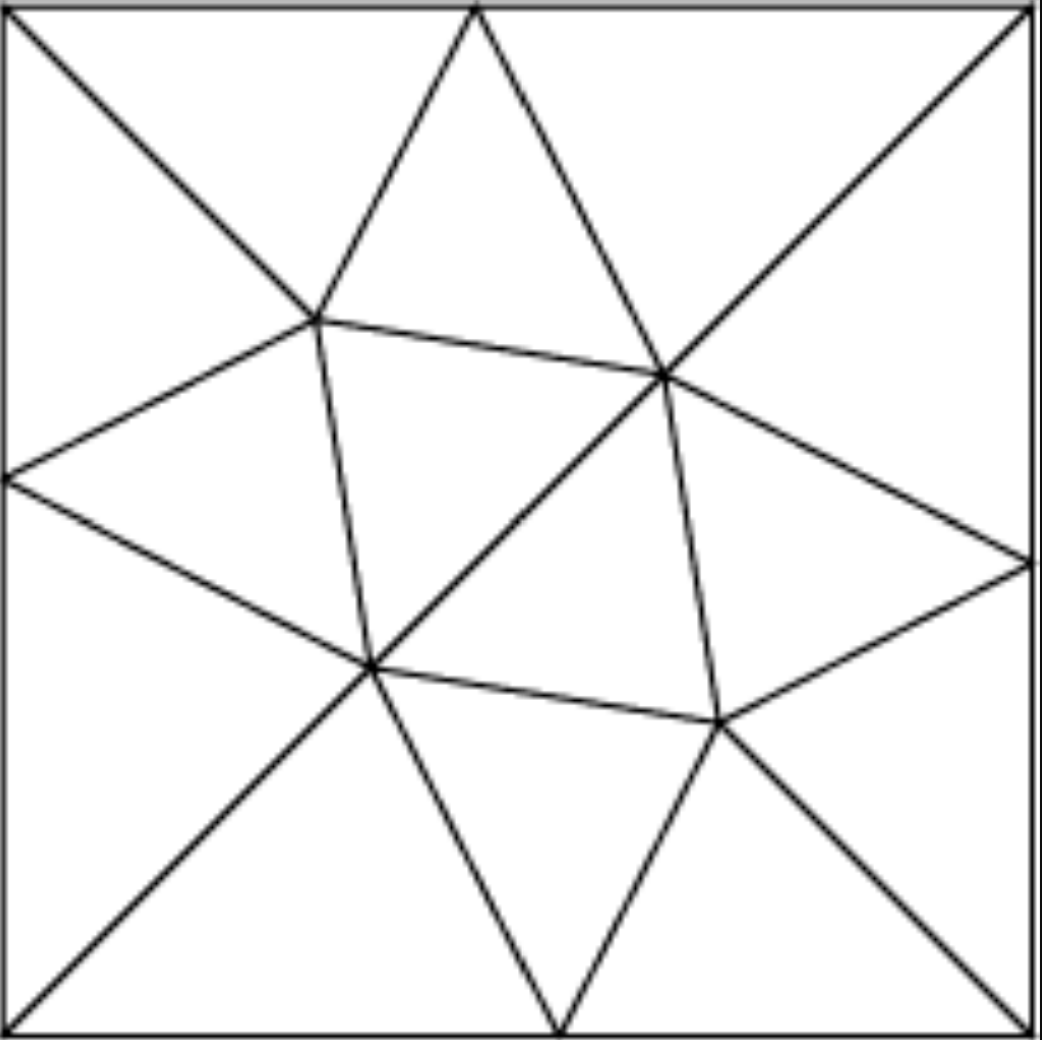
\includegraphics[scale=0.3]{tri-S^1_S^1.png}
% %     \centering
% %     \caption{triangulation of torus}
% % \end{figure}
% \begin{prop}
%     If $D \subseteq \mathbb{R}^n$ is a compact convex subset with nonempty interior, then $D$ is a closed $n$-cell 
%     and its interior is an open $n$-cell. In fact, given any point $p \in \operatorname{Int} D$, there exists a homeomorphism $F: \mathbb{B}^n \rightarrow D$ that sends 0 to $p, \mathbb{B}^n$ to Int $D$, and $\mathbb{S}^{n-1}$ to $\partial D$.
% \end{prop}
% \begin{defn}
%     An open $n$-cell is any topological space that is homeomorphic to the open unit ball $\mathbb{B}^n$, and a closed $n$-cell is any space homeomorphic to $\overline{\mathbb{B}}^n$.
% \end{defn}
% \begin{prop}
%     Thus every closed interval in $\mathbb{R}$ is a closed 1-cell; every compact region in the plane bounded by a regular polygon is a closed 2-cell; and a solid tetrahedron and 
%     a solid cube are closed 3-cells. 
%     By our conventions, any singleton is both a closed 0 -cell and an open 0-cell.
% \end{prop}







\chapter{Differential Manifold}

\section{Foundation}
\begin{defn}
    An $n$-dimensional topological manifold with boundary is a
    second-countable Hausdorff space $M$ in which every point has a neighborhood homeomorphic
    either to an open subset of $\mathbb{R}^n$ or to a (relatively)
    open subset of $\mathbb{H}^n$.
    An open subset $U \subseteq M$ together with a map $\varphi: U \rightarrow \mathbb{R}^n$ that is a homeomorphism onto
    an open subset of $\mathbb{R}^n$ or $\mathbb{H}^n$ will be called a chart for $M$,
    just as in the case of manifolds. When it is necessary to make the distinction, we will call $(U, \varphi)$ an interior chart if $\varphi(U)$ is an open subset of $\mathbb{R}^n$ (which includes the case of an open subset of $\mathbb{H}^n$ that does not intersect $\partial \mathbb{H}^n$ ), and a boundary chart if $\varphi(U)$ is an open subset of $\mathbb{H}^n$ such that $\varphi(U) \cap \partial \mathbb{H}^n \neq \varnothing$. A boundary chart whose image is a set of the form $B_r(x) \cap \mathbb{H}^n$ for some $x \in \partial \mathbb{H}^n$ and $r>0$ is called a coordinate half-ball.

    A point $p \in M$ is called an interior point of $M$ if it is in the domain of some interior chart. It is a boundary point of $M$ if it is in the domain of a boundary chart that sends $p$ to $\partial \mathbb{H}^n$. The boundary of $M$ (the set of all its boundary points) is denoted by $\partial M$; similarly, its interior, the set of all its interior points, is denoted by Int $M$.
\end{defn}
\begin{prop}[Topological Invariance of the Boundary]
    If $M$ is a topological manifold with boundary, then each point of $M$ is either a boundary point or an interior point, but not both. Thus $\partial M$ and $\operatorname{Int} M$ are disjoint sets whose union is $M$.
\end{prop}
\begin{prop}
    Let $M$ be a topological $n$-manifold with boundary.
    Int $M$ is an open subset of $M$ and a topological
    $n$-manifold without boundary and $\partial M$ is a closed subset of $M$ and a topological $n-1$ manifold without boundary.
\end{prop}
\begin{defn}
    To see how to define a smooth structure on a manifold
    with boundary, recall that a map from an arbitrary subset
    $A \subseteq \mathbb{R}^n$ to $\mathbb{R}^k$ is said to be smooth if in a neighborhood of each point of $A$ it admits an extension to a smooth map defined on an open subset of $\mathbb{R}^n$.
    Thus, if $U$ is an open subset of $\mathbb{H}^n$, a map $F: U \rightarrow \mathbb{R}^k$ is smooth
    if for each $x \in U$, there exists an open subset $\widetilde{U} \subseteq \mathbb{R}^n$ containing $x$
    and a smooth map $\widetilde{F}: \widetilde{U} \rightarrow \mathbb{R}^k$ that agrees with $F$ on $\widetilde{U} \cap \mathbb{H}^n$.
    If $F$ is such a map, the restriction of $F$ to $U \cap \operatorname{Int} \mathbb{H}^n$ is smooth in the usual sense.
    By continuity, all partial derivatives of $F$ at points of $U \cap \partial \mathbb{H}^n$ are determined by their values in Int $\mathbb{H}^n$, and therefore in particular are independent of the choice of extension.
\end{defn}
\begin{prop}
    $U$ is a open subset of $\bb{H}^n$. $F: U \rightarrow \mathbb{R}^k$ is smooth if and only
    if $F$ is continuous, $\left.F\right|_{U \cap \operatorname{Int} \mathbb{H}^n}$ is smooth, and the partial derivatives of $\left.F\right|_{U \cap \operatorname{Int} \mathbb{H}^n}$ of all orders have continuous extensions to all of $U$.
\end{prop}
\begin{defn}
    Let $M, N$ be smooth manifolds, and let
    $F: M \rightarrow N$ be any map. We say
    that $F$ is a smooth map if for every $p \in M$, there exist smooth charts $(U, \varphi)$ containing $p$ and $(V, \psi)$ containing $F(p)$ such that $F(U) \subseteq V$ and the composite map $\psi \circ F \circ$ $\varphi^{-1}$ is smooth from $\varphi(U)$ to $\psi(V)$. If $M$ and $N$ are smooth manifolds with boundary, smoothness of $F$ is defined in exactly the same way, with the usual understanding that a map whose domain is a subset of $\mathbb{H}^n$ is smooth if it admits an extension to
    a smooth map in a neighborhood of each point, and a map whose codomain is a subset of $\mathbb{H}^n$ is smooth if it is smooth as a map into $\mathbb{R}^n$.
\end{defn}
\begin{defn}
    Suppose $M$ is a topological space, and let $\mathcal{X}=\left(X_\alpha\right)_{\alpha \in A}$ be an arbitrary open cover of $M$, indexed by a set $A$. A partition of unity subordinate to $\mathcal{X}$ is an indexed family $\left(\psi_\alpha\right)_{\alpha \in A}$ of continuous functions $\psi_\alpha: M \rightarrow \mathbb{R}$ with the following properties:
    \begin{enu}
        \item $0 \leq \psi_\alpha(x) \leq 1$ for all $\alpha \in A$ and all $x \in M$.
        \item  $\operatorname{supp} \psi_\alpha \subseteq X_\alpha$ for each $\alpha \in A$.
        \item  The family of supports ( supp $\left.\psi_\alpha\right)_{\alpha \in A}$ is locally finite, meaning that every point has a neighborhood that intersects supp $\psi_\alpha$ for only finitely many values of $\alpha$.
        \item  $\sum_{\alpha \in A} \psi_\alpha(x)=1$ for all $x \in M$.
    \end{enu}
\end{defn}
\begin{theo}[Existence of Partitions of Unity]
    Suppose $M$ is a smooth manifold with or without boundary, and $\mathcal{X}=\left(X_\alpha\right)_{\alpha \in A}$ is any indexed open cover of $M$. Then there exists a smooth partition of unity subordinate to $\mathcal{X}$.
\end{theo}
\begin{defn}[Extension Lemma for Smooth Functions]
    Suppose $M$ is a smooth manifold with or without boundary, $A \subseteq M$ is a closed subset, and $f: A \rightarrow \mathbb{R}^k$ is a smooth function. For any open subset $U$ containing $A$, there exists a smooth function $\widetilde{f}: M \rightarrow \mathbb{R}^k$ such that $\left.\widetilde{f}\right|_A=f$ and $\operatorname{supp} \tilde{f} \subseteq U$.
\end{defn}




\begin{prop}[Smooth Manifold Chart Lemma]
    Let $M$ be a set, and suppose we are given a collection $\left\{U_\alpha\right\}$ of subsets of $M$ together with maps $\varphi_\alpha: U_\alpha \rightarrow \mathbb{R}^n$, such that the following properties are satisfied:
    \begin{enu}
        \item For each $\alpha, \varphi_\alpha$ is a bijection between $U_\alpha$ and an open subset $\varphi_\alpha\left(U_\alpha\right) \subseteq \mathbb{R}^n$.
        \item For each $\alpha$ and $\beta$, the sets $\varphi_\alpha\left(U_\alpha \cap U_\beta\right)$ and $\varphi_\beta\left(U_\alpha \cap U_\beta\right)$ are open in $\mathbb{R}^n$.
        \item Whenever $U_\alpha \cap U_\beta \neq \varnothing$, the $\operatorname{map} \varphi_\beta \circ \varphi_\alpha^{-1}: \varphi_\alpha\left(U_\alpha \cap U_\beta\right) \rightarrow \varphi_\beta\left(U_\alpha \cap U_\beta\right)$ is smooth.
        \item  Countably many of the sets $U_\alpha$ cover $M$.
        \item  Whenever $p, q$ are distinct points in $M$, either there exists some $U_\alpha$ containing both $p$ and $q$ or there exist disjoint sets $U_\alpha, U_\beta$ with $p \in U_\alpha$ and $q \in U_\beta$.
    \end{enu}
    Then $M$ has a unique smooth manifold structure such that each $\left(U_\alpha, \varphi_\alpha\right)$ is a smooth chart.
\end{prop}
\begin{lem}[existence of bump functions]
    If $M$ is a topological space, $A \subseteq M$ is a closed subset, and $U \subseteq M$ is an open subset containing $A$, a continuous function $\psi: M \rightarrow \mathbb{R}$ is
    called a bump function for $A$ supported in $U$ if $0 \leq \psi \leq 1$ on $M$, $\psi \equiv 1$ on $A$, and $\operatorname{supp} \psi \subseteq U$.

    Let $M$ be a smooth manifold with or without boundary. For any closed subset $A \subseteq M$ and any open subset $U$ containing $A$, there exists a smooth bump function for $A$ supported in $U$.
    \label{lemma:existence of bump function}
\end{lem}
\begin{exam}[smooth structure on vector space]
    Let $V$ be a finite-dimensional real vector
    space. Any norm on $V$ determines a topology,
    which is independent of the choice of norm. With this topology, $V$ is a topological $n$ manifold, and has a natural smooth structure defined as follows. Each (ordered) basis $\left(E_1, \ldots, E_n\right)$ for $V$ defines a basis isomorphism $E: \mathbb{R}^n \rightarrow V$ by
    $$
        E(x)=\sum_{i=1}^n x^i E_i .
    $$

    This map is a homeomorphism, so $\left(V, E^{-1}\right)$ is a chart. If $\left(\widetilde{E}_1, \ldots, \widetilde{E}_n\right)$ is any other basis and $\widetilde{E}(x)=\sum_j x^j \widetilde{E}_j$ is the corresponding isomorphism, then there is some invertible matrix $\left(A_i^j\right)$ such that $E_i=\sum_j A_i^j \widetilde{E}_j$ for each $i$. The transition map between the two charts is then given by $\widetilde{E}^{-1} \circ E(x)=\tilde{x}$, where $\tilde{x}=\left(\widetilde{x}^1, \ldots, \tilde{x}^n\right)$
    is determined by
    $$
        \sum_{j=1}^n \widetilde{x}^j \widetilde{E}_j=\sum_{i=1}^n x^i E_i=\sum_{i, j=1}^n x^i A_i^j \widetilde{E}_j .
    $$

    It follows that $\tilde{x}^j=\sum_i A_i^j x^i$. Thus, the map sending $x$ to $\tilde{x}$ is an invertible linear map and hence a diffeomorphism, so any two such charts are smoothly compatible. The collection of all such charts thus defines a smooth structure, called the standard smooth structure on $V$.
\end{exam}
\begin{defn}
    Let $M$ be a smooth $n$-manifold with or without boundary, and let $p \in M$. Then $T_p M$ is an n-dimensional vector space, and for any smooth chart $\left(U,\left(x^i\right)\right)$ containing $p$, the coordinate vectors $\partial /\left.\partial x^1\right|_p, \ldots, \partial /\left.\partial x^n\right|_p$ form a basis for $T_p M$.
\end{defn}
\section{Immersions and Submersions}
\begin{defn}
    A map between topological spaces is called proper if the preimage of every compact set is compact.
\end{defn}
\begin{lem}
    Let $Y$ be locally compact Hausdorff spaces. A proper continuous map $p: X \rightarrow Y$ is closed.
    \label{lemma:proper continuous, closed}
\end{lem}
\begin{prooff}
    Let $C \subset X$ be closed. Let $y \in Y-f(C)$.
    Since $Y$ is locally compact, $y$ has a neighborhood $V$ with compact closure.
    Since $f$ is proper, $f^{-1}(\bar{V})$ is compact in $X$.
    Let $E=C \cap f^{-1}(\bar{V})$, $E$ is compact; thus, $f(E)$ is compact.
    Since $Y$ is Hausdorff, $f(E)$ is closed. Let $\tilde{V}=V-f(E)$. $\tilde{V}$ is a neighborhood of $y$ disjoint from $f(C)$ as desired.
\end{prooff}
\begin{prop}[Sufficient Conditions for Properness]
    Suppose $X$ and $Y$ are topological spaces, and $F: X \rightarrow Y$ is a continuous map.
    \begin{enu}
        \item If $X$ is compact and $Y$ is Hausdorff, then $F$ is proper.
        \item If $F$ is a closed map with compact fibers, then $F$ is proper.
        \item If $F$ is a topological embedding with closed image, then $F$ is proper.
        \item If $Y$ is Hausdorff and $F$ has a continuous left inverse (i.e., a continuous map $G: Y \rightarrow X$ such that $\left.G \circ F=\operatorname{Id}_X\right)$, then $F$ is proper.
        \item If $F$ is proper and $A \subseteq X$ is a subset that is saturated with respect to $F$, then $\left.F\right|_A: A \rightarrow F(A)$ is proper.
    \end{enu}
\end{prop}
\begin{prop}
    Suppose $F: M \rightarrow N$ is a smooth map and $p \in M$. If $d F_p$ is surjective, then $p$ has a neighborhood $U$ such that $\left.F\right|_U$ is a submersion. If $d F_p$ is injective, then $p$ has a neighborhood $U$ such that $\left.F\right|_U$ is an immersion.
\end{prop}
\begin{prooff}
    If we choose any smooth coordinates for $M$ near $p$ and for $N$ near $F(p)$, either hypothesis means that Jacobian matrix of $F$ in coordinates has full rank at $p$. Since the set of $m \times n$ matrices of full rank is an open subset of $\mathrm{M}(m \times n, \mathbb{R})($ where $m=\operatorname{dim} M$ and $n=\operatorname{dim} N)$,
    so by continuity, the Jacobian of $F$ has full rank in some neighborhood of $p$.
\end{prooff}

\begin{theo}[Inverse Function Theorem for Manifolds]
    Suppose $M$ and $N$ are smooth manifolds, and $F: M \rightarrow N$ is a smooth map. If $p \in M$ is a point such that $d F_p$ is invertible, then there are connected neighborhoods $U_0$ of $p$ and $V_0$ of $F(p)$ such that $\left.F\right|_{U_0}: U_0 \rightarrow V_0$ is a diffeomorphism.
\end{theo}
\begin{coro}
    $F:M\rightarrow N$ is a local diffeomorphism if and only if it is both a smothh immersion and smooth submersion.
\end{coro}
\begin{coro}
    $F:M\rightarrow N$ smooth map, $\dim M=\dim N$. $F$ is diffeomorphism if and only if
    $F$ is bijective and both smooth immersion and submersion.
\end{coro}
\begin{theo}[Rank Theorem]
    Suppose $M$ and $N$ are smooth manifolds of dimensions $m$ and $n$, respectively, and $F: M \rightarrow N$ is a smooth map with constant rank $r$. For each $p \in M$ there exist smooth charts $(U, \varphi)$ for $M$ centered at $p$ and $(V, \psi)$ for $N$ centered at $F(p)$ such that $F(U) \subseteq V$, in which $F$ has a coordinate representation of the form
    $$
        \hat{F}\left(x^1, \ldots, x^r, x^{r+1}, \ldots, x^m\right)=\left(x^1, \ldots, x^r, 0, \ldots, 0\right) .
    $$

    In particular, if $F$ is a smooth submersion, this becomes
    $$
        \widehat{F}\left(x^1, \ldots, x^n, x^{n+1}, \ldots, x^m\right)=\left(x^1, \ldots, x^n\right),
    $$
    and if $F$ is a smooth immersion, it is
    $$
        \hat{F}\left(x^1, \ldots, x^m\right)=\left(x^1, \ldots, x^m, 0, \ldots, 0\right) \text {. }
    $$
\end{theo}
\begin{theo}[Global Rank Theorem]
    Let $M$ and $N$ be smooth manifolds, and suppose $F: M \rightarrow N$ is a smooth map of constant rank.
    \begin{enu}
        \item If $F$ is surjective, then it is a smooth submersion.
        \item If $F$ is injective, then it is a smooth immersion.
        \item If $F$ is bijective, then it is a diffeomorphism.
    \end{enu}
\end{theo}
\begin{defn}[embedded submanifold]
    Suppose $M$ is a smooth manifold with or without boundary. An embedded submanifold of $M$ is a subset $S \subseteq M$ that is a manifold (without boundary) in the subspace topology, endowed with a smooth structure with respect to which the inclusion map
    $S \hookrightarrow M$ is a smooth embedding.

    If $S$ is an embedded submanifold of $M$, the $\operatorname{difference} \operatorname{dim} M-\operatorname{dim} S$ is called the codimension of $S$ in $M$, and the containing manifold $M$ is called the ambient manifold for $S$. An embedded hypersurface is an embedded submanifold of codimension 1 . The empty set is an embedded submanifold of any dimension.
\end{defn}
\begin{theo}[smooth structure of boundary]
    Theorem 5.11. If $M$ is a smooth n-manifold with boundary,
    then with the subspace topology, $\partial M$ is a topological $(n-1)$-dimensional manifold (without boundary), and has a unique smooth structure such that it is a properly embedded submanifold of $M$.
\end{theo}
\begin{prop}
    Suppose $M$ is a smooth manifold with or without boundary and $S \subseteq M$ is an embedded submanifold. Then $S$ is properly embedded if and only if it is a closed subset of $M$.
\end{prop}
\begin{defn}
    If $M$ is a smooth manifold with boundary and
    $p \in \partial M$, it is intuitively evident that
    the vectors in $T_p M$ can be separated into three classes: those tangent to the boundary, those pointing inward, and those pointing outward. Formally, we make the following definition. If $p \in \partial M$, a vector $v \in T_p M-T_p \partial M$ is said to be inwardpointing if for some $\varepsilon>0$ there exists a smooth curve $\gamma:[0, \varepsilon) \rightarrow M$ such that $\gamma(0)=p$ and $\gamma^{\prime}(0)=v$, and it is outward-pointing if there exists such a curve whose domain is $(-\varepsilon, 0]$.
    The following proposition gives another characterization of inward-pointing and outward-pointing vectors, which is usually much easier to check.
\end{defn}

\blue{For the following results, manifolds mentioned are all without boundary.}
\begin{defn}[regular submanifold/local slice criterion]
    A subset $S$ of a manifold(or satisfying local slice criterion) $N$ of dimension $n$ is a regular submanifold of dimension $k$ if for every $p \in S$
    there is a coordinate neighborhood $(U, \phi)=\left(U, x^1, \ldots, x^n\right)$ of $p$ in the maximal atlas of $N$ such that $U \cap S$ is defined by the vanishing of $n-k$ of the coordinate functions. By renumbering the coordinates, we may assume that these $n-k$ coordinate functions are $x^{k+1}, \ldots, x^n$.
    We call such a chart $(U, \phi)$ in $N$ an adapted chart relative to $S$. On $U \cap S, \phi=$ $\left(x^1, \ldots, x^k, 0, \ldots, 0\right)$. Let
    $$
        \phi_S: U \cap S \rightarrow \mathbb{R}^k
    $$
    be the restriction of the first $k$ components of $\phi$ to $U \cap S$, that is, $\phi_S=\left(x^1, \ldots, x^k\right)$.
\end{defn}
\begin{prop}
    Let $S$ be a regular submanifold of $N$ of dimension $k$, then $S$ with subspace topology is a topological manifold of dimension $k$.
    And there's a unique smooth structure on $S$ such that $S$ is a $k$-dimensional embedded submanifold of $M$.
    \label{proposition:smooth structure of S}
\end{prop}
\begin{prooff}
    Clearly, $S$ is a $k$-dimensional topological manifold.
    It's easy to check that for the collection of all adapted charts $\bbrace{U,\phi}$ relative to $S$ ,
    $\bbrace{U\cap S,\phi_S}$ form an atlas of $S$.

    Conversely, if $F:S\rightarrow M$ is a smooth embedding, there's $(U,\phi)$ and $(V,\psi)=(V,y^1,\dots,y^m)$ such that
    $\psi \circ F\circ \phi^{-1}$ is given by
    \begin{equation*}
        (x^1,\dots,x^k)\mapsto (x^1,\dots,x^k,0,\dots,0)\in \bb{R}^m
    \end{equation*}
    Let $V_1=\psi^{-1}(\psi(V)\cap \phi(U)\times \bb{R}^{n-k})$ and $U=S\cap W$, $W$ open in $M$.
    We have $U=S\cap W=S\cap (V_1\cap W)=\bbrace{v\in V_1\cap W: y^{k+1}(v)=\dots=y^{m}(v)=0}$.
    Hence local chart of $S$ is given by adapted chart, which implies the smooth structure on $S$
    is unique.
\end{prooff}
% \begin{defn}
%     A level set of a map $F: N \rightarrow M$ is a subset
%     $$
%         F^{-1}(\{c\})=\{p \in N \mid F(p)=c\}
%     $$
%     for some $c \in M$.
%     The value $c \in M$ is called the level of the level set $F^{-1}(c)$.
%     Define that $c$ is a regular value of $F$ if and only if either $c$ is not in the image of $F$ or at every point $p \in F^{-1}(c)$, the differential $F_{*, p}: T_p N \rightarrow T_{F(p)} M$ is surjective.
%     The inverse image $F^{-1}(c)$ of a regular value $c$ is called a regular level set.
% \end{defn}
\begin{theo}[Constant-rank level set theorem]
    Let $M$ and $N$ be smooth manifolds, and
    let $\Phi: M \rightarrow N$ be a smooth map with constant rank $r$.
    Each level set of $\Phi$ is a properly embedded submanifold of codimension $r$ in $M$.
    \label{theorem:Constant-rank level set theorem}
\end{theo}
\begin{prooff}
    Notice that $\Phi^{-1}(c)$ is regular submanifold and closed submanifold, hence it can be given a unique smooth structure such that
    $\Phi^{-1}(c)$ is a properly embedded submanifold of codimension $r$ in $M$.
\end{prooff}
\begin{prop}
    Let $M$ and $N$ be smooth manifolds, and
    let $\Phi: M \rightarrow N$ be a smooth map with constant rank $r$.
    Let $S$ be a level set of $\Phi$ at $c\in N$, then by Theorem~\ref{theorem:Constant-rank level set theorem}, $S$ be a properly embedded submanifold of $M$.
    We have an exact sequence
    \begin{equation*}
        0\rightarrow T_pS\rightarrow T_pM\rarr{(\text{d}\Phi)_p} T_cN
    \end{equation*}
    for all $p$ in $S$.
\end{prop}
\section{Vector Field}
\begin{prop}
    Let $M$ be a smooth manifold with or without boundary, and let $X: M \rightarrow T M$ be a rough vector field. The following are equivalent:
    \begin{enu}
        \item $X$ is smooth.
        \item For every $f \in C^{\infty}(M)$, the function $X f$ is smooth on $M$.
    \end{enu}
\end{prop}
\begin{lem}[Extension of vector field]
    Let $M$ be a smooth manifold with or without boundary, and let $A \subseteq M$ be a closed subset. Suppose $X$ is a smooth vector field along A. Given any open subset $U$ containing $A$, there exists a smooth global vector field $\tilde{X}$ on $M$ such that $\left.\tilde{X}\right|_A=X$ and $\operatorname{supp} \tilde{X} \subseteq U$.
    \label{lemma:extension of vector field}
\end{lem}
\begin{defn}
    We can also consider mixed $(k,m)$-tensors on $V$, that is, multilinear functions defined on the product $V \times \cdots \times V \times V^* \times \cdots \times V^*$ of $k$ copies of $V$ and $m$ copies of $V^*$. A $(k, m)$-tensor is then $k$ times covariant and $m$ times contravariant on $V$. The space of all $(k, m)$-tensors on $V$ is denoted by $\mathcal{T}^{k, m}\left(V^*, V\right)$.
\end{defn}
\begin{defn}
    A $(k, m)$-tensor field is a map that to each point $p \in M$ assigns a tensor $T \in \mathcal{T}^{k, m}\left(T_p^* M, T_p M\right)$.
\end{defn}
\begin{defn}
    The space of $(k, m)$-tensor fields is clearly a vector space,
    since linear combinations of $(k, m)$-tensors are still $(k, m)$-tensors.
    If $W$ is a coordinate neighborhood of $M$, we know that $\left\{\left(d x^i\right)_p\right\}$ is a basis for $T_p^* M$ and that $\left\{\left(\frac{\partial}{\partial x^i}\right)_p\right\}$ is a basis for $T_p M$. Hence, the value of a $(k, m)$-tensor field $T$ at a point $p \in W$ can be written as the tensor
    $$
        T_p=\sum a_{i_1 \cdots i_k}^{j_1 \cdots j_m}(p)\left(d x^{i_1}\right)_p \otimes \cdots \otimes\left(d x^{i_k}\right)_p \otimes\left(\frac{\partial}{\partial x^{j_1}}\right)_p \otimes \cdots \otimes\left(\frac{\partial}{\partial x^{j_m}}\right)_p
    $$
    where the $a_{i_1 \ldots i_k}^{j_1 \ldots j_m}: W \rightarrow \mathbb{R}$ are functions which at
    each $p \in W$ give us the components of $T_p$ relative to these bases of $T_p^* M$ and $T_p M$.
    Just as we did with vector fields, we say that a tensor field is smooth if all these functions are smooth for all coordinate systems of the maximal atlas. Again, we \blue{only need to consider} the coordinate systems of an atlas, since all overlap maps are differentiable.
\end{defn}



\begin{prop}
    $M$ is a smooth manifold with or without boundary, there's a one-to-one bijection between
    vector field $\mathfrak{X}(M)$ on $M$ and linear operaters $C^{\infty}(M)\rightarrow C^{\infty}(M)$ satisfying Leibniz rule.
    \label{correspondence:vector field and Der}
\end{prop}
\begin{prop}
    Given two differentiable vector fields $X, Y \in \mathfrak{X}(M)$ on a smooth manifold $M$(with or without boundary), there exists a unique differentiable vector field $Z \in \mathfrak{X}(M)$ such that
    $$
        Z \cdot f=(X \circ Y-Y \circ X) \cdot f
    $$
    for every differentiable function $f \in C^{\infty}(M)$. And we denote $Z$ by $[X,Y]$.
\end{prop}
\begin{prooff}
    It suffice to check $[X,Y]$ satisfies Leibniz rule and use Proposition~\ref{correspondence:vector field and Der}
\end{prooff}
\begin{theo}[Coordinate Formula for the Lie Bracket]
    Let $X, Y$ be smooth vector fields on a smooth manifold $M$ with or without boundary, and let
    $$
        X=\sum_{i=1}^nX^i \frac{\partial}{\partial x^i}
    $$
    and
    $$
        Y=\sum_{i=1}^nY^i \frac{\partial}{\partial x^i}
    $$
    be the coordinate expressions for $X$ and $Y$ in terms of some smooth local coordinates $\left(U,x^1,\dots,x^n\right)$ for $M$. Then $[X, Y]$ has the following coordinate expression:
    $$
        [X, Y]=\sum_{i=1}^n\sum_{j=1}^n\left(X^i \frac{\partial Y^j}{\partial x^i}-Y^i \frac{\partial X^j}{\partial x^i}\right) \frac{\partial}{\partial x^j}
    $$
\end{theo}
\begin{prop}
    Given $X, Y, Z \in \mathfrak{X}(M)$, we have:
    \begin{enu}
        \item Bilinearity: for any $\alpha, \beta \in \mathbb{R}$,
        $$
            \begin{aligned}
                 & {[\alpha X+\beta Y, Z]=\alpha[X, Z]+\beta[Y, Z]} \\
                 & {[X, \alpha Y+\beta Z]=\alpha[X, Y]+\beta[X, Z]}
            \end{aligned}
        $$
        \item Antisymmetry:
        $$
            [X, Y]=-[Y, X]
        $$
        \item Jacobi identity:
        $$
            [[X, Y], Z]+[[Y, Z], X]+[[Z, X], Y]=0 ;
        $$
    \end{enu}
\end{prop}
\begin{defn}
    A vector space $V$ equipped with an antisymmetric bilinear map $[\cdot, \cdot]$ : $V \times V \rightarrow V$ (called a Lie bracket) satisfying the Jacobi identity is called a Lie algebra. A linear map $F: V \rightarrow W$ between Lie algebras
    is called a Lie algebra homomorphism if $F\left(\left[v_1, v_2\right]\right)=\left[F\left(v_1\right), F\left(v_2\right)\right]$ for all $v_1, v_2 \in V$. If $F$ is bijective then it is called a Lie algebra isomorphism.
\end{defn}
\begin{lem}[Extension Lemma for Vector Fields on Submanifolds]
    $M$ is a smooth manifold with or without boundary and $S \subseteq M$ is an embedding submanifold.
    Given $X \in \mathfrak{X}(S)$, then there is a smooth vector field $Y$ on a
    neighborhood of $S$ in $M$ such that $X=\left.Y\right|_S$.
    \label{lemma:Extension Lemma for Vector Fields on Submanifolds}
\end{lem}
\section{Differential form}


\begin{defn}
    Let $\left(U, x^1, \ldots, x^n\right)$ be a chart on a manifold $M$.
    $A$-form $\omega=\sum a_I d x^I$ on $U$ is smooth(continous) if and only if the coefficient functions $a_I$ are all smooth(continous) on $U$.
\end{defn}
\begin{defn}[Characterization of a smooth $k$-form]
    Let $\omega$ be a $k$-form on a manifold $M$. The following are equivalent:

    (1) The $k$-form $\omega$ is $C^{\infty}$ on $M$.

    (2) The manifold $M$ has an atlas such that on every chart $(U, \phi)=\left(U, x^1, \ldots, x^n\right)$ in the atlas, the coefficients $a_I$ of $\omega=\sum a_I d x^I$ relative to the coordinate frame $\left\{d x^I\right\}_{I \in \mathcal{J}_{k, n}}$ are all $C^{\infty}$.

    (3) On every chart $(U, \phi)=\left(U, x^1, \ldots, x^n\right)$ on $M$, the coefficients $a_I$ of $\omega=\sum a_I d x^I$ relative to the coordinate frame $\left\{d x^I\right\}_{I \in \mathcal{J}_{k, n}}$ are all $C^{\infty}$.

    (4) For any $k$ smooth vector fields $X_1, \ldots, X_k$ on $M$, the function $\omega\left(X_1, \ldots, X_k\right)$ is $C^{\infty}$ on $M$.
\end{defn}
\begin{rema}
    (1), (2) and (3) in above conditions are also equivalent if we replace "smooth" by "continuous".
\end{rema}
\begin{defn}[pullback of differential form]
    Now suppose $F: N \rightarrow M$ is a $C^{\infty}$ map of manifolds. At each point $p \in N$, the differential
    $$
        F_{*, p}: T_p N \rightarrow T_{F(p)} M
    $$
    is a linear map of tangent spaces, and so there is a pullback map
    $$
        \left(F_{*, p}\right)^*: A_k\left(T_{F(p)} M\right) \rightarrow A_k\left(T_p N\right) .
    $$

    If $\omega$ is a $k$-form on $M$, then its pullback $F^* \omega$ is the $k$-form on $N$ defined pointwise by $\left(F^* \omega\right)_p= \left(F_{*, p}\right)^*\left(\omega_{F(p)}\right)$ for all $p \in N$.
\end{defn}



\section{Orientation}
\begin{defn}
    Let $V$ be a finite dimensional vector space and consider two ordered bases $\beta=$ $\left\{b_1, \ldots, b_n\right\}$ and $\beta^{\prime}=\left\{b_1^{\prime}, \ldots, b_n^{\prime}\right\}$.
    There is a unique linear transformation $S$ : $V \rightarrow V$ such that $b_i^{\prime}=S b_i$ for every $i=1, \ldots, n$. We say that the two bases are equivalent if $\operatorname{det} S>0$. This defines an equivalence relation that divides the set of all ordered bases of $V$ into two equivalence classes. An orientation for $V$ is an assignment of a positive sign to the elements of one equivalence class and a negative sign to the elements of the other. The sign assigned to a basis is called its orientation and the basis is said to be positively oriented or negatively oriented according to its sign.
    It is clear that there are exactly two possible orientations for $V$.

    We always take $[e_1,\dots,e_n]$ as an representative to the positive orientation of $\bb{R}^n$.
\end{defn}
\begin{defn}
    An isomorphism $A: V \rightarrow W$ between two oriented vector spaces
    carries equivalent ordered bases of $V$ to equivalent ordered bases of $W$.
    Under this case, isomorphism $A$ is said to be orientation-preserving.

    An orientation of a smooth manifold consists of a choice of orientations
    for all tangent spaces $T_p M$.
    If $\operatorname{dim} M=n \geq 1$, these orientations have to fit
    together smoothly, meaning that for each point $p \in M$ there exists a local chart $(U,\varphi)=(U,x^1,\dots,x^n)$ around $p$ such that
    $$
        T_pM\rightarrow \bb{R}^n,\quad \sum a_i\frac{\partial}{\partial x^i}\mapsto (a_1,\dots,a_n)
    $$
    is order-preserving.
\end{defn}
\begin{prop}
    If a smooth manifold $M$ is connected and orientable then it admits precisely two orientations.
\end{prop}
\begin{prooff}

\end{prooff}
\begin{prop}
    A smooth manifold $M$ is orientable if and only if
    there exists an atlas $\mathcal{A}=\left\{\left(U_\alpha, \varphi_\alpha\right)\right\}$
    for which all the overlap maps $\varphi_\beta \circ \varphi_\alpha^{-1}$ has positive Jacobi determinant for all $p\in \varphi_{\alpha}(U_{\alpha}\cap U_{\beta})$.
\end{prop}
\begin{prooff}
    For every $p\in M$, take $(U_{\alpha},\varphi_{\alpha})\in \mathcal{A}$ such that $p\in U_{\alpha}$. Fix an orientation on $T_p M$ to be the equivalent class of the basis $$(\frac{\partial}{\partial x_1}\bigg|_p,\frac{\partial}{\partial x_2}\bigg|_p,\dots,\frac{\partial}{\partial x_n}\bigg|_p)$$, then the map
    \begin{equation*}
        p\mapsto [(\frac{\partial}{\partial x_1}\bigg|_p,\frac{\partial}{\partial x_2}\bigg|_p,\dots,\frac{\partial}{\partial x_n}\bigg|_p)]
    \end{equation*}
    is well-defined and gives an orientation on $M$.
\end{prooff}
\begin{prop}
    $M$ is a connected manifold, $M$ is orientable if and only if $M$ has a nowhere-vanishing $n$-form.
\end{prop}
\begin{prooff}
    Suppose $(X_1,\dots,X_n)$ is an orientable on $M$, for all $p\in M$, there exists a parameterization $(U,\varphi)=(U,x^1,\dots,x^n)$ around $p$ such that
    $$
        T_pM\rightarrow \bb{R}^n,\quad \sum a_i\frac{\partial}{\partial x^i}\mapsto (a_1,\dots,a_n)
    $$
    is order-preserving.
    Hence $\text{d}x^1\wedge\dots \text{d}x^n(X_1,\dots,X_n)>0$ for all $p\in U$. For all $p$, consider such local chart, we get an atlas
    $\mathcal{A}=\left\{\left(U_\alpha, \varphi_\alpha\right)\right\}$. Consider $\bbrace{\rho_{\alpha}}_{\alpha\in A}$ be partition of union.

    Let
    \begin{equation*}
        \omega_p= \sum_{\rho_{\alpha}(p)\neq 0} \rho_{\alpha}(p)\text{d}x^1_{\alpha}\wedge\dots \text{d}x^n_{\alpha}
    \end{equation*}
    Then $\omega(X_1,\dots,X_n)\neq 0$, which implies $\omega $ is a nowhere-vanishing $n$-form.

    Conversely, consider $\omega$ be a nowhere-vanishing $n$-form, take a connected local chart $(U,x^1,\dots,x^n)$ and assume that $\omega(\frac{\partial}{\partial x_1},\frac{\partial}{\partial x_2},\dots,\frac{\partial}{\partial x_n})>0$, otherwise we can replace $x^1$ by $-x^1$.
\end{prooff}
\begin{defn}
    Two oriented atlas $\bbrace{(U_{\alpha},\phi_{\alpha})}_{\alpha\in A}$ and $\bbrace{V_{\beta},\psi_{\beta}}_{\beta}$ on a manifold $M$ are said to be equivalent if the transition functions
    \begin{equation*}
        \phi_{\alpha}\circ\psi_{\beta}^{-1}:\psi_{\beta}^{-1}(U_{\alpha}\cap V_{\beta})\rightarrow \phi_{\beta}^{-1}(U_{\alpha}\cap V_{\beta})
    \end{equation*}
    have positive Jacobian determinant for all $\alpha,\beta$.
\end{defn}
\begin{prop}
    $M$ is an oriented connected manifold, then
    there's a ono-to-one correspondence between
    equivanlece classes of oriented atlases on $M$.
\end{prop}
\begin{prooff}
    Two oriented atlas $\bbrace{(U_{\alpha},\phi_{\alpha})}_{\alpha\in A}$ and $\bbrace{V_{\beta},\psi_{\beta}}_{\beta}$
    on a manifold $M$ are equivalent, they give the same orientations on $M$.

    Two oriented atlas $\bbrace{(U_{\alpha},\phi_{\alpha})}_{\alpha\in A}$ and $\bbrace{V_{\beta},\psi_{\beta}}_{\beta}$
    on a manifold $M$ are inequivalent, they give different orientations on $M$.

    And also notice that if $\bbrace{(U_{\alpha},x^1,\dots,x^n)}_{\alpha\in A}$ is an oriented atalas, then
    $\bbrace{(U_{\alpha},-x^1,\dots,x^n)}_{\alpha\in A}$ is also an oriented atalas which is not equivalent to previous one.
\end{prooff}
\begin{theo}
    If $\omega$ is a nowhere-vanishing $n$-form(not need to be smooth) on a connected oriented manifold $M$, $\bbrace{(U_{\alpha},\phi_{\alpha})}_{\alpha\in A}$ is an oriented atlas. For every $p\in M$ and every coordinate neighborhood $(U,\phi)=(u,x^1,\dots,x^n)$ of $p$, $\omega$ can be
    written as $w(q)=f(q)dx^1\wedge \dots dx^n, q\in U$. Define
    \begin{align}
        g(p)=
        \begin{cases}
            1  & \text{if} \quad f(p)>0 \\
            -1 & \text{if} \quad f(p)<0
        \end{cases}
    \end{align}
    g is well-defined since  the atlas is oriented. We have $g$ is constant function on $M$.
\end{theo}
\section{Integration on manifold}
Let $M$ be a oriented manifold $M$ with an oriented atlas $\bbrace{(U_{\alpha},\phi_{\alpha})}_{\alpha\in A}$, $\omega$ be a compactly support continuous $n$-form on $M$.
Suppose $\text{supp}\,\omega\subset U_{\alpha}$ and $(U_{\alpha},\phi_{\alpha})=(u,x^1,\dots,x^n)$.Then $\omega$ has a local expression on $U_{\alpha}$ written as $w(q)=f(q)dx^1\wedge \dots dx^n, q\in U_{\alpha}$, define
\begin{equation}
    \int_{M}\omega=\int_{\phi_{\alpha}(U_{\alpha})}f\circ\phi_{\alpha}^{-1}
\end{equation}
Notice that this definition is independent of the choice of the chart in oriented atlas since if $(U_{\beta},\phi_{\beta})=(U_{\alpha},y^1,\dots,y^n)$ is another chart in oriented atlas such that
$\text{supp}\,\omega\subset U_{\beta}$
\begin{align*}
    \int_{M}\omega & =\int_{\phi_{\alpha}(U_{\alpha})}f\circ\phi_{\alpha}^{-1}                                                             &                                        \\
                   & =\int_{\phi_{\alpha}(U_{\alpha}\cap U_{\beta})}f\circ\phi_{\alpha}^{-1}                                               &                                        \\
                   & =\int_{\phi_{\beta} (U_{\alpha}\cap U_{\beta})}f\circ\phi_{\beta}^{-1}|\det D_x(\phi_{\alpha}\circ\phi_{\beta}^{-1})| & (\text{$D_x$ is Jacobian matrix})      \\
                   & =\int_{\phi_{\beta} (U_{\alpha}\cap U_{\beta})}f\circ\phi_{\beta}^{-1} \det D_x(\phi_{\alpha}\circ\phi_{\beta}^{-1})  & (\text{proposition of oriented atlas}) \\
\end{align*}
Notice that the last identity agrees with the integration defined by $(U_{\beta},\phi_{\beta})=(U_{\alpha},y^1,\dots,y^n)$, hence the integration is well-defined.

In general, if $\omega$ is arbitrary compactly supported $n$-form on $M$, we need a lemma.
\begin{lem}
    Let $\bbrace{\rho_{\alpha}}_{\alpha\in A}$ be a collection of functions on $M$ and $\omega$ a continous $k$-form on $M$ with compact support. If the collection $\bbrace{\rho_{\alpha}:M\rightarrow\bb{R}}_{\alpha\in A}$
    of supports is locally finite, then $\rho_{\alpha}\omega\equiv 0$ for all but finte $\alpha$.
\end{lem}
\begin{prooff}
    Let $p\in \text{supp}\,\omega$. Since $\text{supp}\,\rho_{\alpha}$ is locally fnite, there is a neighborhood $W_p$ of $p$ in M htat intersects only finitely many of the sets $\text{supp}\,\rho_{\alpha}$. The collection
    $\bbrace{W_p|p\in M}$ is an open covering of $\text{supp}\,\omega$. Take a finite subcovering $W_1,\dots,W_p$, then we have only finte many $\text{supp}\,\rho_{\alpha}$ intersects $\bigcup_{i=1}^n W_i$. In partical, $\rho_{\alpha}\omega\equiv 0$ for all but finte $\alpha$.
\end{prooff}

Let $\bbrace{\rho_{\alpha}}_{\alpha\in A}$ to be the smooth
partition of unity dominated to oriented atlas $\bbrace{(U_{\alpha},\phi_{\alpha})}_{\alpha\in A}$.
Let $U_i,\, i=1,\dots,n$ be all the charts such that $\rho_{\alpha}\omega$ are nontrival.
Define
\begin{equation*}
    \int_{M}\omega=\sum_{i=1}^n\int_M\rho_i w
\end{equation*}
where the integration of $\rho_i w$ on $M$ is belong to the case we have already defined.

To check the above identity is well defined, let $\bbrace{V_{\beta},\psi_{\beta}}_{\beta}$ be another oriented atlas equivalent to $\bbrace{(U_{\alpha},\phi_{\alpha})}_{\alpha\in A}$.
$\bbrace{\chi_{\beta}}_{\beta}$ be the smooth partition of unity of $M$ dominated by $\bbrace{V_{\beta},\psi_{\beta}}_{\beta}$
and let $V_i,\, i=1,\dots m$ be all the charts such that $\chi_{\alpha}\omega$ are nontrival.
Notice that
\begin{equation*}
    \sum_{i=1}^n\int_M\rho_i w=\sum_{i=1}^n\int_M\rho_i\sum_{j=1}^m \chi_j w=\sum_{i=1}^n \sum_{j=1}^m \int_M \rho_i \chi_j w
\end{equation*}

Since $\bbrace{V_{\beta},\psi_{\beta}}_{\beta}$ is equivalent to $\bbrace{(U_{\alpha},\phi_{\alpha})}_{\alpha\in A}$,
the integration of $\rho_i \chi_j \omega$ defined by $U_i$ is identical to the integretion defined by $V_j$.
Hence $\int_M \omega $ is well-defined.

Now we assume $M$ is connected and oriented.

Since there's a smooth nowhere-vanishing $n$-form $\omega$ such that the coefficient of the local expression under the given oriented atlas is always positive.
Take a function $f$ in the space of compactly supported function $C_c(M)$, then $f\omega$ is a compactly supported continous $n$-form. Hence the linear functional
\begin{equation*}
    I:f\rightarrow \int_M f\omega
\end{equation*}
is a positive linear functional on $C_c(M)$. By Riesz Representation Theroem, there's a Radon measure $\mu$ on $M$ such that
\begin{equation*}
    I(f)=\int f \dd \mu
\end{equation*}
for all $f\in C_c(M)$.
% \begin{prop}
%     Let $M$ be an $n$-dimensional differentiable manifold. A subset $N \subset M$ is said to have zero measure if the sets $\varphi_\alpha^{-1}(N) \subset U_\alpha$ have zero measure for every parameterization $\varphi_\alpha: U_\alpha \rightarrow M$ in the maximal atlas.

%     (1) Prove that in order to show that $N \subset M$ has zero measure it suffices to check that the sets $\varphi_\alpha^{-1}(N) \subset U_\alpha$ have zero measure for the parameterizations in an arbitrary atlas.

%     (2) Suppose that $M$ is oriented. Let $\omega \in \Omega^n(M)$ be compactly supported and let $W=\varphi(U)$ be a coordinate neighborhood such that $M \backslash W$ has zero measure. Show that
%     $$
%         \int_M \omega=\int_U \varphi^* \omega,
%     $$
% \end{prop}
% \begin{prooff}

% \end{prooff}




\section{Affine Connection}
\begin{defn}
    A tensor $g \in \mathcal{T}^2\left(T_p^* M\right)$ is said to be

    (1) symmetric if $g(v, w)=g(w, v)$ for all $v, w \in T_p M$;

    (2) nondegenerate if $g(v, w)=0$ for all $w \in T_p M$ implies $v=0$;

    (3) positive definite if $g(v, v)>0$ for all $v \in T_p M \backslash\{0\}$.

    A covariant 2-tensor field $g$ is said to be symmetric, nondegenerate or positive definite if $g_p$ is symmetric, nondegenerate or positive definite for all $p \in M$. If $x: V \rightarrow \mathbb{R}^n$ is a local chart, we have
    $$
        g=\sum_{i=1}^n\sum_{j=1}^n g_{i j} d x^i \otimes d x^j
    $$
    in $V$, where
    $$
        g_{i j}=g\left(\frac{\partial}{\partial x^i}, \frac{\partial}{\partial x^j}\right) .
    $$

    It is easy to see that $g$ is symmetric, nondegenerate or positive definite if and only if the matrix $\left(g_{i j}\right)$ has these properties.
\end{defn}
\begin{defn}
    A Riemannian metric on a smooth manifold $M$ is a symmetric positive definite smooth covariant 2-tensor field $g$. A smooth manifold $M$ equipped with a Riemannian metric $g$ is called a Riemannian manifold, and is denoted by $(M, g)$.
\end{defn}
\begin{defn}
    An oriented manifold is an orientable manifold together
    with a choice of an orientation. A map $F: M \rightarrow N$ between two oriented manifolds with
    the same dimension is said to be orientation-preserving if $F_{*,p}$ is orientation-preserving at all points $p \in M$.

    The Riemannian metric is also denoted by form of inner product $p\mapsto 	\left \langle \,,\, \right \rangle_p$.
\end{defn}
\begin{prop}
    Let $(N, g)$ be a Riemannian manifold and $F: M \rightarrow N$ an immersion($F_{*,p}$ is injective for all $p\in M$).
    Then for $u,v\in T_pM$, define $(u,v)_p=(F_{*,p}(u), F_{*,p}(v))$ is a Riemannian metric in $M$ (called the induced metric).
\end{prop}
\begin{exam}
    The standard metric on
    $$
        S^n=\left\{x \in \mathbb{R}^{n+1} \mid\|x\|=1\right\}
    $$
    is the metric induced on $S^n$ by the Euclidean metric on $\mathbb{R}^{n+1}$. A chart $(U,\varphi)=(U,x^1,\dots,x^n)$
    $$
        U=\left\{x \in S^n \mid x^{n+1}>0\right\}
    $$
    and
    $$
        \varphi^{-1}\left(x_1, \ldots, x_n\right)=\left(x_1, \ldots, x_n, \sqrt{1-\left(x_1\right)^2-\cdots-\left(x_n\right)^2}\right), (x_1,\dots,x_n)\in B(0,1)\subset \bb{R}^n
    $$
    and the corresponding coefficients of the metric tensor are
    $$
        g_{i j}=\left\langle\frac{\partial}{\partial x^i}, \frac{\partial }{\partial x^j}\right\rangle=\delta_{i j}+\frac{x^i x^j}{1-\left(x^1\right)^2-\cdots-\left(x^n\right)^2} .
    $$
\end{exam}
% \begin{exam}[Volume form on Sphere]
%     Consider $n$-form on $\bb{R}^{n+1}$
%     \begin{equation*}
%         \omega=\sum_{i=1}^{n+1} (-1)^{i-1}x_i \dd x_1 \wedge \dots\wedge \dd x_{i-1}\wedge \dots  \wedge \dd x_{i+1}\dots \wedge \dd x_{n+1}
%     \end{equation*}
%     and the inclution map $i:S^n \hookrightarrow \bb{R}^{n+1}$. The embedding map $i$ induce a Riemannian metric on $S^n$ and the pullback of $\omega$ by $i$ is the volume form on $S^n$. We denote it by Vol $S^n$.
% \end{exam}
\begin{defn}
    Let $M$ be a differentiable manifold. An affine connection on $M$ is a map $\nabla: \mathfrak{X}(M) \times \mathfrak{X}(M) \rightarrow \mathfrak{X}(M)$ such that

    (1) $\nabla_{f X+g Y} Z=f \nabla_X Z+g \nabla_Y Z$;

    (2) $\nabla_X(Y+Z)=\nabla_X Y+\nabla_X Z$

    (3) $\nabla_X(f Y)=(X \cdot f) Y+f \nabla_X Y$
    for all $X, Y, Z \in \mathfrak{X}(M)$ and $f, g \in C^{\infty}(M, \mathbb{R})$ (we write $\nabla_X Y:=\nabla(X, Y)$ ).

    The vector field $\nabla_X Y$ is sometimes known as the covariant derivative of $Y$ along $X$.
\end{defn}
\begin{prop}
    Let $\nabla$ be an affine connection on $M$,
    let $X, Y \in \mathfrak{X}(M)$ and $p \in M$.
    Then $\left(\nabla_X Y\right)_p \in T_p M$ depends only on $X_p$ and values of $Y$ on a neighborhood of $p$.
\end{prop}
\begin{prooff}
    Use the existence of bump function on arbitrary manifold.
\end{prooff}
\begin{defn}
    $(W,\varphi)=(W,x^1,\dots,x^n)$ is a local chart on some open set $W \subset M$ and
    $$
        X=\sum_{i=1}^n X^i \frac{\partial}{\partial x^i}, \quad Y=\sum_{i=1}^n Y^i \frac{\partial}{\partial x^i}
    $$
    on this set, we have
    $$
        \nabla_X Y=\sum_{i=1}^n\left(X \cdot Y^i+\sum_{k=1}^n\sum_{j=1}^n \Gamma_{j k}^i X^j Y^k\right) \frac{\partial}{\partial x^i}
    $$
    where the $n^3$ differentiable functions $\Gamma_{j k}^i: W \rightarrow \mathbb{R}$, called the Christoffel symbols, are defined by
    $$
        \nabla_{\frac{\partial}{\partial x^j}} \frac{\partial}{\partial x^k}=\sum_{i=1}^n \Gamma_{j k}^i \frac{\partial}{\partial x^i} .
    $$
\end{defn}
\begin{rema}
    Above concept is well-defined due to Lemma~\ref{lemma:existence of bump function} and Lemma~\ref{lemma:extension of vector field}.
\end{rema}
\begin{lem}
    Show that $(\nabla_{X} Y)_p$ actually depends only on $X_p$ and the values of $Y$ along any curve tangent to $X_p$.
    More precisely, suppose that $\gamma:(-\varepsilon, \varepsilon) \rightarrow M$ is a curve with $\gamma(0)=p$ and $\dot{\gamma}(0)=X_p$, and suppose $Y$ and $\tilde{Y}$ are vector fields that agree along $\gamma$.
    Show that $(\nabla_{X_p} Y)_p=(\nabla_{X_p} \tilde{Y})_p$.
    \label{lemma:connection, curve, independent}
\end{lem}
\begin{prooff}
    Notice that $$X(Y^i)(p)=\sum_{j=1}^n X^j(p)\frac{\partial Y^i}{\partial x^j}\bigg|_p=(Y^i\circ \gamma)\p (0)$$

    Hence value of $\nabla_{X_p} Y$ at $p$
    depends only on a curve $\gamma$ such that $\gamma(0)=p,\gamma\p(0)=X_p $
\end{prooff}
\begin{defn}
    A curve $\gamma$ is a smooth function $c:I\rightarrow M$, an vector field along $\gamma$ is smooth map $X:I\rightarrow TM$ such that $X(t)\in T_{c(t)}M$, $c\p(t)$ is defined to be $c_{*}(\frac{\dd}{\dd t})$.
\end{defn}
\begin{defn}[covariant derivative]
    Let $\nabla$ be an affine connection on $M$. $C_{\gamma}^{\infty}(M)$ is all the vector field along $\gamma$.
    For each curve $\gamma: I \rightarrow$ $M, \nabla$ determines a unique operator
    $$
        \frac{D}{\dd t}: C_{\gamma}^{\infty}(M) \rightarrow C_{\gamma}^{\infty}(M)
    $$
    satisfying the following properties:
    \begin{enu}
        \item Linearity over $\mathbb{R}$ :
        $$
            \frac{D}{\dd t}(a V+b W)=a\frac{D}{\dd t} V+b \frac{D}{\dd t} W \quad \text { for } a, b \in \mathbb{R}
        $$
        \item Product rule:
        $$
            \frac{D}{\dd t}(f V)=\dot{f} V+f  \frac{D}{\dd t} V \quad \text { for } f \in C^{\infty}(I)
        $$
        \item For any $V\in C_{\gamma}^{\infty}(M)$,  $t_0\in I$, if there's a interval $t_0\in (t_0-\varepsilon,t_0+\varepsilon)$,
        such that for all vector field $X$ satisfying $X(\gamma(t))=V(t)$ for all $t\in (t_0-\varepsilon,t_0+\varepsilon)$, we have
        $$
            \frac{DV}{\dd t}(t_0)=(\nabla_{\dot{\gamma}(t_0)}X)_{\gamma(t_0)} .
        $$

        $\frac{DV}{\dd t}$ is called the covariant derivative of $V$ along $\gamma$.
    \end{enu}
\end{defn}
\begin{prooff}
    Uniqueness:
    By using the trick of bump function, we can get that $\frac{DV}{\dd t}(t_0)$ depends only  on the value of $V$ on a small neighborhood of $t_0$.

    Take a local chart $(U,x^1,\dots,x^n)$, consider the local expression of $V$ on a neighborhood of $t_0$
    \begin{equation*}
        V(t)=\sum_{k=1}^n \alpha_k(t)\frac{\partial}{\partial x^k}\bigg|_{\gamma(t)}, t\in (t_0-\epsilon,t_0+\epsilon)
    \end{equation*}
    By existence of bump function, we may assume $\alpha_k(t)$ can be extended to $I$, and $\frac{\partial}{\partial x^k}$ can be extended to a
    vector field $X_k$ on $M$. Then $X_k(\gamma(t))$ be a vector field along $\gamma$ which agrees with $\frac{\partial}{\partial x^k}|_{\gamma(t)}$ in $(t_0-\epsilon,t_0+\epsilon)$. Then,
    \begin{equation*}
        \frac{DV}{\dd t}(t_0)=\sum_{k=1}^m  \alpha\p_k(t_0)\frac{\partial}{\partial x^k}\bigg|_{\gamma(t_0)}+\alpha_k(t_0)\frac{D}{\dd t}(X_k(\gamma(t)))(t_0)
    \end{equation*}
    Since $X_k(\gamma(t))$ satisfies condition (3), we have
    \begin{equation*}
        \frac{DV}{\dd t}(t_0)=\sum_{k=1}^m  \alpha\p_k(t_0)\frac{\partial}{\partial x^k}\bigg|_{\gamma(t_0)}+\alpha_k(t_0)(\nabla_{\dot{\gamma}(t_0)} X_k)_{\gamma(t_0)} .
    \end{equation*}
    Hence, $\frac{DV}{\dd t}(t_0)$ only denpends on $V,\nabla$ and $\gamma$.

    Existence: From the proof of uniqueness, we can get there's a neighborhood $t_0\in J=(t_0-\varepsilon,t_0+\varepsilon)$ of $t_0$ and a local chart $(U,x^1,\dots,x^n)$ such that
    $\gamma(J)\subset U$ and for $k=1,\dots,m$, $\alpha_k(t)$ can be extended to smooth function on $I$ and $\frac{\partial}{\partial x^k}$ can be extended to global vector field.
    If
    \begin{equation*}
        \gamma\p(t)=\sum_{k=1}^n \beta_k(t)\frac{\partial}{\partial x^k}\bigg|_{\gamma(t)}
    \end{equation*}
    We may assume $\beta_k(t)$ can also be extended to $C^{\infty}(I)$. Then we define
    \begin{align*}
        \frac{DV}{\dd t}(t) & =\sum_{k=1}^m  \alpha\p_k(t)\frac{\partial}{\partial x^k}\bigg|_{\gamma(t)}  +\alpha_k(t)(\nabla_{\dot{\gamma}(t)}\frac{\partial}{\partial x^k})_{\gamma(t)} , \quad t\in (t_0-\varepsilon,t_0+\varepsilon)      \\
                            & =\sum_{k=1}^m  \alpha\p_k(t)\frac{\partial}{\partial x^k}\bigg|_{\gamma(t)}  +\sum_{k=1}^m \alpha_k(t)\sum_{i=1}^m\sum_{j=1}^m \beta_i(t)\Gamma_{ik}^j(\gamma(t))\frac{\partial}{\partial x^j}\bigg|_{\gamma(t)}
    \end{align*}
    Then this is well-defined follows from the uniqueness. And it's esay to check $  \frac{DV}{\dd t}(t)$ satisfies (1),(2),(3).
\end{prooff}
\begin{lem}[Existence and Uniqueness for Linear ODEs]
    Let $(a,b)=I \subset \mathbb{R}$ be an interval, and for $1\leq i,j\leq n$ let $a_{ij}: I\rightarrow \mathbb{R}$ be arbitrary smooth(or $C^1$) functions.
    And we denote $A(t)=(a_{ij}(t))$, let $x(t)=(x_1(t),\dots,x_n(t))^T$then
    linear initial-value problem
    $$
        \begin{aligned}
            x\p(t)=           & =A(t) x(t),      \\
            x\left(t_0\right) & =x_0\in \bb{R}^n
        \end{aligned}
    $$
    has a unique smooth(or $C^1$) solution on all of $I$ for any $t_0 \in I$.
    \label{Existence and Uniqueness for Linear ODEs}
\end{lem}
\begin{prop}
    Let $M$ be a differentiable manifold with an affine connection $\nabla$.
    A vector field $V$ along a curve $c: I \rightarrow M$ is called parallel when $\frac{D V}{d t}=0$,
    for all $t \in I$.

    Let $M$ be a differentiable manifold with an affine connection $\nabla$.
    Let $c: I \rightarrow M$ be a differentiable curve in $M$ and $V_{t_0} \in T_{c\left(t_0\right)} M$
    Then there exists a unique parallel vector field $V$ along $c$, such that $V\left(t_0\right)=V_{t_0}$, $V(t)$ is called the parallel transport of $V\left(t_o\right)$ along $c$.
\end{prop}
\begin{prooff}
    We only need to prove the case when $c(I)\subset U$ where $(U,x^1,\dots,x^n)$ be a local chart.
    Assume
    \begin{equation*}
        c\p(t)=\sum_{k=1}^n b_k(t)\frac{\partial}{\partial x^k}\bigg|_{c(t)}
    \end{equation*}
    \begin{equation*}
        V(t)=\sum_{k=1}^n a_k(t)\frac{\partial}{\partial x^k}\bigg|_{c(t)}
    \end{equation*}
\end{prooff}
Then $\dd V/\dd t=0$ is equivalent to
\begin{equation*}
    0=\sum_{i=1}^n\left(a_k\p(t)+\sum_{j=1}^n\sum_{k=1}^n \Gamma_{j k}^i(c(t)) b_j(t)a_k(t)\right)\left(\frac{\partial}{\partial x^i}\right)_{c(t)}
\end{equation*}
By Lemma~\ref{Existence and Uniqueness for Linear ODEs}, we complete the proof.
\begin{defn}
    A connection $\nabla$ in a Riemannian manifold $(M,\langle\cdot, \cdot\rangle)$ is said to be compatible with the metric if
    $$
        X \cdot\langle Y, Z\rangle=\left\langle\nabla_X Y, Z\right\rangle+\left\langle Y, \nabla_X Z\right\rangle
    $$
    for all $X, Y, Z \in \mathfrak{X}(M)$.
\end{defn}
\begin{prop}
    Let $M$ be a Riemannian manifold. A connection $\nabla$ on $M$ is compatible with a metric if and only if for any vector fields $V$ and $W$ along the differentiable curve $c: I \rightarrow M$ we have
    $$
        \frac{d}{d t}\langle V, W\rangle=\left\langle\frac{D V}{d t}, W\right\rangle+\left\langle V, \frac{D W}{d t}\right\rangle, \quad t \in I .
    $$
\end{prop}
\begin{defn}
    The torsion operator of a connection $\nabla$ on $M$ is the operator $T$ : $\mathfrak{X}(M) \times \mathfrak{X}(M) \rightarrow \mathfrak{X}(M)$ given by
    $$
        T(X, Y)=\nabla_X Y-\nabla_Y X-[X, Y],
    $$
    for all $X, Y \in \mathfrak{X}(M)$. The connection is said to be symmetric if $T(X,Y)=0$ for all $X,Y$.

    Obviouly, the term $[X, Y]$ is an correction term to make $T(X,Y)$ to be $C^{\infty}(M)$-bilinear, so that $T(X,Y)_p$ only depends on $X_p,Y_p$.
\end{defn}
\begin{prop}
    $T(X, Y)$ depends only on $X_p$ and $Y_p$ by trick of bump function. Hence, $T$ is the $(2,1)$-tensor field on $M$ given in local coordinates by
    $$
        T=\sum_{i, j, k=1}^n\left(\Gamma_{i j}^k-\Gamma_{j i}^k\right) d x^i \otimes d x^j \otimes \frac{\partial}{\partial x^k}
    $$
\end{prop}
\begin{prooff}
    Considering a coordinate chart $x: W \subset M \rightarrow \mathbb{R}^n$, we have
    $$
        \nabla_{\frac{\partial}{\partial x^i}} \frac{\partial}{\partial x^j}=\sum_{k=1}^n \Gamma_{i j}^k \frac{\partial}{\partial x^k} .
    $$
    $$
        \nabla_{\frac{\partial}{\partial x^j}} \frac{\partial}{\partial x^i}=\sum_{k=1}^n \Gamma_{j i}^k \frac{\partial}{\partial x^k} .
    $$
    Hence
    \begin{equation*}
        T(\frac{\partial}{\partial x^i},\frac{\partial}{\partial x^j})=\sum_{k=1}^n \Gamma_{i j}^k \frac{\partial}{\partial x^k}-\sum_{k=1}^n \Gamma_{j i}^k \frac{\partial}{\partial x^k} .
    \end{equation*}
    % $$
    %     X=\sum_{i=1}^n X^i \frac{\partial}{\partial x^i} \text { and } \quad Y=\sum_{i=1}^n Y^i \frac{\partial}{\partial x^i} .
    % $$
    % Then,

    % \begin{align*}
    %     (X \circ Y-Y \circ X) \cdot f & =X \cdot\left(\sum_{i=1}^n Y^i \frac{\partial f}{\partial x^i}\right)-Y \cdot\left(\sum_{i=1}^n X^i \frac{\partial f}{\partial x^i}\right)  \\
    %                                   & =\sum_{i=1}^n\left(\left(X \cdot Y^i\right) \frac{\partial f}{\partial x^i}-\left(Y \cdot X^i\right) \frac{\partial f}{\partial x^i}\right)
    %     +\sum_{i, j=1}^n\left(X^j Y^i \frac{\partial^2 f}{\partial x^j \partial x^i}-Y^j X^i \frac{\partial^2 f}{\partial x^j \partial x^i}\right)                                  \\
    %                                   & =\left(\sum_{i=1}^n\left(X \cdot Y^i-Y \cdot X^i\right) \frac{\partial}{\partial x^i}\right) \cdot f
    % \end{align*}

    % \begin{align*}
    %     \nabla_X Y-\nabla_Y X & =\sum_{i=1}^n\left(X \cdot Y^i-Y \cdot X^i+\sum_{j, k=1}^n \Gamma_{j k}^i\left(X^j Y^k-Y^j X^k\right)\right) \frac{\partial}{\partial x^i} \\
    %                           & =[X, Y]+\sum_{i, j, k=1}^n\left(\Gamma_{j k}^i-\Gamma_{k j}^i\right) X^j Y^k \frac{\partial}{\partial x^i} .
    % \end{align*}
    % Hence,
    % $$
    %     T(X, Y)=\nabla_X Y-\nabla_Y X-[X, Y],
    % $$
    % is a well-denfined $(2,1)$-tensor field.

\end{prooff}
\begin{coro}
    A connection $\nabla$ is symmetric if and only if for any local chart $(U,x^1,\dots,x^n)$, $\Gamma_{ij}^k(p)=\Gamma_{ji}^k(p)$ for all $p\in U$.
\end{coro}
\begin{defn}[Levi-Civita]
    If $(M,\langle\cdot, \cdot\rangle)$ is a Riemannian manifold then there exists a unique connection $\nabla$ on $M$ which is symmetric and compatible with $\langle\cdot, \cdot\rangle$. In local coordinates $\left(x^1, \ldots, x^n\right)$, the Christoffel symbols for this connection are
    $$
        \Gamma_{i j}^k=\frac{1}{2} \sum_{l=1}^n g^{k l}\left(\frac{\partial g_{j l}}{\partial x^i}+\frac{\partial g_{i l}}{\partial x^j}-\frac{\partial g_{i j}}{\partial x^l}\right)
    $$
    where $\left(g^{i j}\right)=\left(g_{i j}\right)^{-1}$.
\end{defn}
\begin{prooff}
    Let $X, Y, Z \in \mathfrak{X}(M)$. If the Levi-Civita connection exists then we must have
    $$
        \begin{aligned}
            X \cdot\langle Y, Z\rangle  & =\left\langle\nabla_X Y, Z\right\rangle+\left\langle Y, \nabla_X Z\right\rangle   \\
            Y \cdot\langle X, Z\rangle  & =\left\langle\nabla_Y X, Z\right\rangle+\left\langle X, \nabla_Y Z\right\rangle   \\
            -Z \cdot\langle X, Y\rangle & =-\left\langle\nabla_Z X, Y\right\rangle-\left\langle X, \nabla_Z Y\right\rangle,
        \end{aligned}
    $$
    as $\nabla$ is compatible with the metric. Moreover, since $\nabla$ is symmetric, we must also have
    $$
        \begin{aligned}
            -\langle[X, Z], Y\rangle & =-\left\langle\nabla_X Z, Y\right\rangle+\left\langle\nabla_Z X, Y\right\rangle ; \\
            -\langle[Y, Z], X\rangle & =-\left\langle\nabla_Y Z, X\right\rangle+\left\langle\nabla_Z Y, X\right\rangle ; \\
            \langle[X, Y], Z\rangle  & =\left\langle\nabla_X Y, Z\right\rangle-\left\langle\nabla_Y X, Z\right\rangle .
        \end{aligned}
    $$

    Adding these six equalities, we obtain the Koszul formula
    $$
        \begin{aligned}
            2\left\langle\nabla_X Y, Z\right\rangle= & X \cdot\langle Y, Z\rangle+Y \cdot\langle X, Z\rangle-Z \cdot\langle X, Y\rangle \\
                                                     & -\langle[X, Z], Y\rangle-\langle[Y, Z], X\rangle+\langle[X, Y], Z\rangle .
        \end{aligned}
    $$

    Existence: define $\nabla_X Y$ locally by
    $$
        \Gamma_{i j}^k=\frac{1}{2} \sum_{l=1}^n g^{k l}\left(\frac{\partial g_{j l}}{\partial x^i}+\frac{\partial g_{i l}}{\partial x^j}-\frac{\partial g_{i j}}{\partial x^l}\right)
    $$
\end{prooff}
\begin{defn}[geodesic]
    The curve $c$ is called a geodesic of the connection $\nabla$ if $\dot{c}$ is parallel along $c$, i.e. if
    $$
        \frac{D \dot{c}}{d t}(t)=0
    $$
    for all $t \in I$.
\end{defn}
\begin{prop}
    Now we are going to determine the local equations satisfied by a geodesic $\gamma$ in a system of coordinates $(U, \varphi)=(U, x^1,\dots,x^n)$ about $\gamma\left(t_0\right)$.
    In $U$, assume
    $$
        \varphi(\gamma(t))=\left(x_1(t), \ldots, x_n(t)\right) .
    $$
    Then
    \begin{equation*}
        \frac{d \gamma}{d t}=\sum_{i=1}^n x_i\p(t)\frac{\partial}{\partial x^i}\bigg|_{\gamma(t)}
    \end{equation*}
    Hence, $\gamma$ will be a geodesic if and only if
    $$
        0=\frac{D}{d t}\left(\frac{d \gamma}{d t}\right)=\sum_k\left(\frac{d^2 x_k}{d t^2}+\sum_{i, j} \Gamma_{i j}^k \frac{d x_i}{d t} \frac{d x_j}{d t}\right) \frac{\partial}{\partial x^k} .
    $$

    Hence the second order system
    $$
        \frac{d^2 x_k}{d t^2}+\sum_{i=1}^n \sum_{j=1}^n\Gamma_{i j}^k(\gamma(t)) \frac{d x_i}{d t} \frac{d x_j}{d t}=0, \quad k=1, \ldots, n
    $$
    yields the desired equation.

    Any differentiable curve $t \rightarrow \gamma(t)$ in $M$ determines a curve $t \rightarrow\left(\gamma(t), \frac{d \gamma}{d t}(t)\right)$ in $T M$. If $\gamma$ is a geodesic then, on $T U$, the curve
    $$
        t \rightarrow\left(x_1(t), \ldots, x_n(t), \frac{d x_1(t)}{d t}, \ldots, \frac{d x_n(t)}{d t}\right)
    $$
    satisfies the system
    \begin{equation*}
        \frac{d x_k}{d t}=y_k, k=1,\dots,n
    \end{equation*}\begin{equation*}
        \frac{d y_k}{d t}=-\sum_{i=1}^n\sum_{j=1}^n \Gamma_{i j}^k(\gamma(t))  y_i y_j \quad k=1, \ldots, n
    \end{equation*}
    \label{proposition: local form of geodesic}
\end{prop}
\begin{lem}
    If $c(t)$ is a curve such that $c^{\prime}(t_0)\neq 0$, then by Constant Rank Theorem, we can always find a small interval $J$ contain $t_0$ and a chart $(U, \varphi)$ contain $c\left(t_0\right)$ s.t the curve $c: I \rightarrow M$ has the following representation
    $$
        \varphi(c(t))=(t, 0, \ldots, 0) \quad \forall t \in J
    $$

    Hence the vector field along $c^{\prime}: I \rightarrow T M$ has representation on $J \subset I$
    $$
        c^{\prime}(t)=\frac{\partial}{\partial x^1}\bigg|_{c(t)}
    $$
    where $c(J) \subset U$, and therefore induced by a global vector field on $M$ on some small neighborhood of $t_0$.
    \label{lemma:non-singular curve der induced by global vector field}
\end{lem}
% \begin{coro}
%     Geodesic equation can be locally expressed as
%     \begin{equation*}
%         (\nabla_{\gamma\p(t_0)}\gamma\p(t))_{\gamma(t_0)}=0, \text{for all } t_0\in I
%     \end{equation*}
%     by Lemma~\ref{lemma:non-singular curve der induced by global vector field} and Lemma~\ref{lemma:connection, curve, independent}.
% \end{coro}

\begin{lem}
    Let $V$ be an open subset of $\mathbb{R}^n, p_0$ a point in $V$, and $f: V \rightarrow \mathbb{R}^n$ a $C^{\infty}$ function. There's an interval $(a,b)$ such that
    the differential equation
    $$
        dy/dt=f(y), \quad y(0)=p_0,
    $$
    has a unique $C^{\infty}$ solution $y:(a, b) \rightarrow V$.
    \label{lemma: ODE2}
\end{lem}
\begin{prop}
    For any two geodesics, $\gamma_1: I_1 \rightarrow M$ and $\gamma_2: I_2 \rightarrow M$, if $\gamma_1(a)=\gamma_2(a)$ and $\gamma_1^{\prime}(a)=\gamma_2^{\prime}(a)$, for some $a \in I_1 \cap I_2$, then $\gamma_1=\gamma_2$ on $I_1 \cap I_2$.
\end{prop}
\begin{prooff}
    Suppose $\gamma, \sigma: I \rightarrow M$ are geodesics defined on an open interval with $\gamma\left(t_0\right)=\sigma\left(t_0\right)$ and
    $\dot{\gamma}\left(t_0\right)=\dot{\sigma}\left(t_0\right)$.
    By the uniqueness part of the ODE theorem(Lemma~\ref{lemma: ODE2}), they agree on some neighborhood of $t_0$.
    Let $\beta$ be the supremum of numbers $b$ such that they agree on $\left[t_0, b\right]$. If $\beta \in I$, then by continuity $\gamma(\beta)=\sigma(\beta)$ and $\dot{\gamma}(\beta)=\dot{\sigma}(\beta)$,
    and applying local uniqueness in a neighborhood of $\beta$, we conclude that they agree on a slightly larger interval, which is a contradiction. Arguing similarly to the left of $t_0$, we conclude that they agree on all of $I$.
\end{prooff}
\begin{defn}
    For every $p \in M$ and every $v \in T_p M$, consider all the geodesic $\gamma_i:I_i\rightarrow M,i\in W$ such that $\gamma(0)=p, \gamma^{\prime}(0)=v$.
    Denote the union of all these interval to be $I$. Then $\gamma:I\rightarrow M$( $\gamma(t_0)=\gamma_i(t_0)$ if $t_0\in I_i$) is still a geodesic such that $\gamma(0)=p, \gamma^{\prime}(0)=v$.
    We call it maximal geodesic.
\end{defn}

\begin{prop}[homogeneity of geodesics]
    For any $v \in T_p M$ and $c,t \in \bb{R}$,
    $$
        \gamma_{cv}(t)=\gamma_v(c t),
    $$
    whenever either side is defined.
\end{prop}
\section{Exponential Map}
\begin{defn}
    Let $(M, g)$ be a Riemannian manifold. For every $p \in M$, let $\mathcal{D}(p)$ (or simply, $\mathcal{D}$ ) be the subset of $T_p M$ given by
    $$
        \mathcal{D}(p)=\left\{v \in T_p M \mid \gamma_v(1) \quad \text { is defined }\right\}
    $$
    where $\gamma_v$ is the unique maximal geodesic with initial conditions $\gamma_v(0)=p$ and $\gamma_v^{\prime}(0)=v$. The exponential map is the map, $\exp _p: \mathcal{D}(p) \rightarrow M$, given by
    $$
        \exp _p(v)=\gamma_v(1)
    $$
\end{defn}
\begin{prop}[Properties of the Exponential Map]
    Let $(M, g)$ be a Riemannian manifold
    \begin{enu}
        \item $D(p)$ is open and star-shape with respect to $0$, and $$\bigcup_{p\in M} D(p)$$ open in $TM$.
        \item the curve
        $$
            t \mapsto \exp _p(t v), \quad t v \in \mathcal{D}(p)
        $$
        gives the maximal geodesic $\gamma_v$ through $p$ such that $\gamma_v^{\prime}(0)=v$.
        \item The exponential map
        \begin{equation*}
            (p,v)\in \bigcup_{p\in M} D(p)\subset TM \mapsto \exp_p(v)
        \end{equation*}
        is smooth.
    \end{enu}
\end{prop}
\begin{prooff}
    (2): Notice that $tv\in D(p)$ iff $\gamma_v(t)$ is defined. Hence $ \exp _p(t v)=\gamma_{tv}(1)=\gamma_v(t)$
\end{prooff}
\begin{prop}
    If $M$ is a compact Riemannian manifold, then for each $p \in M$ and $v \in T_p M$, there is a geodesic $c: \mathbb{R} \rightarrow M$ with $c(0)=p, \dot{c}(0)=v$.
    In other words, compact Riemannian manifold is geodesically complete.
\end{prop}


\begin{defn}
    A Riemannian manifold, $(M, g)$, is geodesically complete iff $\mathcal{D}(p)=T_p M$,
    for all $p \in M$, that is, iff the exponential, $\exp _p(v)$, is defined for all $p \in M$ and for all $v \in T_p M$.
\end{defn}
\begin{prop}[normal neighborhood]
    $(M, g)$ is a Riemannian manifold, consider $T_pM$ as a normed vector space. Give $T_pM$ a differential structrue as follow: for any
    local chart $(U,x^1,\dots,x^n)$ around $p$ , the map
    $$
        \varphi_p:T_pM\rightarrow \bb{R}^n\quad \sum_{i=1}^n a^i\frac{\partial}{\partial x^i}\mapsto (a^1,\dots,a^n)
    $$
    is an homomorphism, and it's easy to check $(T_pM,\varphi_p)$ are compatible with each other.

    \begin{enu}
        \item  If $p \in M$, then
        $$
            (d\exp _p)_0: T_0\left(T_p M\right) \rightarrow T_p M
        $$
        is nonsingular at the origin of $T_p M$. Consequently, $\exp _p$ is a local diffeomorphism.
        \item Any open neighborhood $\mathcal{U}$ of $p \in M$ that is the diffeomorphic
        image under $\exp _p$ of a \blue{star-shaped open} neighborhood of $0 \in T_p M$ as in the preceding
        lemma is called a normal neighborhood of $p$. If $\varepsilon>0$ is such that $\exp _p$ is a diffeomorphism on the
        ball $B_{\varepsilon}(0) \subset T_p M$ (where the radius of the ball is measured with respect to the norm defined by $g$ ), then the image set $\exp _p\left(B_{\varepsilon}(0)\right)$ is called a geodesic ball in $M$. Also, if the closed ball $\bar{B}_{\varepsilon}(0)$ is contained in an open set $\mathcal{V} \subset T_p M$ on which $\exp _p$ is a diffeomorphism, then $\exp _p\left(\bar{B}_{\varepsilon}(0)\right)$ is
        called a closed geodesic ball, and $\exp _p\left(\partial \bar{B}_{\varepsilon}(0)\right)$ is called a geodesic sphere.
    \end{enu}

    % (2) Define $E: O \rightarrow M \times M$ by $E(v)=(\pi(v)$, $\exp v)$, where $\pi(v)$ is the base point of $v$, i.e., $v \in T_{\pi(v)} M$. Then for each $p \in M$ and $0_p \in T_p M$,
    % $$
    %     D E: T_{\left(p, 0_p\right)}(T M) \rightarrow T_{(p, p)}(M \times M)
    % $$
    % is nonsingular. Consequently, $E$ is a diffeomorphism from a neighborhood of the zero section of TM onto an open neighborhood of the diagonal in $M \times M$.
    % Then there exists an open set $U \subset D(p)$ containing the origin such that $\exp _p: U \rightarrow M$
    % is a diffeomorphism onto some open set $V \subset M$ containing $p$.
\end{prop}
\begin{prooff}
    (1): The differentials are nonsingular follows from the homogeneity property of geodesics given an important identification of tangent spaces.
    Let $I_0: T_p M \rightarrow$ $T_0 T_p M$ be the canonical isomorphism,
    i.e., $I_0(v)=\left.\frac{d}{d t}(t v)\right|_{t=0}$.
    Recall that if $v \in D(p)$, then $c_v(t)=c_{t v}(1)$ for all $t \in[0,1]$. Thus,
    $$
        \begin{aligned}
            (d\exp _p)_0\left(I_0(v)\right) & =\left.\frac{d}{d t} \exp _p(t v)\right|_{t=0} \\
                                            & =\left.\frac{d}{d t} c_{t v}(1)\right|_{t=0}   \\
                                            & =\left.\frac{d}{d t} c_v(t)\right|_{t=0}       \\
                                            & =\dot{c}_v(0)                                  \\
                                            & =v
        \end{aligned}
    $$
    %In other words $D \exp _p \circ I_0$ is the identity map on $T_p M$. This shows that $D \exp _p$ is nonsingular. The second statement of (1) follows from the inverse function theorem.
\end{prooff}
\begin{defn}[normal coordinates]
    An orthonormal basis $\left\{E_i\right\}$ for $T_p M$ gives an isomorphism $E: \mathbb{R}^n \rightarrow$ $T_p M$ by $E\left(x^1, \ldots, x^n\right)=x^i E_i$. If $\mathcal{U}$ is a normal neighborhood of $p$, we can combine this isomorphism with the exponential map to get a coordinate chart
    $$
        \varphi:=E^{-1} \circ \exp _p^{-1}: \mathcal{U} \rightarrow \mathbb{R}^n .
    $$

    Any such coordinates are called (Riemannian) normal coordinates centered at $p$. Given $p \in M$ and a normal neighborhood $\mathcal{U}$ of $p$, there is a one-to-one correspondence between normal coordinate charts and orthonormal bases at $p$.

    In any normal coordinate chart centered at $p$, define the radial distance function $r$ by
    $$
        r(x):=\left(\sum_i\left(x^i\right)^2\right)^{1 / 2},
    $$
    and the unit radial vector field $\partial / \partial r$ by
    $$
        \frac{\partial}{\partial r}:=\sum_{i=1}^n\frac{x^i}{r} \frac{\partial}{\partial x^i}\bigg|_q, q \neq p
    $$
\end{defn}
\begin{prop}[Properties of Normal Coordinates]
    Let $M$ be a Riemannian manifold and $\nabla$ the Levi–Civita connection on $M$.
    Let $(\mathcal{U},\varphi)=(\mathcal{U},x^1,\dots,x^n)$
    be any normal coordinate chart centered at $p$.
    \begin{enu}
        \item For any $V=V^i \frac{\partial}{\partial x^i} \in T_p M$, the geodesic $\gamma_V$ starting at $p$ with initial velocity vector $V$ is represented in normal coordinates by the radial line segment
        $$
            \varphi(\gamma_V(t))=\left(t V^1, \ldots, t V^n\right)
        $$
        as long as $\gamma_V$ stays within $\mathcal{U}$.
        \item The coordinates of $p$ are $(0, \ldots, 0)$.
        \item The components of the metric at $p$ are $g_{i j}=\delta_{i j}$.
        \item Any Euclidean ball $\{x: r(x)<\varepsilon\}$ contained in $\mathcal{U}$ is a geodesic ball in $M$.
        \item At any point $q \in \mathcal{U}-p, \partial / \partial r$ is the velocity vector of the unit speed geodesic from $p$ to $q$, and therefore has unit length with respect to $g$.
        \item The first partial derivatives of $g_{i j}$ and the Christoffel symbols vanish at $p$.
    \end{enu}
\end{prop}
\begin{prooff}
    (3) Notice that
    $$
        \frac{\partial f}{\partial x^i}=\frac{\partial (f\circ\exp_p)(x_i E_i)}{\partial x_i}=\frac{\partial (f\circ\gamma_{E_i}(x_i))}{\partial x_i}=E_i
    $$
    (6)
    Notice that
    $$
        \varphi(\gamma_V(t))=\left(t V^1, \ldots, t V^n\right)
    $$
    Consider the geodesic equation, we have for $k=1,\dots,n$
    $$
        0=\frac{d^2 x_k}{d t^2}+\sum_{i=1}^n \sum_{j=1}^n\Gamma_{i j}^k(p) \frac{d x_i}{d t} \frac{d x_j}{d t}=\sum_{i=1}^n \sum_{j=1}^n\Gamma_{i j}^k(p)V_i V_j
    $$
    Since $(\exp_p)^{-1}(U)$ is open and star-shaped at $0$, it's easy to see that $\Gamma_{ij}^k(p)=0$.

    Since $\nabla$ is compatible with Riemannian metric $g$, $\frac{\partial g_{ij}}{\partial x_i}(p)=0$
\end{prooff}
% \begin{prop}
%     The functions $g_{ij}$ admit the following Taylor expansion at $x=0$,
%     $$
%         g_{i j}(x)=\delta_{i j}-\sum_{k=1}^n\sum_{l=1}^n\frac{1}{3} R_{ikjl}(p) x^k x^l+\mathcal{O}\left( r(x)^3 \right) .
%     $$
% \end{prop}
\begin{theo}[Gauss's lemma]
    Let $p\in M$ and $v\in D(p)\subset T_p M$, and consider the canonical isomorphism:
    \begin{align*}
        T_pM & \rightarrow T_v(T_pM) \\
        \tau & \mapsto I_{\tau}\p(0)
    \end{align*}
    where $I(t)=v+\tau t,t\in (-\varepsilon,\varepsilon)$.

    Then for $w\in T_pM$
    \begin{equation*}
        \langle (d\exp_p)_v(v),(d\exp_p)_v(w) \rangle_{\exp_p(v)} = \langle v,w\rangle_{p}
    \end{equation*}

\end{theo}

\section{Volume Form}

\section{Curvature}
\begin{defn}
    Curvature $R$ of a connection $\nabla$ is a correspondence that to each pair of vector fields $X, Y \in \mathfrak{X}(M)$ associates the map $R(X, Y): \mathfrak{X}(M) \rightarrow \mathfrak{X}(M)$ defined by
    $$
        R(X, Y) Z=\nabla_X \nabla_Y Z-\nabla_Y \nabla_X Z-\nabla_{[X, Y]} Z .
    $$
\end{defn}
\begin{prop}
    \begin{enu}
        \item $R\left(f X_1+g X_2, Y\right) Z=f R\left(X_1, Y\right) Z+g R\left(X_2, Y\right) Z$,
        \item $R\left(X, f Y_1+g Y_2\right) Z=f R\left(X, Y_1\right) Z+g R\left(X, Y_2\right) Z$,
        \item $R(X, Y)\left(f Z_1+g Z_2\right)=f R(X, Y) Z_1+g R(X, Y) Z_2$,
        for all vector fields $X, X_1, X_2, Y, Y_1, Y_2, Z, Z_1, Z_2$,$\in \mathfrak{X}(M)$ and all smooth functions $f, g \in C^{\infty}(M)$
    \end{enu}
\end{prop}
\begin{coro}
    By using bump function, it can be shown that $R(X,Y)(Z) $ only depends on $X_p,Y_p,Z_p$.
\end{coro}
\begin{coro}
    $R(X,Y)$ defines a $(3,1)$-tensor(called the Riemann tensor), and its local expression  on $(U,x^1,\dots,x^n)$ is
    $$
        R=\sum_{i, j, k, l=1}^n R_{i j k}^l d x^i \otimes d x^j \otimes d x^k \otimes \frac{\partial}{\partial x^l}
    $$
    where
    $$
        R_{i j k}^l=\frac{\partial \Gamma_{j k}^l}{\partial x^i}-\frac{\partial \Gamma_{i k}^l}{\partial x^j}+\sum_{m=1}^n \Gamma_{j k}^m \Gamma_{i m}^l-\sum_{m=1}^n \Gamma_{i k}^m \Gamma_{j m}^l .
    $$
\end{coro}
\begin{prooff}
    Since
    $$
        R\left(\frac{\partial}{\partial x^i}, \frac{\partial}{\partial x^j}\right) \frac{\partial}{\partial x^k}=\sum_{l=1}^n R_{i j k}^l \frac{\partial}{\partial x^l} .
    $$
    Notice that $\left[\frac{\partial}{\partial x^i}, \frac{\partial}{\partial x^j}\right]=0$, we have
    $$
        \begin{aligned}
            R\left(\frac{\partial}{\partial x^i}, \frac{\partial}{\partial x^j}\right) \frac{\partial}{\partial x^k} & =\nabla_{\frac{\partial}{\partial x^i}} \nabla_{\frac{\partial}{\partial x^j}} \frac{\partial}{\partial x^k}-\nabla_{\frac{\partial}{\partial x^j}} \nabla_{\frac{\partial}{\partial x^i}} \frac{\partial}{\partial x^k}                                                            \\
                                                                                                                     & =\nabla_{\frac{\partial}{\partial x^i}}\left(\sum_{m=1}^n \Gamma_{j k}^m \frac{\partial}{\partial x^m}\right)-\nabla_{\frac{\partial}{\partial x^j}}\left(\sum_{m=1}^n \Gamma_{i k}^m \frac{\partial}{\partial x^m}\right)                                                          \\
                                                                                                                     & =\sum_{m=1}^n\left(\frac{\partial}{\partial x^i} \cdot \Gamma_{j k}^m-\frac{\partial}{\partial x^j} \cdot \Gamma_{i k}^m\right) \frac{\partial}{\partial x^m}+\sum_{l, m=1}^n\left(\Gamma_{j k}^m \Gamma_{i m}^l-\Gamma_{i k}^m \Gamma_{j m}^l\right) \frac{\partial}{\partial x^l}
        \end{aligned}
    $$
    $$
        =\sum_{l=1}^n\left(\frac{\partial \Gamma_{j k}^l}{\partial x^i}-\frac{\partial \Gamma_{i k}^l}{\partial x^j}+\sum_{m=1}^n \Gamma_{j k}^m \Gamma_{i m}^l-\sum_{m=1}^n \Gamma_{i k}^m \Gamma_{j m}^l\right) \frac{\partial}{\partial x^l},
    $$
    and so
    $$
        R_{i j k}^l=\frac{\partial \Gamma_{j k}^l}{\partial x^i}-\frac{\partial \Gamma_{i k}^l}{\partial x^j}+\sum_{m=1}^n \Gamma_{j k}^m \Gamma_{i m}^l-\sum_{m=1}^n \Gamma_{i k}^m \Gamma_{j m}^l .
    $$
\end{prooff}
\begin{theo}[Bianchi identity]
    If $M$ is a manifold with a symmetric connection then the associated curvature satisfies
    $$
        R(X, Y) Z+R(Y, Z) X+R(Z, X) Y=0 .
    $$
\end{theo}
\begin{prooff}
    This property is a direct consequence of the Jacobi identity of vector fields. Indeed,
    $$
        \begin{aligned}
             & R(X, Y) Z+R(Y, Z) X+R(Z, X) Y                                                                                                     \\
             & =\nabla_X \nabla_Y Z-\nabla_Y \nabla_X Z-\nabla_{[X, Y]} Z+\nabla_Y \nabla_Z X-\nabla_Z \nabla_Y X-\nabla_{[Y, Z]} X              \\
             & \quad+\nabla_Z \nabla_X Y-\nabla_X \nabla_Z Y-\nabla_{[Z, X]} Y                                                                   \\
             & =\nabla_X\left(\nabla_Y Z-\nabla_Z Y\right)+\nabla_Y\left(\nabla_Z X-\nabla_X Z\right)+\nabla_Z\left(\nabla_X Y-\nabla_Y X\right) \\
             & \quad-\nabla_{[X, Y]} Z-\nabla_{[Y, Z]} X-\nabla_{[Z, X]} Y
        \end{aligned}
    $$
    and so, since the connection is symmetric, we have
    $$
        \begin{aligned}
             & R(X, Y) Z+R(Y, Z) X+R(Z, X) Y                                                                            \\
             & \quad=\nabla_X[Y, Z]+\nabla_Y[Z, X]+\nabla_Z[X, Y]-\nabla_{[Y, Z]} X-\nabla_{[Z, X]} Y-\nabla_{[X, Y]} Z \\
             & \quad=[X,[Y, Z]]+[Y,[Z, X]]+[Z,[X, Y]]=0 .
        \end{aligned}
    $$
\end{prooff}
\begin{defn}
    We will assume from this point on that $(M, g)$ is a Riemannian manifold and $\nabla$ its Levi-Civita connection.
    $$
        R(X, Y, Z, W):=g(R(X, Y) Z, W) .
    $$
    Again, we can show that $ R(X, Y, Z, W)$ only depends on $X_p,Y_p,Z_p,W_p$. We can define a new covariant 4-tensor, it's local expression on $(U,x^1,\dots,x^n)$ can be written as

    $$
        R=\sum_{i, j, k, l=1}^n R_{i j k l} d x^i \otimes d x^j \otimes d x^k \otimes d x^l
    $$
    where
    $$
        R_{i j k l}=g\left(R\left(\frac{\partial}{\partial x^i}, \frac{\partial}{\partial x^j}\right) \frac{\partial}{\partial x^k}, \frac{\partial}{\partial x^l}\right)=g\left(\sum_{m=1}^n R_{i j k}{ }^m \frac{\partial}{\partial x^m}, \frac{\partial}{\partial x^l}\right)=\sum_{m=1}^n R_{i j k}{ }^m g_{m l} .
    $$
\end{defn}
\begin{prop}
    If $X, Y, Z, W$ are vector fields in $M$ and $\nabla$ is the Levi-Civita connection, then
    \begin{enu}
        \item $R(X, Y, Z, W)+R(Y, Z, X, W)+R(Z, X, Y, W)=0$;
        \item $R(X, Y, Z, W)=-R(Y, X, Z, W)$;
        \item $R(X, Y, Z, W)=-R(X, Y, W, Z)$;
        \item $R(X, Y, Z, W)=R(Z, W, X, Y)$.
    \end{enu}
    \label{proposition: symmetric prop}
\end{prop}
\begin{prooff}
    (3):  Now, using the fact that the Levi-Civita connection is compatible with the metric, we have
    $$
        X \cdot\left\langle\nabla_Y Z, Z\right\rangle=\left\langle\nabla_X \nabla_Y Z, Z\right\rangle+\left\langle\nabla_Y Z, \nabla_X Z\right\rangle
    $$
    and
    $$
        [X, Y] \cdot\langle Z, Z\rangle=2\left\langle\nabla_{[X, Y]} Z, Z\right\rangle .
    $$
    Hence,
    $$
        \begin{aligned}
            R(X, Y, Z, Z)= & \left\langle\nabla_X \nabla_Y Z, Z\right\rangle-\left\langle\nabla_Y \nabla_X Z, Z\right\rangle-\left\langle\nabla_{[X, Y]} Z, Z\right\rangle \\
            =              & X \cdot\left\langle\nabla_Y Z, Z\right\rangle-\left\langle\nabla_Y Z, \nabla_X Z\right\rangle-Y \cdot\left\langle\nabla_X Z, Z\right\rangle   \\
                           & +\left\langle\nabla_X Z, \nabla_Y Z\right\rangle-\frac{1}{2}[X, Y] \cdot\langle Z, Z\rangle
        \end{aligned}
    $$
    $$
        \begin{aligned}
             & =\frac{1}{2} X \cdot(Y \cdot\langle Z, Z\rangle)-\frac{1}{2} Y \cdot(X \cdot\langle Z, Z\rangle)-\frac{1}{2}[X, Y] \cdot\langle Z, Z\rangle \\
             & =\frac{1}{2}[X, Y] \cdot\langle Z, Z\rangle-\frac{1}{2}[X, Y] \cdot\langle Z, Z\rangle=0 .
        \end{aligned}
    $$
\end{prooff}
\begin{defn}
    Let $\Pi$ be a 2-dimensional subspace
    of $T_p M$ and let $X_p, Y_p$ be two linearly independent
    elements of $\Pi$. Then, the sectional curvature of $\Pi$ is defined as
    $$
        K(\Pi):=-\frac{R\left(X_p, Y_p, X_p, Y_p\right)}{\left\|X_p\right\|^2\left\|Y_p\right\|^2-\left\langle X_p, Y_p\right\rangle^2}
    $$
\end{defn}
\begin{defn}
    A Riemannian manifold is called isotropic at a point $p \in M$ if its sectional curvature is a constant $K_p$ for every section $\Pi \subset T_p M$.
    Moreover, it is called isotropic if it is isotropic at all points.
    Note that every 2-dimensional manifold is trivially isotropic. Its sectional curvature $K(p):=K_p$ is called the Gauss curvature.
\end{defn}
\begin{prop}
    The Riemannian curvature tensor at $p$ is uniquely determined
    by the values of the sectional curvatures of sections (that is, 2-dimensional subspaces) of $T_p M$.
\end{prop}
\begin{prooff}
    Let us consider two covariant 4-tensors $R_1, R_2$ on $T_p M$ satisfying the symmetry properties,
    then the tensor $T:=R_1-R_2$ also satisfies these symmetry properties. We will see that, if the values $R_1\left(X_p, Y_p, X_p, Y_p\right)$ and $R_2\left(X_p, Y_p, X_p, Y_p\right)$ agree for every $X_p, Y_p \in T_p M$ (that is, if $T\left(X_p, Y_p, X_p, Y_p\right)=0$ for every $X_p, Y_p \in T_p M$ ), then $R_1=R_2$ (that is, $T \equiv 0$ ). Indeed, for all vectors $X_p, Y_p, Z_p \in T_p M$, we have
    $$
        \begin{aligned}
            0 & =T\left(X_p+Z_p, Y_p, X_p+Z_p, Y_p\right)=T\left(X_p, Y_p, Z_p, Y_p\right)+T\left(Z_p, Y_p, X_p, Y_p\right) \\
              & =2 T\left(X_p, Y_p, Z_p, Y_p\right)
        \end{aligned}
    $$
    and so
    $$
        \begin{aligned}
            0 & =T\left(X_p, Y_p+W_p, Z_p, Y_p+W_p\right)=T\left(X_p, Y_p, Z_p, W_p\right)+T\left(X_p, W_p, Z_p, Y_p\right) \\
              & =T\left(Z_p, W_p, X_p, Y_p\right)-T\left(W_p, X_p, Z_p, Y_p\right)
        \end{aligned}
    $$
    that is, $T\left(Z_p, W_p, X_p, Y_p\right)=T\left(W_p, X_p, Z_p, Y_p\right)$. Hence $T$ is invariant by cyclic permutations of the first three elements and so, by the Bianchi identity, we have $3 T\left(X_p, Y_p, Z_p, W_p\right)=0$
\end{prooff}
\begin{prop}
    $M$ is isotropic at $p$ with sectional curvature $K_p$ if and only if there's $(U,x^1,\dots,x^n)$ a coordinate system around $p$,
    such that the coefficients of the Riemannian curvature tensor at $p$ are given by
    $$
        R_{i j k l}(p)=-K_p\left(g_{i k} g_{j l}-g_{i l} g_{j k}\right)
    $$
\end{prop}
\begin{prooff}
    We first define a covariant 4-tensor $A$ on $T_p M$ as
    $$
        A:=\sum_{i, j, k, l=1}^n-K_p\left(g_{i k} g_{j l}-g_{i l} g_{j k}\right) d x^i \otimes d x^j \otimes d x^k \otimes d x^l
    $$

    It's easy to check that $A$ satisfies the symmetry properties of Proposition~\ref{proposition: symmetric prop}. Moreover,
    $$
        \begin{aligned}
            A\left(X_p, Y_p, X_p, Y_p\right) & =\sum_{i, j, k, l=1}^n-K_p\left(g_{i k} g_{j l}-g_{i l} g_{j k}\right) X_p^i Y_p^j X_p^k Y_p^l                              \\
                                             & =-K_p\left(\left\langle X_p, X_p\right\rangle\left\langle Y_p, Y_p\right\rangle-\left\langle X_p, Y_p\right\rangle^2\right)
        \end{aligned}
    $$
    $$
        =R\left(X_p, Y_p, X_p, Y_p\right)
    $$
\end{prooff}
\begin{prop}
    $M$ is isotropic at $p$ with sectional curvature $K_p$ if
    there's an orthonormal basis(not necessarily standard) $\bbrace{X_1,\dots,X_n}$ of $T_pM$ such that
    \begin{equation*}
        R\left(X_i, Y_j, X_k, Y_l\right)=\begin{cases}
            -K_p \left\|X_i\right\|^2\left\|X_j\right\|^2 & i=k,j=l          \\
            0                                             & \text{otherwise}
        \end{cases}
    \end{equation*}
\end{prop}
\begin{defn}
    A Riemannian manifold is called a manifold of constant curvature if it is isotropic and $K_p$ is the same at all points of $M$.
\end{defn}
\begin{defn}
    $(M,\langle\cdot, \cdot\rangle)$ be a Riemannian manifold, $N$ is a regular submanifold of $M$, then $f:N\rightarrow M$ be a immersion which
    induces a Riemannian metric on $N$. Hence we denote $N$ with its Riemannian metric by $(N,\langle\langle\cdot, \cdot\rangle\rangle)$.
    Consider $T_pN$ as a subvector space of $T_pM$
    $$
        T_p M=T_p N \oplus\left(T_p N\right)^{\perp} .
    $$

    Therefore, every element $v$ of $T_p M$ can be written uniquely as $v=v^{\top}+v^{\perp}$, where $v^{\top} \in T_p N$
    is the tangential part of $v$ and $v^{\perp} \in\left(T_p N\right)^{\perp}$ is the normal part of $v$. Let $\widetilde{\nabla}$ and $\nabla$
    be the Levi-Civita connections of $(M,\langle\cdot, \cdot\rangle)$ and $(N,\langle\langle\cdot, \cdot\rangle\rangle)$,
    respectively.

    Let $X, Y$ be two vector fields on $N$ and take $\tilde{X}, \widetilde{Y}$ to be the vector field on a neighborhood of $N$ such that $\tilde{X}|_N=X,\tilde{Y}|_N=Y$
    by Lemma~\ref{lemma:Extension Lemma for Vector Fields on Submanifolds}. By Lemma~\ref{lemma:connection, curve, independent}, it's easy to show that $\left(\widetilde{\nabla}_{\widetilde{X}} \widetilde{Y}\right)_p$ depends only on $X_p$ and $Y$ for all $p\in N$.
    Hence $\widetilde{\nabla}_{\widetilde{X}} \widetilde{Y}$ is a well-defined vector field on $N$, which is independent of the choice of extension.
    We define the second fundamental form of $N$ as
    $$
        B(X, Y):=\widetilde{\nabla}_{\widetilde{X}} \widetilde{Y}-\nabla_X Y .
    $$
\end{defn}
\begin{prop}
    Let $(M,\langle\cdot, \cdot\rangle)$ be a Riemannian manifold with Levi-Civita
    connection $\widetilde{\nabla}$, and let $(N,\langle\langle\cdot, \cdot\rangle\rangle)$ be a submanifold with the induced metric and Levi-Civita connection $\nabla$.
    Show that
    $$
        \nabla_X Y=\left(\widetilde{\nabla}_{\widetilde{X}} \widetilde{Y}\right)^{\top}
    $$
    for all $X, Y \in \mathfrak{X}(N)$, where $\tilde{X}, \tilde{Y}$ are any extensions of $X, Y$ to $\mathfrak{X}(M)$ by Lemma~\ref{lemma:Extension Lemma for Vector Fields on Submanifolds}.
    Hence
    $B(X,Y)_p=(\widetilde{\nabla}_{\widetilde{X}} \widetilde{Y})_p^{\perp}  \in \left(T_p N\right)^{\perp}$.

\end{prop}
\begin{prop}
    $B(X,Y)$ is symmetric and bilinear and $B(X,Y)_p$ only depends on values of $X_p$ and $Y_p$.
\end{prop}
\begin{defn}
    Using the second fundamental form, we can define, for each vector $n_p \in\left(T_p N\right)^{\perp}$, a symmetric bilinear map $H_{n_p}: T_p N \times T_p N \rightarrow \mathbb{R}$ through
    $$
        H_{n_p}\left(X_p, Y_p\right)=\left\langle B\left(X_p, Y_p\right), n_p\right\rangle .
    $$
    The corresponding quadratic form is often called the second fundamental form of $f$ at $p$ along the vector $n_p$.
\end{defn}
\begin{defn}[The Weingarten Equation]
    Since $H_{n_p}$ is bilinear, there exists a unique linear map $S_{n_p}: T_p N \rightarrow T_p N$ satisfying
    $$
        \left\langle\left\langle S_{n_p}\left(X_p\right), Y_p\right\rangle\right\rangle=H_{n_p}\left(X_p, Y_p\right)=\left\langle B\left(X_p, Y_p\right), n_p\right\rangle
    $$
    for all $X_p, Y_p \in T_p N$.

    If $n$ is a vector field on a neighborhood of $N$ such that $n_p\in (T_pN)^{\perp}$ for all $p\in N$, then we have
    $$
        \begin{aligned}
            \left\langle\left\langle S_n(X), Y\right\rangle\right\rangle & =\langle B(X, Y), n\rangle=\left\langle\widetilde{\nabla}_{\widetilde{X}} \widetilde{Y}-\nabla_X Y, n\right\rangle                                                                                           \\
                                                                         & =\left\langle\widetilde{\nabla}_{\widetilde{X}} \widetilde{Y}, n\right\rangle=\widetilde{X} \cdot\langle\widetilde{Y}, n\rangle-\left\langle\widetilde{Y}, \widetilde{\nabla}_{\widetilde{X}} n\right\rangle \\
                                                                         & =\left\langle-\widetilde{\nabla}_{\widetilde{X}} n, \widetilde{Y}\right\rangle=\left\langle\left\langle-\left(\widetilde{\nabla}_{\widetilde{X}} n\right)^{\top}, Y\right\rangle\right\rangle .
        \end{aligned}
    $$
    Hence
    $$
        \left\langle\left\langle S_{n_p}\left(X_p\right), Y_p\right\rangle\right\rangle=\left\langle\left\langle-\left(\widetilde{\nabla}_{\widetilde{X}} n\right)_p^{\top}, Y_p\right\rangle\right\rangle
    $$
    for all $Y_p \in T_p N$, therefore
    $$
        S_{n_p}\left(X_p\right)=-\left(\widetilde{\nabla}_{\widetilde{X}} n\right)_p^{\top}.
    $$
\end{defn}
% \begin{exam}
%     Let $N$ be a regular submanifold of $M$ and $\operatorname{dim} N=n$ and $\operatorname{dim} M=n+1$,
%     A unit vector $n_p$ normal to $N$ at $p$. 
%     As the linear map $S_{n_p}: T_p N \rightarrow T_p N$ is symmetric, there exists an orthonormal basis of $T_p N$ formed by eigenvectors $\left\{\left(E_1\right)_p, \ldots,\left(E_n\right)_p\right\}$ (called principal directions at $p$ ) 
%     corresponding to the set of real eigenvalues $\lambda_1, \ldots, \lambda_n$ of $S_{n_p}$ (called principal curvatures at $p$ ).
%      The determinant of the map $S_{n_p}$ (equal to the product $\lambda_1 \cdots \lambda_n$ ) is called the Gauss curvature of $f$ and $H:=\frac{1}{n} \operatorname{tr} S_{n_p}=\frac{1}{n}\left(\lambda_1+\cdots+\lambda_n\right)$ is called the mean curvature of $f$. When $n=2$ and $M=\mathbb{R}^3$ with the Euclidean metric, the Gauss curvature of $f$ is in fact the Gauss curvature of $N$ as defined in Sect.4.1 (cf. Example 5.5).
% \end{exam}
\begin{theo}[Remarkable Theorem]
    Let $p$ be a point in $N$, let $X_p$ and $Y_p$ be two linearly independent vectors in $T_p N \subset T_p M$ and let $\Pi \subset T_p N \subset T_p M$ be the 2-dimensional subspace generated by these vectors. Let $K^N(\Pi)$ and $K^M(\Pi)$ denote the corresponding sectional curvatures in $N$ and $M$, respectively. Then
    $$
        K^N(\Pi)-K^M(\Pi)=\frac{\left\langle B\left(X_p, X_p\right), B\left(Y_p, Y_p\right)\right\rangle-\left\|B\left(X_p, Y_p\right)\right\|^2}{\left\|X_p\right\|^2\left\|Y_p\right\|^2-\left\langle X_p, Y_p\right\rangle^2}
    $$
\end{theo}
\begin{defn}[Poincare ball model]
    $\mathbb{B}_R^n$ is the ball of radius $R$ in $\bb{R}^n$, with the metric given in coordinates $\left(u^1, \ldots, u^n\right)$ by
    $$
        4R^4 \frac{\left(d u^1\right)^2+\cdots+\left(d u^n\right)^2}{\left(R^2-|u|^2\right)^2} .
    $$
\end{defn}
\begin{defn}[Poincare half-space model]
    $\mathbb{H}_R^n$ is the upper half-space in $\bb{R}^n$ defined in coordinates $\left(x^1, \ldots, x^{n-1}, y\right)$ by $\{y>0\}$, with the metric
    $$
        R^2 \frac{\left(d x^1\right)^2+\cdots+\left(d x^{n-1}\right)^2+d y^2}{y^2} .
    $$
\end{defn}
\begin{defn}[hyperboloid model]
    $\mathbb{H}_R^n$ is the "upper sheet" $\{\tau>0\}$ of the twosheeted hyperboloid in $\mathbb{R}^{n+1}$ defined in coordinates $\left(\xi^1, \ldots, \xi^n, \tau\right)$ by the equation $\tau^2-|\xi|^2=R^2$, with the metric
    induced by the Minkowski metric $m=\left(d \xi^1\right)^2+\cdots+\left(d \xi^n\right)^2-(d \tau)^2$ on $\mathbb{R}^{n+1}$.
\end{defn}
\begin{prop}
    For any fixed $R>0$, the three models defined above are all mutually isometric.
\end{prop}
\begin{prop}[curvature of poincare half-plane]
    Consider on $\bb{H}^n$ the metric
    $$
        g_{i j}=\frac{\delta_{i j}}{F^2}
    $$
    where $F$ is a positive differentiable function on $\bb{H}^n$.
    Write $g^{i j}=F^2 \delta_{i j}$ to denote the inverse matrix of $g_{i j}$, and put $\log F=f$. Under these conditions, denoting $\frac{\partial f}{\partial x_j}=f_j$, we have
    $$
        \frac{\partial g_{i k}}{\partial x_j}=-\delta_{i k} \frac{2}{F^3} F_j=-2 \frac{\delta_{i k}}{F^2} f_j .
    $$
    To calculate the Christoffel symbols, observe that
    $$
        \begin{aligned}
            \Gamma_{i j}^k & =\frac{1}{2} \sum_m\left\{\frac{\partial}{\partial x_i} g_{j m}+\frac{\partial}{\partial x_j} g_{m i}-\frac{\partial}{\partial x_m} g_{i j}\right\} g^{m k} \\
                           & =\frac{1}{2}\left\{\frac{\partial}{\partial x_i} g_{j k}+\frac{\partial}{\partial x_j} g_{k i}-\frac{\partial}{\partial x_k} g_{i j}\right\} F^2            \\
                           & =-\delta_{j k} f_i-\delta_{k i} f_j+\delta_{i j} f_k ;
        \end{aligned}
    $$
    therefore we can conclude that if all three indices are distinct, $\Gamma_{i j}^k=$ 0 , while if two indices are equal, we have
    $$
        \Gamma_{i j}^i=-f_j, \quad \Gamma_{i i}^j=f_j, \quad \Gamma_{i j}^j=-f_i, \quad \Gamma_{i i}^i=-f_i .
    $$

    To calculate the coefficients of the curvature, observe that
    $$
        \begin{aligned}
            -R_{i j i j} & =-\sum_{\ell} R_{i j i}^{\ell} g_{\ell j}=-R_{i j i}^j g_{j j}=-R_{i j i}^j \frac{1}{F^2}                                                                                                                                    \\
                         & =\frac{1}{F^2}\left\{\sum_{\ell} \Gamma_{i i}^{\ell} \Gamma_{j \ell}^j-\sum_{\ell} \Gamma_{j i}^{\ell} \Gamma_{i \ell}^j+\frac{\partial}{\partial x_j} \Gamma_{i i}^j-\frac{\partial}{\partial x_i} \Gamma_{j i}^j\right\} .
        \end{aligned}
    $$

    Since $\frac{\partial}{\partial x_j} \Gamma_{i i}^j=f_{j j}$ and $\frac{\partial}{\partial x_i} \Gamma_{j i}^j=-f_{i i}$, we obtain
    $$
        \begin{aligned}
            -F^2 R_{i j i j} & =-\sum_{l, l\neq i,j} f_{\ell} f_{\ell}+f_i^2-f_j^2-f_i^2+f_j^2+f_{j j}+f_{i i} \\
                             & =-\sum_{\ell} f_{\ell}^2+f_i^2+f_j^2+f_{i i}+f_{j j} .
        \end{aligned}
    $$

    In addition, $R_{i j k \ell}=0$ if all four indices are distinct,
    and if any three indices are distinct, we have:
    $R_{i j k}^i=-f_k f_j-f_{k j}, \quad R_{i j k}^j=f_i f_k+f_{k i}, \quad R_{i j k}^k=0$.

    Let $F=x_n^2$, we have $R_{ijkl}=0$ if $(i,j,k,l)\neq =(i,j,i,j)$ and
    the sectional curvature with respect to the plane generated by $\frac{\partial}{\partial x_i}, \frac{\partial}{\partial x_j}$ is
    $$
        \begin{aligned}
            K_{p} & =-\frac{R_{i j i j}}{g_{i i} g_{j j}}=-R_{i j i j} F^4          \\
                  & =\left(-\sum_l f_l^2+f_i^2+f_j^2+f_{i i}+f_{j j}\right) F^2 =-1
        \end{aligned}
    $$

\end{prop}

\chapter{Riemannian Geometry}


\chapter{Riemann Surface}
\section{Foundation}
Let $X$ be a connected, Hausdorff topological space, which is locally homeomorphism to a open subset of $\bb{C}$.
\begin{defn}
    A complex chart on $X$ is a homeomorphism $\varphi: U \rightarrow V$ of an open subset $U \subseteq X$ onto an open subset $V \subseteq \mathbb{C}$.
    A complex atlas on $X$ is an open cover $\mathfrak{A}=\left\{(U_i,\phi_i)\right\}_{i \in I}$ of $X$ by complex charts such that the transition maps
    $$
        \left.\varphi_i \circ \varphi_j^{-1}\right|_{\varphi_j\left(U_i \cap U_j\right)}: \varphi_j\left(U_i \cap U_j\right) \rightarrow \varphi_i\left(U_i \cap U_j\right)
    $$
\end{defn}
\begin{prop}
    Let $\left\{\left(U_\alpha, \phi_\alpha\right)\right\}$ be an atlas. If two charts $(V, \psi)$ and $(W, \sigma)$ are both compatible with the atlas $\left\{\left(U_\alpha, \phi_\alpha\right)\right\}$, then they are compatible with each other.
\end{prop}
\begin{prooff}
    Let $p \in V \cap W$. We need to show that $\sigma \circ \psi^{-1}$ is holomorphic at $\psi(p)$. Since $\left\{\left(U_\alpha, \phi_\alpha\right)\right\}$ is an atlas for $M, p \in U_\alpha$ for some $\alpha$. Then $p$ is in the triple intersection $V \cap W \cap U_\alpha$.

    Hence, $\sigma \circ \psi^{-1}=\left(\sigma \circ \phi_\alpha^{-1}\right) \circ\left(\phi_\alpha \circ \psi^{-1}\right)$ is holomorphic on $\psi\left(V \cap W \cap U_\alpha\right)$,
    hence at $\psi(p)$. Since $p$ was an arbitrary point of $V \cap W$, this proves that $\sigma \circ \psi^{-1}$ is holomorphic on $\psi(V \cap W)$.
\end{prooff}
\begin{coro}
    For every atlas on $X$, there's a unique maximal atlas containing it.
\end{coro}
\begin{defn}[Riemann Surface]
    A complex structrue on $X$ is a maximal atlas on $X$. We call $X$ with a complex structrue on $X$ a Riemann Surface.
\end{defn}
\begin{exam}[complex plane]
    The complex structure is defined by the atlas $\{\mathrm{id}: \mathbb{C} \rightarrow \mathbb{C}\}$.
\end{exam}
\begin{exam}
    Let $\widehat{\mathbb{C}}:=\mathbb{C} \cup\{\infty\}$ and we introduce the following topology. A subset of $\widehat{\mathbb{C}}$ is open if it is either an open subset of $\mathbb{C}$ or it is of the form $U \cup\{\infty\}$, where $U \subseteq \mathbb{C}$ is the complement of a compact subset of $\mathbb{C}$. With this topology $\widehat{\mathbb{C}}$ is a compact Hausdorff topological space, homeomorphic to the 2-sphere $S^2=\left\{x \in \mathbb{R}^3:|x|=1\right\}$ via the stereographic projection. Let $U_1:=\mathbb{C}$ and $U_2:=\mathbb{C}^* \cup\{\infty\}$. Let $\varphi_1:=\mathrm{id}: U_1 \rightarrow \mathbb{C}$ and let $\varphi_2: U_2 \rightarrow \mathbb{C}$ be defined by $\varphi_2(z)=1 / z$ if $z \in \mathbb{C}^*$ and $\varphi_2(\infty)=0$. Then $\varphi_1, \varphi_2$ are homeomorphisms.
\end{exam}
\begin{exam}
    Let $X$ be a Riemann surface. Let $Y \subseteq X$ be an open connected subset. Then $Y$ is a Riemann surface in a natural way. An atlas is formed by all complex charts $\varphi: U \rightarrow V$ on $X$ with $U \subseteq Y$.
\end{exam}

\begin{defn}
    Let $X, Y$ be Riemann surfaces. A continuous map $f: X \rightarrow Y$ is called holomorphic if for every pair of charts $\varphi_1: U_1 \rightarrow V_1$ on $X$ and $\varphi_2: U_2 \rightarrow V_2$ on $Y$ with $f\left(U_1\right) \subseteq U_2$,
    $$
        \varphi_2 \circ f \circ \varphi_1^{-1}: V_1 \rightarrow V_2
    $$
    is holomorphic. A map $f: X \rightarrow Y$ is a biholomorphism if there is a holomorphic map $g: Y \rightarrow X$ such that $f \circ g=\operatorname{id}_Y$ and $g \circ f=\mathrm{id}_X$. Two Riemann surfaces are called isomorphic if there is a biholomorphism between them.
\end{defn}
\begin{prop}
    Let $N$ and $M$ be Riemann Surfaces, and $F: N \rightarrow M$ a continuous map. The following are equivalent:
    \begin{enu}
        \item The map $F: N \rightarrow M$ is holomorphic.
        \item There are atlases $\mathfrak{U}$ for $N$ and $\mathfrak{V}$ for $M$ such that for every chart $(U, \phi)$ in $\mathfrak{U}$ and $(V, \psi)$ in $\mathfrak{V}$, with $\phi(U)\subset V$, the map
        $$
            \psi \circ F \circ \phi^{-1}: \phi(U) \rightarrow \psi(V)
        $$
        is holomorphic.
    \end{enu}
\end{prop}
\begin{defn}
    Let $X$ be a Riemann surface, and let $Y \subseteq X$ be an open subset. A function $f: Y \rightarrow \mathbb{C}$ is holomorphic if for every chart $\varphi: U \rightarrow V$ on $X$ the function $f \circ \varphi^{-1}: \varphi(U \cap Y) \rightarrow \mathbb{C}$ is holomorphic. We denote by $\mathcal{O}(Y)$ the set of all holomorphic functions on $Y$. Clearly, $\mathcal{O}(Y)$ is a $\mathbb{C}$-algebra.
\end{defn}
\begin{theo}
    Let $U$ be an open subset of a Riemann surface. Let $a \in U$. If $f \in \mathcal{O}(U-\{a\})$ is bounded in a neighborhood of a, then there is $F \in \mathcal{O}(U)$ such that $\left.F\right|_{U-\{a\}}=f$.
\end{theo}


\begin{theo}
    Let $X, Y$ be Riemann surfaces. Let $f_1, f_2$ : $X \rightarrow Y$ be holomorphic maps which coincide on a set $A \subseteq X$ with a limit point in $X$. Then $f_1=f_2$.
\end{theo}
\begin{theo}
    Let $X, Y$ be Riemann surfaces and let $f: X \rightarrow Y$ be a non-constant holomorphic map. Let $a \in X$ and $b=f(a)$. Then there is an integer $k \geq 1$ and charts $\varphi: U \rightarrow V$ on $X$ and $\psi: U^{\prime} \rightarrow V^{\prime}$ on $Y$ such that $a \in U, \varphi(a)=0, b \in U^{\prime}, \psi(b)=0, f(U) \subseteq U^{\prime}$ and $\psi \circ f \circ \varphi^{-1}: V \rightarrow V^{\prime}: z \mapsto z^k$.

    The number $k$ is called the multiplicity of $f$ at $a$ and denoted by $m_a(f)$. The multiplicity is independent of the choice of the charts.
    \label{theorem:local expression}
\end{theo}
\begin{theo}
    Let $f: X \rightarrow Y$ be a non-constant holomorphic map between Riemann surfaces. Then $f$ is open.
\end{theo}
\begin{theo}
    Let $f: X \rightarrow Y$ be an injective holomorphic map between Riemann surfaces. Then $f$ is a biholomorphism from $X$ to $f(X)$.
\end{theo}

\begin{lem}
    $X$ is a topological space, $E$ is a subset of $X$. Then $E$ has no limit point in $X$ if and only if $E$ is closed and every points in $E$ is isolated.
    \label{lemma:no limit point iff closed and isolated}
\end{lem}
\begin{defn}
    Let $X$ be a Riemann surface and let $Y$ be an open subset of $X$. A meromorphic function on $Y$ is a holomorphic function $f: Y^{\prime} \rightarrow \mathbb{C}$, where $Y^{\prime}$ is an open subset of $Y$ such that $Y \backslash Y^{\prime}$ contains only isolated points and
    $$
        \lim _{x \rightarrow a}|f(x)|=\infty \quad \text { for all } a \in Y \backslash Y^{\prime} .
    $$
    The points of $Y \backslash Y^{\prime}$ are called the poles of $f$. The set of all meromorphic functions on $Y$ is denoted by $\mathscr{M}(Y)$. It is easy to see that $\mathscr{M}(Y)$ is a $\mathbb{C}$-algebra.
\end{defn}
\begin{theo}
    Let $X$ be a Riemann surface and let $f \in \mathscr{M}(X)$. For each pole a of $f$ define $f(a):=\infty$. The resulting map $f: X \rightarrow \widehat{\mathbb{C}}$ is holomorphic. Conversely, let $f: X \rightarrow \widehat{\mathbb{C}}$ be holomorphic. Then $f$ is either identically equal to $\infty$ or $f^{-1}(\infty)$ consists of isolated points and $f: X \backslash f^{-1}(\infty) \rightarrow \mathbb{C}$ is meromorphic on $X$.
\end{theo}
\begin{prooff}
    By Lemma~\ref{lemma:no limit point iff closed and isolated}
\end{prooff}
\begin{defn}
    Let $p: Y \rightarrow X$ be a non-constant holomorphic map between Riemann surfaces. A point $y \in Y$ is called a branch point of $p$ if there is no neighborhood of $y$ on which $p$ is injective, or equivalently, if $m_y(p) \geq 2$. We say that $p$ is unbranched if it has no branch points.
\end{defn}
\begin{defn}
    Let $X, Y, Z$ be topological spaces and let $p$ : $Y \rightarrow X$ and $f: Z \rightarrow X$ be continuous maps. A lifting of $f$ over $p$ is a continuous map $g: Z \rightarrow Y$ such that $f=p \circ g$.
\end{defn}
\begin{theo}
    Let $X, Y, Z$ be Riemann surfaces. Let $p$ : $Y \rightarrow X$ be an unbranched holomorphic map and let $f: Z \rightarrow X$ be holomorphic. Then every lifting $g: Z \rightarrow Y$ of $f$ is holomorphic.
\end{theo}
\begin{prooff}
    Notice that $p$ is locally a biholomorphic map, so we have every lift $g$ is holomorphic.
\end{prooff}
\begin{theo}
    Let $X, Y$ be compact Riemann surfaces, and let $f:X\rightarrow Y$ be a non-constant holomorphic map. Then $f$ is surjective, and for all $y\in Y$,
    $$
        g: y\mapsto \sum_{x\in f^{-1}(y)}m_x(y)
    $$
    is a constant map. We call the value of $g$ the degree of $f$.
\end{theo}
% \begin{prooff}
%     It suffice to show $g$ is locally constant. It easy to check that a connected topological Manifold is still connected after removing finitely many points.

%     Let $A$ be the set of branched point of $X$. By Theorem~\ref{theorem:local expression}, $A$ is closed and every points in $X$ is isolated. Hence $A$ is a finite set, then $f(A)$ is also finite. Hence $f(A)$ is also fintie.

%     Hence, $f|_{X-A}:X-A\rightarrow Y-f(A)$ is a unbranched homeomorphic surjective map. With the same method in the proof of Theorem~\ref{theorem:local home, sur, cont, cover}, $g|_{X-A}$ is a locally constant map. Since $X-A$ is a connected, $f|_{X-A}$ is constant.
% \end{prooff}


\chapter{Complex Geometry}


\chapter{Lie Group}
\section{Foundation}











\end{document}